% !TEX TS-program = arara
% arara: pdflatex
% arara: bibtex
% arara: pdflatex
% arara: pdflatex

\documentclass[12pt,a4paper]{article}
\usepackage{thesiscommands}

% IGT
% Important; include last
\usepackage{gb4e}

%\drafttrue % or
\draftfalse

\author{Richard Littauer}

% to be executed with: lualatex --shell-escape -synctex=1 -interaction=nonstopmode "complete_thesis_new_2".tex
% last changed on 26.8.16 9h30

\begin{document}

\begin{titlepage}
	\begin{center}

		% Upper part of the page. The '~' is needed because \\
		% only works if a paragraph has started.
		
\includegraphics[width=0.25\textwidth]{img/eule.png}~\\[1cm]

		\textsc{\LARGE Saarland  University}\\[0.4cm]
		\textsc{\Large Department of Computational Linguistics}\\[1.5cm]

		\textsc{\LARGE Master's Thesis}\vspace{0.5cm}

		% Title
		\HRule \\[0.55cm]

		{ \huge \bfseries Open Source Code

			 and\vspace{0.2cm}

			 Low Resource Languages}\vspace{0.5cm}

		\HRule \\[1.5cm]

		% Author and supervisor
		\begin{minipage}{0.45\textwidth}
			\begin{flushleft} \large
				\emph{Author:}\\
				Richard \textsc{Littauer}\\
				Matriculation: 2539658
			\end{flushleft}
		\end{minipage}
		\begin{minipage}{0.45\textwidth}
			\begin{flushright} \large
				\emph{Supervisors:} \\
				Prof. Dr. Dietrich \textsc{Klakow}\\
				Prof. Dr. Alexis \textsc{Palmer}\\
				% \emph{Advisors:} \\
				% Dr. Harm \textsc{Brouwer}\\
			\end{flushright}
		\end{minipage}

		\vfill

		% Bottom of the page
		{\large \today}

	\end{center}
\end{titlepage}
\newpage

\thispagestyle{empty}
\begin{abstract}
  \setlength{\parskip}{2ex plus 0.5ex minus 0.2ex}

  % Please put \noindent before each paragraph of the abstract!

  \noindent Of the roughly seven thousand languages currently spoken, less than fify have a significant digital presence. In order for a language to be used digitally and to survive, it needs to have computational resources: orthographies, dictionaries, grammars, spell checkers, parsers, and more. Instead of depending on closed-source code from large providers, researchers and communities can leverage open source code to bootstrap digital language development. In this thesis, I discuss the state of the field for low-resource languages, what open source code is and how this methodology can help languages. I provide two cases studies, looking in detail at Gaelic and Naskapi, and I describe a database I have developed (with help from others) of open source code serving these languages. Looking to the future, I outline a plan for helping save languages from virtual extinction.

\end{abstract}


\newpage

%%% Eidesstattliche Erkl�rung
\thispagestyle{empty}
\noindent\subsection*{Eidesstattliche Erkl\"arung}

\noindent Hiermit erkl\"are ich, dass ich die vorliegende Arbeit selbstst\"andig verfasst und keine anderen als die angegebenen Quellen und Hilfsmittel verwendet habe.\\

\noindent\subsection*{Declaration}

\noindent I hereby confirm that the thesis presented here is my own work, with all assistance acknowledged. \\

\vspace{1cm}

\noindent Richard Littauer

\vspace{.5cm}

\noindent Montr\'eal, \thedate


%%% Eidesstattliche Erkl�rung End

\newpage

\thispagestyle{empty}
\noindent\subsection*{Acknowledgements}

This thesis is based loosely on a paper presented at the LREC CCURL Workshop in July 2016 in Slovenia \citep{CCURL}. Hugh Paterson III was a coauthor on that paper. Jonathan Poitz provided formatting files for \LaTeX, used in this paper. Fritz Van Deventer helped by suggesting nicer fonts. Many, many academics have helped advise me along the way towards this work: Bobbye Pernice, Stefan Thater, Ivana Kruijff-Korbayov\'a and Hans Uszkoreit with their administrative assistance; Mike Rosner and Ray Fabri with a previous iteration on Maltese morphological parsing, which encouraged my interest in low resource languages; Christine Schreyer with discussions about constructed languages as low resource languages; Tyler Schnoebelen, Schuyler Erle, Robert Munro, and others from Idibon who advised on one iteration of this thesis; Matthew Bauer, Graham Leary and Francesca Shaw for discussions on Gaelic; Oksana Choulik, Alice Reed, and Caitlin, Matthew and Hazel Windsor, for many conversations in Schefferville and Kawawachikamach; and finally, Alexis Palmer and Dietrich Klakow, who patiently advised me for years.

This work also draws heavily on an open source repository on GitHub, for which Gina Chiodo, Hugh Paterson III, Liling Tan, Ryan Txanson, Robert Forkel, Aidan Pine, Nick Heindl, Kevin Scannell, Sjur Moshagen, Waldir Pimenta, Joshua Olson, Edwin Ko, Arne Neumann, and Pablo Duboue are all contributors (in order of contributions) as of today, as well as the bots ReadmeCritic, greenkeeper[bot] (run by my friend, Gregor Martynus), and orthographic-pedant (run by Travis Hoppe).

Writing this paper involved using LaTeX\footnote{\href{https://www.latex-project.org/}{https://www.latex-project.org/}. \last{May~1}} typeset with TeXShop\footnote{\href{http://pages.uoregon.edu/koch/texshop/}{http://pages.uoregon.edu/koch/texshop/}. \last{May~1}}; Atom\footnote{\href{https://atom.io/}{https://atom.io/}. \last{May~1}}; iTerm\footnote{\href{https://iterm2.com/}{https://iterm2.com/}. \last{May~1}}; Firefox\footnote{\href{https://www.mozilla.org/en-US/firefox/}{https://www.mozilla.org/en-US/firefox/}. \last{May~1}}; Bash\footnote{\href{https://www.gnu.org/software/bash/}{https://www.gnu.org/software/bash/}. \last{May~1}}; and Mac OSX 10.13\footnote{\href{https://www.apple.com/macos/high-sierra/}{https://www.apple.com/macos/high-sierra/}. \last{May~1}}; among a suite of other closed and open source tools.

Where it was more efficient to refer to a website as a footnote, I have done so; some of the resources thus acknowledged may have a publication that I also could have referred to. I have had to date no proofreaders for this paper, so all errors are mine and mine alone. My apologies.

\newpage

%
\tableofcontents
\thispagestyle{empty}
\addtocontents{toc}{\protect\thispagestyle{empty}}

\newpage
\thispagestyle{empty}
\setcounter{page}{0}
\listoffigures
\setcounter{page}{0}
\listoftables
%\listoflistings % For code; not needed here.
\thispagestyle{empty}
\newpage

\setcounter{page}{1}

% This is a joke. Do not turn on.
% \doublespacing

% !TEX root = thesis.tex
\section{Introduction}
\label{sec:intro}

At least half of the world's 6000-odd languages will be extinct this century \citep{krauss92, grenoble2011cambridge}. Just over half of these languages have writing systems.\footnote{\href{https://www.ethnologue.com/enterprise-faq/how-many-languages-world-are-unwritten-0}{https://www.ethnologue.com/enterprise-faq/how-many-languages-world-are-unwritten-0}} It is estimated that less than 5\% of the world's languages are used online or have significant digital presence \citep{kornai2013digital}.

The majority of the world's computational technology has been built by English, with English manuals, English interfaces, and by English speakers. The most prevalent language spoken by users of this technology is also English. There are a few languages - around thirty - with the combination of large populations with internet access, official governmental status, and industrial economies which affords them some native computational technology, in particular on the World Wide Web, the largest global network for sharing code and written material.

English is the undisputed heavyweight as far as global written resources are concerned.\footnote{\href{https://w3techs.com/technologies/history\_overview/content\_language}{https://w3techs.com/technologies/history\_overview/content\_language}} Over half of the web's content is written in English. The next largest languages are Russian, German, Spanish, Japanese, and French - with a combined population of well over a billion speakers. Portuguese, Italian, and Chinese have the next largest amount of content - but each of them only covers between 2 and 3\% of the web's content - followed by Polish, Turkish, Dutch, and Korean with over 1\%. Suffice to say, the graph of global written content is not skewed towards language diversity as a norm. This is not surprising in any event, as around 90\% of the world's languages are spoken by less than 10\% of its people \citep{bernard1992preserving}.

In part, these high resource languages depend upon shared code. Put simply (and therefore ungracefully), a literacy system affords written corpora, and written corpora can be used by researchers to either build tools for that language or to adapt tools from other languages. These tools might be spell-checkers, parsers, input systems, or later on speech recognition and generation software, semantic analysers, or machine learning and translation systems, among others.

This culturally shared body of code is most often developed in closed environments with consumer endpoints, by the military or large businesses. For instance, the World Wide Web (from here on, the web), the largest shared corpus of written language, started with support from  the Massachusetts Institute of Technology (MIT) and the Defense Advanced Research Projects Agency (DARPA). (This helps to explain why most of the web is written in English.) Another example would be Google Translate, which uses massive bilingual corpora to provide automatic translation services for free online, but whose code is proprietary and owned by Google.

While the enterprise pathway works well for large languages where populations of speakers can be leveraged to provide funding, the majority of the world's languages are not able to develop their own computational resources - either grammars, corpora, or code. Instead, they must rely on small groups of researchers, limited funding, and a grab-bag of written resources when they have them. For instance, the most consistent translations cross-linguistically are of the Christian Bible, which may not reflect the target language's culture.

In this thesis, I will examine methodology that can be used by linguists, researchers, and language developers to help their languages "digitally ascend" (as \citet{kornai2013digital} puts it) - to bootstrap their corpora creation, write grammars, transform other language's tools and research to their own languages, and to ultimately enable their communities to speak and share their knowledge computationally. This methodology goes under the broad label of \textit{open source} software. Open source software is code which has been developed and made available for free, without concessions about how it is to be used or who uses it. This allows coders to use code which they personally haven't built without allocating funds for it, thus freeing up significant portions of research and development costs for making tools. At present, the majority of the world's code depends on some level on open source software - for instance, Linux, and much of the web, depends on open source code.

In the field of computational linguistics, however, there are a deficit of resources which are licensed and available as open source. This largely stems from the need to financially recoup expenses for development, on licenses mandated by research groups or military funders, and on a lack of awareness of how open source code works by developers. Another consideration is that an open source label does not ensure that the code is worth using, maintained, relevant, or in scope for a given domain.

Below, I will go into further depth about the state of endangered languages and computational resources in Section~\ref{sec:endlang}, and what different languages need in order to have digital presence in Section~\ref{sec:resources}. In Section~\ref{sec:open-source}, I'll define what open source is, and talk about issues relevant to open source code for under-resourced languages. I'll then in Section~\ref{sec:endlangcode} talk about the state of the open source ecosystem for low resource languages online, in particular focusing on a database of open source code that I have built with the help of researchers around the world.

I'll touch on some specific examples of languages which could benefit from open source code in Section~\ref{sec:case-studies}, focusing on Gaelic, an endangered language with tens of thousands of speakers but little online resources, and Naskapi, an endangered languages with only a thousand speakers which might be able to benefit from open source code. The Naskapi case study will be informed by original research, as I engaged in field research at the town where most Naskapi live and talked to linguists working on literacy efforts for this language. In Section~\ref{sec:methods}, I'll discuss how open source can help low resource languages, and in Section~\ref{sec:discussion} I'll expound further at a high level on what open source enables for linguists and language communities. Finally, in Section~\ref{sec:future-work} and Section~\ref{sec:conclusion} I'll discuss future work, and offer some concluding remarks.

% TODO Final draft: include accomplishments this thesis adds.

% !TEX root = thesis.tex
\section{Low Resource Languages}
\label{sec:endlang}

In this section, I will outline the state of low resource languages. First I will define contrasting and distinct terms which are often used to describe these languages. Then, I will talk about language demographics and metrics used to categorise languages as having low resources, before moving on to discuss digital presence as a term for understanding language vitality. Finally, I'll mention the various different groups who work on and fund low resource development, and consider how they impact a language's development.

% Note: I removed linguistic diversity as a central concern

\subsection{Definitions}

Before going further, it makes sense to define what the terms \emph{endangered}, \emph{minority}, \emph{low} and \emph{under-resourced}, and other terms like \emph{threatened} mean when they refer to a language. Ultimately, they refer as a whole to languages which are in peril in some way. However, there have slightly different meanings in different contexts, and according to the scale and metric applied.

In this section, I will generally define these terms: \textit{endangered}, \textit{moribund}, \textit{extinct}, \textit{dormant}, \textit{revitalised}, \textit{historic} and \textit{constructed} languages; \textit{minority}, \textit{low-resource}, \textit{under-resourced}, \textit{incident} and \textit{surprise} languages; and finally \textit{computer} or \textit{computational} languages. This will help inform why I've chosen to focus on low resource languages, and specifically low resource natural languages with living populations.

All of these terms are controversial, and work within larger frameworks and ontologies. I'll cover some of these frameworks in Section~\ref{subsec:metrics} on metrics after giving this general overview of definitions.

\subsubsection{Endangered, revitalised, and extinct languages}

\emph{Endangered} languages are human languages that are in danger of extinction. The term is borrowed from the scientific literature describing biological species; just as there exists as very real possibility that one day there will be no more Australasian Bittern specimens in the wilds of Australia, it is also possible that one day there may be no spoken examples of Guugu Yimithirr by first language speakers. The term is not completely analogous; we can still read Tocharian texts, but Tocharian is not considered to be a living language, but \textit{extinct}, as there are no speakers who use it regularly (and who are not scholars of obscure languages).

{\it Endangered} languages, when used specifically within a terminological framework and not used generally to mean any language that is perceived to be in danger of extinction, are normally languages which have a high amount of speakers, and crucially are still teaching children the language. Children ensure that the language will live on to the next generation, and when this chain breaks, it is almost impossible to resurrect a language. A language would be endangered when it can be assumed that children will stop learning the language in the next hundred years (according to \citet{krauss92}). This can be difficult to judge, as the rate of deterioration can be high. For instance, Breton had over a million speakers in 1950, but today the numbers may be as low as 200,000. Its future is uncertain.

\emph{Moribund} languages are languages which are {\it critically endangered}, in that there are no children currently learning the language and using it frequently, although there are speakers. Ainu is a good example, with roughly ten native speakers still living, all of whom are over 80 years old, \footnote{\href{https://www.ethnologue.com/language/ain}{https://www.ethnologue.com/language/ain}. \last{May~2}} although there are some struggling efforts to revive it \citep{hanks2017policy}. On the other side of the northern Pacific, Haida has a similar amount of native speakers, but because of the amount of immersion programmes, government-funded schools, and new domains for the language, it is not considered moribund. An example of a new domain for Haida would be a recent motion picture filmed entirely in Haida with ethnically Haida actors who learned their lines from the elders. \footnote{\href{https://www.nytimes.com/2017/06/11/world/americas/reviving-a-lost-language-of-canada-through-film.html}{https://www.nytimes.com/2017/06/11/world/americas/reviving-a-lost-language-of-canada-through-film.html}. \last{May~2}}

\emph{Dormant} or \textit{sleeping} languages are a stage beyond moribund languages. They have no living fluent speakers. This does not mean that the language is extinct. An example would be Mutsun, an Ohlone or Costanoan language formerly spoken near San Juan Bautista, California, whose last known fluent speaker Ascensi\'on Sol\'orsano passed away in 1930. However, in the late 90s, the Mutsun people (recognised formally as the Amah Mutsun Tribal Band) began a revitalisation project using the extensive documentation left behind by linguists, anthropologists, and a Catholic mission priest, and now there are several conversational (albeit no fluent) speakers \citep{warner2007ethics}. Ethnologue defines dormant as a language which has no speakers, but there is still a community that attaches its ethnic identity to the language \citep{lewis2010assessing}.

Often, dormant languages only come to attention when they are considered a \textit{revitalised} language. As \citet{warner2007ethics} notes, "Daryl Baldwin did indeed teach himself his then-dormant ancestral language, Myaamia, and is now raising his children largely in the language \citep{hinton2001sleeping, leonard2004acquisition}." Before Baldwin's work, Myaamia would have been considered a dormant language. Another example would be Manx, which lost all of its native speakers (the last being Ned Maddrell, who died in 1974 \citep{wilson2008revitalization}), but retained a score of second language speakers until today, when there are now immersion programmes for children and over a thousand speakers of the language \citep{clague2009manx}. Between 1974 and a vague point somewhere in the past couple of decades where a child could consider Manx as their first language, the language was dormant; now, however, it is revitalised.

The most famous example of a revitalised language is Hebrew, with a speaking population of over eight million,\footnote{\href{https://www.ethnologue.com/language/heb}{https://www.ethnologue.com/language/heb}. \last{May~2}} which was formerly a {\it literary} language (used mainly in relation to written texts) until revitalisation efforts began as a result of the creation of the Israeli state in the early 20th century, where it is now an official language and not in a state of endangerment. Hebrew is a good example of why the often synonymous terms such as 'endangered' and 'revitalised' should be considered as differentiable.

While on the subject of Hebrew, it is worth mentioning that the initial efforts to revitalise it were often maligned by both Jewish communities and linguists, for a variety of reasons. First, the Jewish faith had traditionally viewed Hebrew as a holy tongue, and many religiously conservative Jews objected to the sacrilegious use of it for day-to-day matters, preferring Aramaic or Yiddish. Many also objected on the grounds that its use was connected to Zionism (why is well beyond the scope of this thesis). But most pertinently, linguists objected because they viewed revitalisation as an impossibility. If the language was dead, than it would be impossible to accurately bring it back, as literary texts are not sufficient at adequately capturing all of the intricacies of a language and how it is used. Clearly, with millions of first language speakers, this is no longer a valid point. These critics now submit that modern Hebrew is an imperfect descendant of historical Hebrew, which remains extinct, and that it reflects creolisation rather than language revitalisation (as \citet{kornai2013digital} does, citing \citet{bickerton2016roots,izreel2003emergence}) and they are likely right to do so. Revitalisation is not always an ethically or logistically clear process.

This is especially true for \textit{constructed} languages, which are \textit{a priori} languages invented by a linguist or a community without a historical speaking community or lineage. These may be created to be logically resistant to ambiguity (such as Loglan or Lobjan \citep{okrent2009land}); for a specific artistic purpose (such as Na'vi or Klingon, meant to be spoken by aliens in science fiction \citep{schreyer2015digital, schreyer2011media}); for scientific study, such as those used by evolutionary linguists for language games with participants to discern how language might have evolved \citep{scott2010language}; or such as used in the ubiquitous Wug test by scholars of language acquisition \citep{ratner2000beginning}); or for political aims (such as Esperanto or Ido \citep{okrent2009land}). Some of these may end up with thousands of speakers, including native speakers, and a huge surplus of computational resources. For instance, Na'vi has a dictionary \citep{navidictionary} that has been translated using computational tooling into over a dozen languages (including into Na'vi itself), and other dictionaries \citep{wmannis}, grammars, spell checkers, and a morphological parser, Facebook translator,\footnote{\href{https://github.com/learnnavi}{https://github.com/learnnavi}. \last{May~2}} and a Garmin audio file for navigation apps.\footnote{\href{https://learnnavi.org/media/}{https://learnnavi.org/media/}. \last{May~2}} These languages are not normally considered as revitalised or dormant, but are instead mostly ignored or actively excluded (see \citet{gibson2016assessing} for an example of this) by the scientific community altogether.

Heading back to natural languages, Latin would largely not be considered a revitalised language either, although there are immersion schools and some daily usage by the Catholic liturgy. These domains are specific and do not extend into normal life, on the whole. This doesn't mean it doesn't have some computational resources, however - the ATMs in the Vatican use Latin as a user interface language.\footnote{\href{https://gizmodo.com/5905595/the-atms-in-vatican-city-speak-latin}{https://gizmodo.com/5905595/the-atms-in-vatican-city-speak-latin}. \last{May~2}} Old Swedish, likewise, has some computational resources (admittedly, from a single research group that is humorously aware of the lack of general global interest in the field).\footnote{\href{https://spraakbanken.gu.se/swe/forskning/diabase}{https://spraakbanken.gu.se/swe/forskning/diabase}. \last{May~2}} Latin would normally be considered a \textit{historic} language, like Ancient Greek or Old English. All of these languages, while extinct themselves, have direct descendants (the Romance languages, modern Greek, and English, respectively), but this is not always the case.

Gothic is considered \textit{extinct} today, as it has no direct descendants, although it is still studied, and although there is a small community of writers who continue to use the language, and at least one publishing company which publishes modern work in Gothic\footnote{\href{https://wordhoardpress.com}{https://wordhoardpress.com}. \last{May~2}} (incidentally run by, of all people, me). Not all languages have sufficient texts to be revitalised or used today: Etruscan, Minoan, and Pictish are good examples.

One could argue that some languages may be considered dormant even if there are native speakers alive, if they do not speak the language. For instance, there are a few cases where a couple of speakers are left of a language, but they don't speak it to each other due to interpersonal differences. Most famously, there is the apocryphal story of Ayapeneco, where a global m\^eme ensued from an imagined feud between the last two speakers, to the point where Vodafone released a video claiming that they helped bring the men together to save the language (to the chagrin of actual linguists and anthropologists who had worked on the language for decades).\footnote{\href{http://stories.schwa-fire.com/who_save_ayapaneco#chapter-113060}{http://stories.schwa-fire.com/who\_save\_ayapaneco\#chapter-113060}. \last{May~2}} This has actually happened elsewhere, such as with Nisenan \citep{snyder2004practice}. Another example might be Ishi, the last Yahi and a speaker of Yana, who explained that he had no name, because there was no other Yahi man to formally introduce him. Ishi means 'man' in Yana, and is what Ishi consented to be called as a placeholder for his actual name \citep{kroeber1973ishi}.

Such cases are extreme, and there will be exceptions to almost any of these categories. Even for living languages, questions of identification can be difficult. For instance, \cite{gilRiau} points to at least a dozen different interpretations of what Riau Indonesian might technically be. Defining language is beyond the scope of this thesis - however, I would be amiss not to mention this problem here.

\subsubsection{Official, \textit{de facto}, \textit{de jure}, majority, and minority languages}

All of the former definitions were seen through the lens of language communities and vitality. However, there are other lenses through which languages as a whole can be viewed - for instance, politically and computationally.

Political definitions of language include \textit{official} and \textit{working} languages. Official languages are languages which are given a definitive status by a state, normally on the national level. On the supranational level (such as is the case with the EU or the ICC), they are generally termed working languages (which is different, in turn, from a \textit{lingua franca}, which is a trade, bridge or link language used informally between groups who speak different languages themselves). These languages can be broken down into {\it de facto} an {\it de jure} languages - the latter are given legal status in the law, while the former do not have official legal status but are considered culturally and for most intents and purposes as the legal language. An example would be in the United States, where there is no {\it de jure} legal language, but the {\it de facto} language is English. This means that most resources are provided in English, and other languages are often ignored or not allocated resources by the law.

\begin{quote}
These terms, as defined by \citet{johnson2013language}, distinguish policies from one another by virtue of their alignment between law and practice, respectively. Here, {\it de jure} policies are those disseminated in legal proclamations, typically being 'officially documented in writing' (p. 10). By contrast, {\it de facto} policy describes those policies that exist in {\it practice} [sic], crucially, without legal provenance or even {\it in spite} of existing \textit{de jure} polices. \citep{hanks2017policy}
\end{quote}

An example given by \citet{hanks2017policy} is the case of boarding schools in the United States and Canada for indigenous children, often forcibly removed from their home, where the {\it de jure} goal was to provide the children with a working knowledge of English, but the {\it de facto} result was that they were heavily discouraged (often through direct physical abuse to students who spoke in their language) from speaking their native tongues in the classroom or in the schools, with the result that many languages were directly endangered or lost. This has happened in many places, as well: for instance, Gaelic was forbidden in the classroom by English teachers, and children were beaten (for instance, slapped across the knuckles with a ruler) for using Gaelic.

Within a state, the proportion of population of speakers compared to the entire population generally determines wether a language is considered a \textit{majority} or a \textit{minority} language. Not all minority languages are endangered languages; for instance, Catalan, spoken by around nine million people in Catalonia and southern France, is not endangered, although it is a minority language and is not an official language of any country. There are arguments that it is the majority language for a stateless state. The same could be said of Tibetan, which is officially the minority language in a region of China, but is considered the be the majority language of the region of Tibet itself, which many view as its own state currently under illegal occupation (as with Hebrew and Israel, further political discussion is beyond the scope of this thesis.)

Some minority languages have legal status as minority languages. A good example would be in Canada, where minority languages in each province are given legal protection - for instance, English in Qu\'ebec, where a majority of the speakers are Francophone, or French in Ontario, where the majority of the speakers are French. Sometimes languages with very small populations - such as indigenous languages spoken by First Nations communities in Canada - are given legal status, too, as is the case with Nunavut, a territory in Canada where two Inuit languages - Inuktitut and Inuinnaqtun - are granted legal status, although they are nationally minority languages, and although one of them, Inuinnaqtun, has less than 300 speakers and comprises only around 1\% of the population of Nunavut. Another example would be Hawai'ian, which is the state language of Hawai'i since 1978, although it only has around 2000 native speakers, and is a minority language in Hawai'i.


\subsubsection{Low resource, under resourced and incident languages}

\textit{Low resource} languages are languages which have fewer computational resources than any of the larger languages that dominate global discourse. There is no distinct cut-off for defining a low resource language versus a \textit{high resource}, \textit{resource-rich}, or just a \textit{resourced} language. A \textit{low resource} language can also be indiscriminately called a \textit{under resourced} or \textit{sparsely resourced} language, and occasionally can also be called a {\it non-central} language \citep{streiter2006implementing}. The disparity in resolved definitions reflects the focus of research, as generally researchers work with specific languages on computational models, and not on large databases where a precise definition is useful. Qualifiers are often included - for instance, \citet{agic2015if}'s paper, "If all you have is a bit of the Bible: Learning POS taggers for {\it truly} low-resource languages" (emphasis added). These qualifiers are generally not considered within a rigorous system of rank - for more on that, consider Section~\ref{subsec:metrics} on metrics below.

In the context of low resource languages, the majority of established work revolves around adapting existing systems from high resourced languages to low resource languages. In such a case, the \textit{source} language is where the original system was originally trained or upon which it was built, while the \textit{target} language is the language upon which the system is being used, tested, or adapted. These terms are largely context dependent. Similarly, \textit{sparse} in particular is more often used to refer to a dataset, but can be used of a language when it is under resourced.

While hypothetically some languages could be defined as having no resources, there is no commonly used term such as 'resourceless'. In general, languages without writing systems fit in this category, and while it would potentially be interesting to train resources on audio-only vocabulary, this is generally not done computationally, but intensively by field linguists using specific tools such as dictionary applications or audio/video applications such as Praat \citep{boersma2009praat}, which allows you to view the waveforms for spoken corpora and annotate it. These resources - annotated (or not) corpora made by field linguists for a language - are, along with word lists and basic dictionaries, often the first resources for a given language, and are often not published but are accessibly only through corresponding with the linguist or team doing the work. A comparison with multimillion dollar projects such as Google Translate makes it clear that these languages would be considered under resourced.

Another couple of terms often used in this general context are \textit{incident} or \textit{surprise} languages. The latter is generally used for challenges, and was first used to describe the US Defense Advanced Research Projects Agency (DARPA) "Surprise Language Challenge", run by their Translingual Information Detection Extraction and Summarization (TIDES) programme in 2003. The challenge's goal was to see if a teams working on new languages they hadn't seen before (hence, 'surprise') could develop sufficiently useful resources and machine translation systems within a constrained period of time. \citep{oard2003surprise} These sorts of challenges aren't limited to DARPA; for instance, there was a Workshop on statistical Machine Translation held at EMNLP 2011 \citep{callison2011findings}. This workshop focused on a few tasks, one of which was based on the successful efforts by the Microsoft Translation team in 2010 to build a machine translation system for Haitian Creole that used SMS messages, after an earthquake there precipitated the need for a translation system between aid workers and spekaers of Haitian Creole, previously a low resource language \citep{lewis2010haitian, lewis2011crisis}. Haitian Creole, here, would be an \textit{incident} language.

\subsubsection{Computer languages}

A \textit{computer} or \textit{computational} language is a formalised language used to communicate instructions to a machine. There are a large variety of names and variants, and the definition here may be construed as insufficient. For the purposes of this thesis, a computer language is for talking to a machine, and is demonstrably different than a human language, which is generally used for communicating with humans. This definition is important only in so much as it helps clarify that we are talking about human languages when we mean low resource or endangered languages, not computer languages. The relevancy, usage, or status of computer languages is largely irrelevant here, unless it touches on resources used on human languages. For instance, any grammar written in COBOL, a sixty year old language, may be less accessible to open source coders who write primarily in Python or JavaScript, two popular languages used on the web and in the FLOSS ecosystem today. This type of situation will be covered in more depth in Section~\ref{subsec:digital-permanence}.

Other terms used in exploring the theory of language, semiotics, or formal language theory - such as context-free or recursively-enumerable languages - are outside of the scope of this thesis unless they touch on human and low resource languages directly in some tangible way.

\subsection{Metrics for language vitality}
\label{subsec:metrics}

Language health or vitality is a topic of increasing scholarship and interest. Superficially, it makes sense to use a similar system to classify languages as one would classify biological species, using the metrics defined by the International Union for Conservation of Nature (IUCN).\footnote{\href{http://www.iucnredlist.org/}{http://www.iucnredlist.org/}. \last{May~2}} They have nine levels of classification: Extinct, Extinct in the Wild, Critically Endangered, Endangered, Vulnerable, Near Threatened, Least Concern, Data Deficient and Not Evaluated. However, the system is not directly transferable - how would a dormant language be classified? One can see immediately that there is a need for a language-specific rating system.

It is perhaps unsurprising that there are various metrics which can be used to classify the health of a language and its community. In this section, I'll explain these metrics in detail, focusing on the GIDS, EGIDS, UNESCO, and LEI measurements, as suggested by \citet{yang2017toward} as the main players in the field.

\subsubsection{The Graded Intergenerational Disruption Scale (GIDS)}

The Graded Intergenerational Disruption Scale, developed by \citet{fishman1991reversing}, is the earliest and most well known of the scales. It rates languages based on their domains of use, and on the amount of passing on and education which continues to the next generation through the parents. Figure~\ref{fig:gids} summarizes the different stages. Generally, as a language progresses and becomes more imperilled, it ends up further down the list. As a language ceases to be used in one domain, it becomes less likely that it will in the future, and more likely that parents will consider the language to be less useful than another. Over time, this causes the language to lose speakers (although the process is not inevitable; for examples, language policy in Quebec helped secure and revitalise the language over the past half century \citep{bourhis2001reversing}).

\begin{figure}
 \centering
 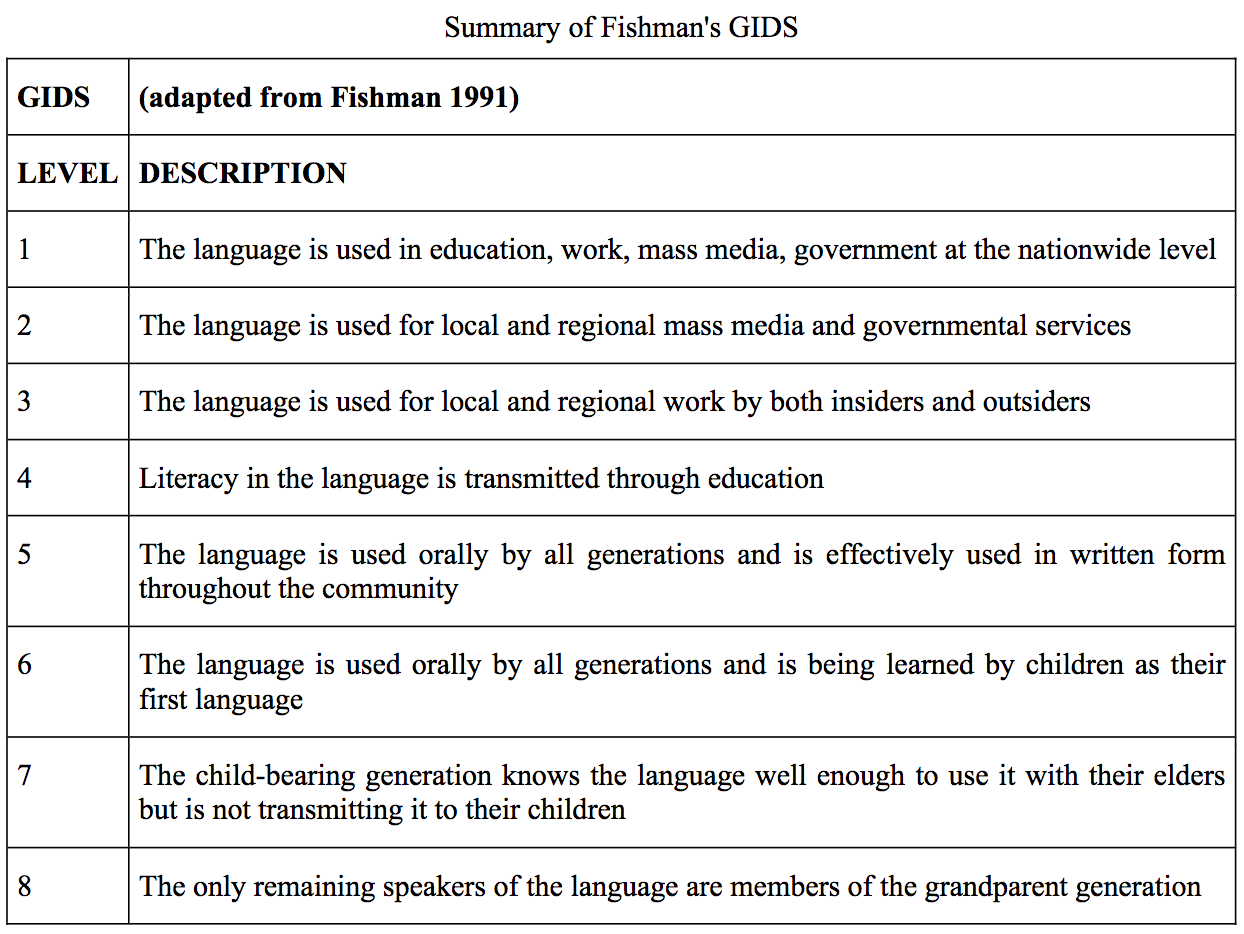
\includegraphics[width=.8\textwidth]{img/gids.png}
 \caption{A summary of GIDS from \citep[105]{lewis2010assessing}}
 \label{fig:gids}
\end{figure}

\subsubsection{The UNESCO measurement scale}
\label{subsec:unesco}

Chronologically, the UNESCO rating was the next major scale in the field. The United Nations Educational, Scientific and Cultural Organization (UNESCO) is a specialised agency of the United Nations. In 2001, at the 31st Session of the UNESCO General Conference, they officially recognised that biodiversity, cultural diversity, and linguistic diversity are related. This viewpoint is relatively recent, and reflects increasing appreciation that culturally diverse regions tend to collocate with biodiverse regions, and that saving diversity implies saving both \citep{nettle2000vanishing, maffi2001biocultural, anderson2006language, krauss2007keynote, gorenflo2012co} (as discussed explicitly in \citet{maffi2001}, of which all of the authors were also members of the UNESCO Ad Hoc Expert Group on Endangered Languages). Encouragingly, UNESCO clarified at this event that sustaining and encouraging linguistic diversity lies within their charter.

In their publication from that conference, \citet{brenzinger2003language} lay out nine different metrics for measuring language vitality: six evaluate the vitality, two language attitudes, and one related to urgency of documentation. The UNESCO system is rigorous in its refusal to apply a single score to a language, as that would smooth over the complexities of language usage. The six factors for vitality are: intergenerational language transmission (as with GIDS), absolute number of speakers, proportion of speakers within the total population, trends in existing language domains, response to new domains and media, and materials for language education and literacy.

For each of these, they further break rating down into categories. For instance, when regarding intergenerational language transmission, they specify six different possible ratings - safe, unsafe, definitively endangered, severely endangered, critically endangered, and extinct - and equate each rating with a score from 5 to 0. Here one of the primary issues with the UNESCO rating can be seen  (as pointed out by \citet{lewis2010assessing}) - namely, that 'safe' is an incredibly large category that needs more fine-grained categories, as it would account for any GIDS-rated language above Level 6.

The three other factors they consider are: governmental and institutional language attitudes and policies including official status and use; community members' attitudes toward their own language; and the amount and quality of documentation. Each of these is also rated on a null to five scale. For documentation, only a superlative rating of five would be considered to be more than low-resourced, as a four rating would be given to a language where "There are one good grammar and a number of adequate grammars, dictionaries, texts, literature, and occasionally updated everyday media; adequate annotated high-quality audio and video recordings." Although useful for linguists wishing to work in the language, this may not be enough for useful analysis and use by computational linguists. %TODO Should there be a section about linguists vs computational resources?

In Figure~\ref{fig:unesco}, an example rating using this system, from the appendix of \citet{brenzinger2003language} itself, is included to get some grasp of how these grades work in parallel.

Importantly, UNESCO clarifies that it does not suggest using one metric over another, and that adding up the numbers in the scales - however easy that might seem, as all of the measurements except speaking population are scalar and hold the same number of levels - would be insufficient and not ideal. "\textbf{Languages cannot be assessed simply by adding the numbers}; we therefore suggest such simple addition \textit{not be done} [sic]."

\begin{figure}
 \centering
 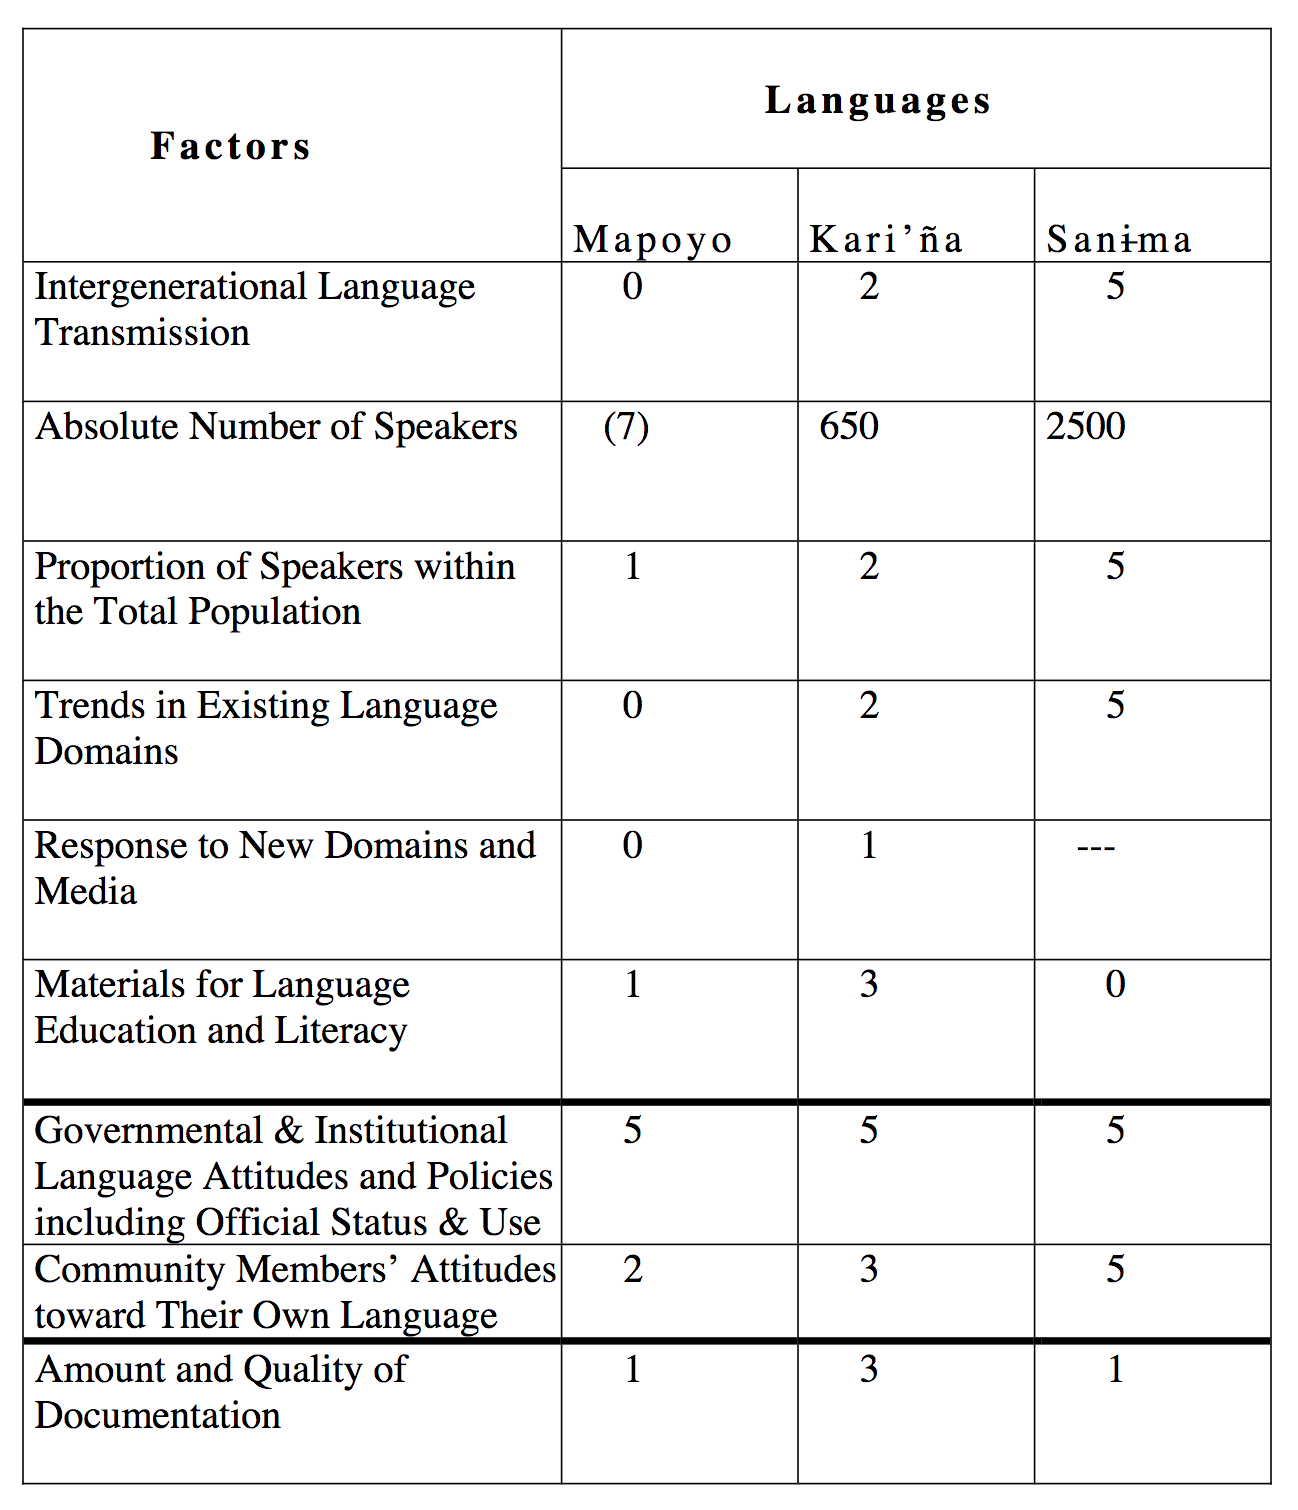
\includegraphics[width=.5\textwidth]{img/unesco.png}
 \caption{The UNESCO grading for three languages \citep[23]{brenzinger2003language}}
 \label{fig:unesco}
\end{figure}

The UNESCO ratings for languages are listed in the \textit{UNESCO Atlas of the World's Languages in Danger} \citep{unesco2014unesco}.

\subsubsection{The Extended GIDS (EGIDS)}

Lewis and Simons, the authors of Ethnologue \citep{lewis2009ethnologue}\footnote{Also a website available at \href{https://www.ethnologue.com/}{https://www.ethnologue.com/}. \last{May~2}}, pointed out some of the issues with GIDS which necessitate the creation of a new standard, and which could also eclipse or inform the UNESCO rating \citep{lewis2010assessing}. First, the levels are static, and don't account for directionality on the part of a language community up or down the strata. Second, there are language types which aren't included - for instance, there isn't a supranational level for extremely well-off languages, nor is there are level for extinct or dormant languages. Thirdly, GIDS focuses on intergenerational disruption in Level 5 and down, but in Level 4 and higher it focuses more on institutions, and this isn't accounted for well enough in the framework, which primarily focuses on parents as being the primary agents of language transmissions. Finally, the lower levels are not granular enough to cover the many complexities needed for language revitalisation groups.

EGIDS - the Expanded GIDS - serves these needs by providing more granular definitions. It also draws on the extensive knowledge of languages and their usage provided not only by Ethnologue, but also by the UNESCO Atlas and the community of linguists working with the Summer Institute of Linguistics (SIL), who fund and published Ethnologue. Figure~\ref{table:egids} shows the main categories, taken from the Ethnologue website.\footnote{\href{https://www.ethnologue.com/about/language-status}{https://www.ethnologue.com/about/language-status}. \last{May~2}} The table has been updated since \citet{lewis2010assessing}, in particular to also account for signed languages \citep{bickford2015rating}. The addition of a Level 0 and two levels beneath the scale are evident, as well as more granularity in the GIDS scale, such as can be seen with Level 6, which now has two levels, Level 6a Vigorous and Level 6b Threatened.

\begin{table}
\begin{center}
\begin{tabular}{|p{1cm}|p{3cm}|p{10cm}|} \hline
\textbf{Level}	& \textbf{Label}	& \textbf{Description} \\ \hline
0 	& International &  	The language is widely used between nations in trade, knowledge exchange, and international policy. \\ \hline
1 	& National &  	The language is used in education, work, mass media, and government at the national level. \\ \hline
2 	& Provincial &  	The language is used in education, work, mass media, and government within major administrative subdivisions of a nation. \\ \hline
3 	& Wider &  Communication 	The language is used in work and mass media without official status to transcend language differences across a region. \\ \hline
4 	& Educational &  	The language is in vigorous use, with standardization and literature being sustained through a widespread system of institutionally supported education. \\ \hline
5 	& Developing &  	The language is in vigorous use, with literature in a standardized form being used by some though this is not yet widespread or sustainable. \\ \hline
6a 	& Vigorous &  	The language is used for face-to-face communication by all generations and the situation is sustainable. \\ \hline
6b 	& Threatened &  	The language is used for face-to-face communication within all generations, but it is losing users. \\ \hline
7 	& Shifting &  	The child-bearing generation can use the language among themselves, but it is not being transmitted to children. \\ \hline
8a 	& Moribund &  	The only remaining active users of the language are members of the grandparent generation and older. \\ \hline
8b 	& Nearly &  Extinct 	The only remaining users of the language are members of the grandparent generation or older who have little opportunity to use the language. \\ \hline
9 	& Dormant &  	The language serves as a reminder of heritage identity for an ethnic community, but no one has more than symbolic proficiency. \\ \hline
10 	& Extinct &  	The language is no longer used and no one retains a sense of ethnic identity associated with the language. \\ \hline
\end{tabular}
\end{center}
\caption{Expanded Graded Intergenerational Disruption Scale \citep{ethnologuewebsite}}
\label{table:egids}
\end{table}

\citet{lewis2010assessing} also add another set of EGID levels which can be used to rate a language which is ascending in domains due to revitalisation efforts, which Figure~\ref{fig:egids-up} shows. This is generally useful, although it does suggest that a language uniformly descends or ascends, which may not be the case. The authors also spend time describing how to identify a language and decide which level best describes it.

\begin{figure}
 \centering
 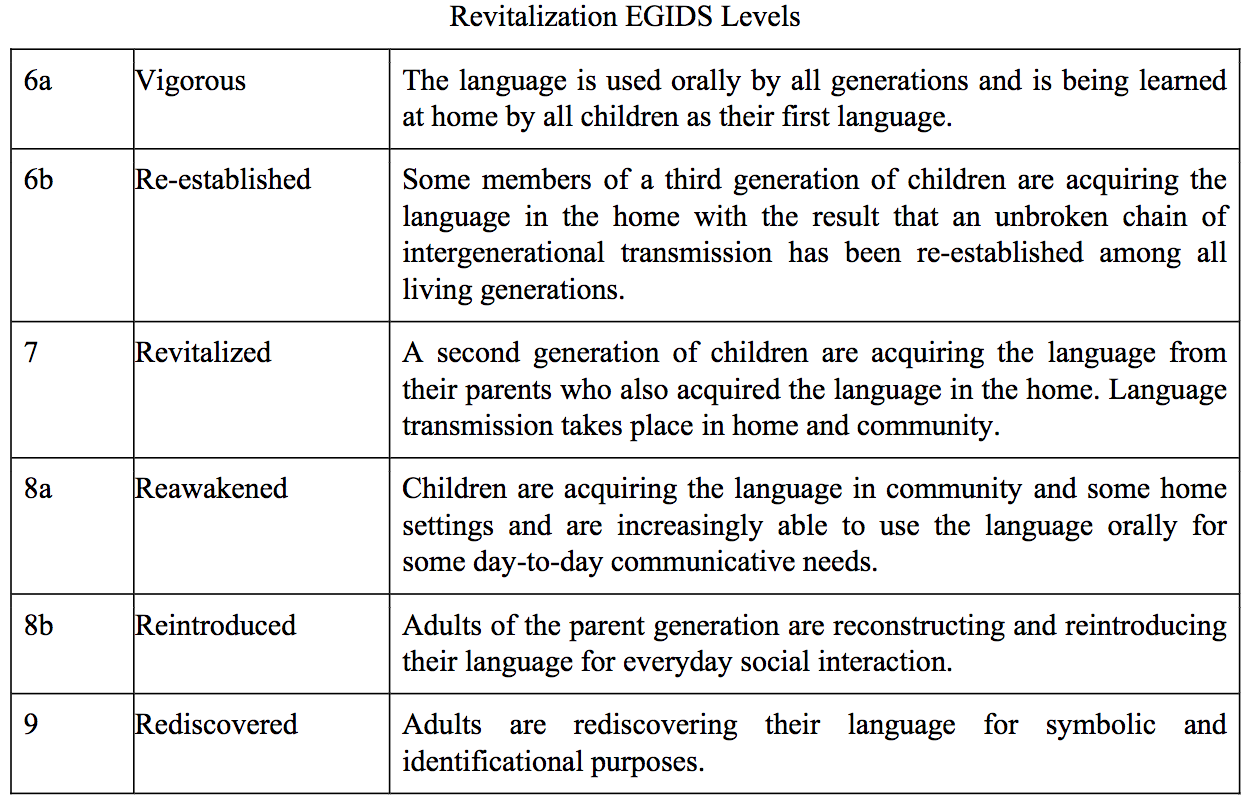
\includegraphics[width=.8\textwidth]{img/egids-up.png}
 \caption{A summary of EGIDS ascending levels \citep[117]{lewis2010assessing}}
 \label{fig:egids-up}
\end{figure}

They end with a quote from \citet{fishman2001can}, which explains further the purpose of EGIDS:

\begin{quote}
Thus, any theory and practice of assistance to threatened languages-whether the threat be a threat to their very lives, on the one hand, or a much less serious functional threat, on  the  other  hand-must  begin  with  a  model  of  the  functional  diversification  of languages. If analysts can appropriately identify the functions that are endangered as a result of the impact of stronger languages and cultures on weaker ones, then it may become easier to recommend which therapeutic steps must be undertaken in order to counteract any injurious impact that occurs. The purpose of our analyses must be to understand, limit and rectify the societal loss of functionality in the weaker language when  two  languages  interact  and  compete  for  the  same  functions within  the  same
ethnocultural  community  and  to  differentiate  between  life-threatening  and  non-life-threatening losses.
\end{quote}

\subsubsection{The Language Endangerment Index (LEI)}

Just as EGIDS expanded on GIDS, the Language Endangerment Index (LEI) was formed to resolve some of the issues with EGIDS, as well as to respond to GIDS, the UNESCO rating, and the rating in \citet{krauss2007classification}, another metric which focused almost exclusively on different ages of speakers and classified all languages with children speakers as 'stable', and all with over a million speakers as 'safe'. \citet{lee2016assessing} describe LEI for its use in The Catalogue of Endangered Languages (ELCat), part of the Google-powered Endangered Languages Project.\footnote{\href{http://endangeredlanguages.com}{http://endangeredlanguages.com}. \last{May~2}} The project isn't only sponsored by Google, but also by an American governmental National Science Foundation (NSF) grant\footnote{\href{https://www.nsf.gov/awardsearch/showAward?AWD\_ID=1058096}{https://www.nsf.gov/awardsearch/showAward?AWD\_ID=1058096}. \last{May~2}}, and is an ambitious project (like UNESCO and Ethnologue) to catalogue all languages and to provide specific metrics of language vitality.

The authors, in describing LEI, go into detail explaining how previous classifications, while they "highlight[s] the immensity of the problem at hand", can not easily apply to certain languages, and that these exceptions are critical to understanding whether the metrics are useful as opposed to being exceptions which prove the rule. Unlike the other papers, they explicitly mention some languages. For instance, they mention how \citet{dwyer2012tools} points out that Wutun, a Chinese-Tibetan-Mongolic language, is endangered due to a variety of factors, even if transgenerational transmission is not at risk - thus, GIDS or EGIDS may not satisfactorily categorise the language. A similar case could be made for Naskapi (see Section~\ref{sec:naskapi} for more on this).

The LEI uses four factors: intergenerational transmission, absolute number of speakers, speaker number trends (whether increasing or decreasing), and domains of use. Each of these is rated, like the UNESCO rating on a scale from null to five - however, unlike UNESCO, they add these numbers up to produce a single rating. The higher it is, the more likely the language is endangered. The scales are also somewhat different; for instance, number of speakers runs on orders of magnitude, with 100,000 being the top bound for a safe language (and not a million, like in \citet{krauss2007classification}).

\subsubsection{A response to qualitative metrics}
\label{subsubsec:response}

\citet{lee2016assessing} point out further issues with some of the other assessments - most notably that "while the UNESCO framework is broad and its factors comprehensive, it does not give an overall vitality score to the language being assessed, making it difficult to compare accurately across different language" and that "while an assessment of the type and quality of documentation is doubtlessly important because it helps indicate the potential for revitalization and the urgency of further research, it is not clear that the type and quality of documentation directly affects the vitality of a language." These two points are interesting, because they reflect how the situation of \citet{lee2016assessing} influences their judgement and their decision in making LEI at all. The authors were aware that they were being overtly quantitative in their approach:

\begin{quote}
Some may prefer a more nuanced examination of a language's vitality, with the view that the factors responsible for a language's endangerment are too complex to be compared across languages. Researchers of this view would rally against quantitative measures, stating that quantitative measures can hardly be accurate. ... ELCat researchers, while sympathetic to these points of view, maintain that without understanding and investigating fundamental common factors responsible for language endangerment, very little progress will be made in assessing language vitality and, consequently, less can be done to help communities preserve their languages. ELCat strikes a balance between these different perspectives.
\end{quote}

As \citet{grenoble2016response} points out, this misses the point of qualitative rebuttals, by claiming that accuracy is the most salient argument. It doesn't have to be, as there are more pressing concerns. For instance, all of the metrics were built on the assumptions that quantifying language endangerment is useful, and that assessment directly leads to empowering communities to revitalise their language. Neither of these are directly backed up by empirical research \citep{grenoble2016response}. More pressingly, language itself is not indisputably something that is countable or measurable, and to think so is to reflect Western, modernist ideologies surrounding language, viewing a language as a distinct entity which is formalised in writing and education. Language could be viewed alternatively as inextricable from the speaker and the utterance, and this view is more likely to be taken by language groups which view themselves as separate from a nation-state or an ethnographic group \citep{bodo2017language}. To view language otherwise is to confine language to a countable, commodifiable entity in a post-colonial sense, which affects how the language is viewed and can have real effects on language communities. Even viewing linguistic biodiversity as something to be 'saved' raises ideological  concerns, as Haspelmath (one of the main editors of \citet{wals}) notes.\footnote{\href{https://dlc.hypotheses.org/195}{https://dlc.hypotheses.org/195}. \last{May~2}} Indeed, post-colonial attitudes towards language endangerment may be endemic; \citet{newman1998we} certainly suggests that non-Western linguists cannot adequately document or revitalise their own languages without Western training, which presupposes that to be an informed researcher one must also conform to Western ideologies. Against this backdrop, \citet{lee2016assessing}'s claims that accuracy is something that can be attained seems to miss the mark; rather, the canonical approach to metrics is in itself a flawed approach that carries with it certain uncomfortable presumptions.

This thesis cannot hope to resolve these issues, nor is it meant to be an overview of the field of language vitality or endangerment as ideology. However, it is worth noting that metrics of language vitality do not exist in a vacuum, and that documentation and computational efforts are also a part of wider questions. Literacy is not a domain into which a language has to ascend to be seen as 'safe' or 'vital', and technological progress should not be viewed independently of an assessment of what exactly progress is.

Some things can be done, however. Terminologically, 'low-resource' is intentionally somewhat neutral, as compared to 'minority', 'endangered', or other terms that reflect Western viewpoints. Similarly, using the term {\it language vitality} as opposed to {\it language endangerment} "represents a significant shift in the representation of attitudes toward the rhetoric of indigenous languages to one away from dire predictions about endangerment to action-oriented attitudes about vitality and sustainability \citep{grenoble2016response}." These terms will be used for the rest of this paper, and any statements about resource development should be viewed as part of a narrower question of digital development (in the sense of building resources) for a specific, almost na\"ively countable view of language, unless otherwise specified (as in Section~\ref{sec:case-studies}).

% TODO Alexis: would be interesting to also discuss how these metrics might apply for the set of languages you're interested in (as defined in 2.1)

% Alexis: yes, in fact I think it's rather a different enterprise than defining language endangerment -- you may want to explicitly address the interaction between the two. what is your stance on the question? does lack of digital presence necessarily equate to language endangerment? (I think it's a very interesting question)


\subsection{Digital presence}

% I'll describe his assessment here, and explain why an alternative assessment would also be good. For instance, Wikipedia is, in my opinion, not a good judge of a language's health, as it is a closed ecosystem with diminishing returns for users who are bilingual.

Digital presence, briefly alluded to previously, can be thought of as the amount of language data available through digital sources. A looser definition could be 'the amount of written text on the web', but this would miss out on several important considerations. First, linguistic data does not have to be written to be digitally encoded; videos and audio data are both examples of digital content which is often digitally encoded. In some cases, pictures are also relevant, especially for signed languages or for examples of written text, such as in the millions of scans of papyrus from the Egyptian city of Oxyrhynchus, which are being translated using a crowd-sourced system by thousands of volunteers \citep{williams2014computational}, or for other language mediums, such as the khipu knot system used by the pre-Columbian Incan civilisation \citep{quilter2002narrative}. Secondly, the web (hereafter meant to refer to the World Wide Web) is not the only corpus of knowledge, nor is it the only network through which data can be accessed. Trivial example of other corpuses would be local files collected by individual field researchers that are backed up on hard drives; a similar example of another network would be a local area network in offline areas, or a university intranet.

However, the digital sphere can best be thought of schematically as a new domain for language use, and it is overwhelmingly today represented on the web. Ten years ago, it was fashionable to include references to the web "as a a corpus" (as \citet{scannell2007crubadan}, for instance, cited \citet{resnik1999mining, ghani2001mining, kilgarriff2001web}, although the latter two were in reference to low-resource languages); today, it is more common to cite studies on digital natives such as the 20,000 citation-strong \citet{prensky2001digital} paper,\footnote{This number is from Google Scholar (\href{https://scholar.google.com}{https://scholar.google.com}) accessed April 9, 2018.} or to assume that the web, and occasionally phone networks, are the main locations for digital communication. The web is ubiquitous; not only are more than half of the global population connected to the internet,\footnote{\href{https://www.internetworldstats.com/stats.htm}{https://www.internetworldstats.com/stats.htm}. \last{May~2}} but the internet, in developed countries, is used for all levels of communication, such as education, work, mass media, and in the home and local communities. Digital presence, then, is functionally the amount of usage on the web.

\subsubsection{Finding resources}
\label{subsec:finding-resources}

There are several resources which can be used to judge the amount of corpora for a language on the web, outside of papers defining metrics to judge these languages and to state whether they are endangered or thriving. The main resource for low resource languages is almost certainly the Cr\'ubad\'an project, developed by \citet{scannell2007crubadan}.\footnote{\href{http://crubadan.org/}{http://crubadan.org/}. \last{May~2}} This is a massive crawler which looks for documents with trigram frequencies for particular languages by checking against a seed corpus for under-resourced languages developed from Wikipedia, the Jehovah's Witness translations, and translations of the UN Declaration of Human Rights (UNHR). It is often the only corpus for a low resource language on the web, as is the case with Naskapi (see Section~\ref{sec:naskapi}).

Often, a translated Bible is the next best place to look for digital content. Biblical translations are so common as a first resource that there is a body of research that uses partial or full translations of the Bible for training NLP systems as a result \citep{chew2006evaluation, agic2015if}. However, finding the bible or UNHR is often difficult. In these cases, it is best to look for aggregators of data. There are large projects which hold resources for linguists - for more, see Section~\ref{subsec:resource-aggregators}. However, these resources aren't always directly reflective of a language's digital presence, but rather of the scope of resources available to computational linguists and natural language processing experts. They satisfy a different need, and tools such as Perseus\footnote{\href{http://www.perseus.tufts.edu/hopper/}{http://www.perseus.tufts.edu/hopper/}. \last{May~2}} might show that there is work done on Latin, but it doesn't mean that there is a large Latin-speaking community that could be measured. Instead, organic corpora - such as collected from the web by Cr\'ubad\'an - are most likely the best ways of measuring a language's foothold on the web.

\subsubsection{Metrics for digital presence}

\citet{kornai2013digital} outlined the first major metric for describing digital presence for a language. These metrics are needed because normal metrics aren't directly transferable to digital presence, as digital linguistic data is decoupled from speakers (it can survive beyond them), and because the digital domain is only one of a variety of domains for language usage. He divided languages into four possible categories: {\it Thriving}, {\it Vital}, {\it Heritage}, and {\it Still}. These can be thought of as a gradient, with digital ascent being the process of a language moving up the scale. Only 16 languages would be considered Thriving, all of which would be rated at 1 or higher on the EGIDs scale. Vital languages are those which may be in danger in the next hundred years, or show few signs of digital ascent - but they have a large population of speakers and at least some resources, such as a Bible or the UNHR; Heritage languages are dead or historic languages such as Latin which have large online presences that do not relate directly to a living language community; and Still languages show little to no presence on the web at all (although note that this does not mean that they endangered or moribund outside of the web.)

Kornai looks at five confluent factors; demographics, prestige, the identity function of the language, the level of software support, and Wikipedia presence for a language. Demographics and community size can be gathered by doing a quantitative analysis of all public data available in a language on the web, and by using this data size as a proxy for the amount of speakers of a language using the digital space. This has obvious limits, which Kornai points out, in that the data may not accurately reflect the amount of users, in that it is limited to public data accessible by researchers, and in that it doesn't give an accurate representation of passive consumption of multilingual data. It would be worth adding that this also doesn't give an accurate count of multilingual usage of a language. Prestige is an obvious factor for digital ascent; when a language community views one language more highly than another, it is more likely to create digital content in one than the other, regardless of social policies and to some extent speaker populations. Identity function relates largely to certain historical languages, like Latin and Classical Chinese, which have large corpora online but should not be considered in the same grouping as more vibrant, living languages.

Software support as a factor in digital presence could be identified with a variety of different metrics. Kornai lists various stages for a language on the road of digital ascent. First, localisation of internalisation (often expressed using the shorthand l10n or i18n, where the numbers refer to the length of the words) of the language script is the major milestone that separates languages which are ascending from still languages. While many scripts use the more common Roman, CJK, Cyrllic, or Arabic alphabets, there are hundreds which do not, and these languages have specific Unicode considerations which need to be met for the language to be used adequately. The next step would be word-level tools, such as dictionaries, stemmers, and spellcheckers - all of which depend, at some point, on standardisation (but not s13n) of the language. Finally, sentence level tools such as automatic translators can be used. Regarding support, the question of a language's status is straightforward: is there language support for an operating system provided by Apple or Microsoft? If so, then it is likely that the language is thriving or vital. If not, there is almost zero chance of it being so. Kornai also used the Cr\'ubad\'an Project, UHDR and biblical presence, and presence on Omniglot and OLAC.

Kornai found that Wikipedia was a good example of a first port-of-call for language speakers on the web, and that it could be used to show that a language was "crossing the digital divide."

\begin{quote}
The reason is that children, as soon as they start using computers for anything beyond gaming, become aware of Wikipedia, which offers a highly supportive environment of like-minded users, and lets everyone pursue a goal, summarizing human knowledge, that many find not just attractive, but in fact instrumental for establishing their language and culture in the digital realm. To summarize a key result of this study in advance: \emph{No wikipedia, no ascent} [sic]. \citep{kornai2013digital}
\end{quote}

Ultimately, Kornai found that the best indicator of a language's digital presence was their EGIDS rating. "The next best set of features indicated the quality of the wikipedia, followed by the number of L1 speakers, the size of the Cr\'ubad\'an crawl, the existence of FLOSS spellcheckers, and the number of online texts listed in OLAC." \citep[6]{kornai2013digital} Overall, only 5\% of the world's languages were seen as digitally ascending; like most results from this field, an increasingly dire statistic. As \citet[10]{kornai2013digital} writes:

\begin{quote}
Unfortunately, at a practical level heritage projects (including wikipedia incubators) are haphazard, with no systematic programmes of documentation. Resources are often squandered, both in the EU and outside, on feel-good revitalization efforts that make no sense in light of the pre\"{e}xisting functional loss and economic incentives that work against language diversity \citep{ginsburgh2011many}.
\end{quote}

However, others have noted that Kornai may have been early in his predictions that most languages will not digitally ascend \citep{gibson2016assessing}.

In a follow-up paper, \citep{kornai2015new} proposed adding a single number scale to assess digital ascent: "For the assessment we propose a simple log-linear formula that derives a single number {\emph D} (digital vitality index) as a weighted sum of well-understood components such as the EGIDS ranking, (log) number of L1 speakers, (log) size of wikipedia, adjusted for quality, (log) crawl size, the existence of FLOSS spellcheckers, etc." The EGIDS ranking was considered objective, given that SIL linguists are generally interested in longer term work with communities as opposed to relatively short-lived or quantitative studies done by computational linguists. This log-linear formula was innovative for cleaning wikipedia, in particular, as it removes the likelihood of large wikipedias built by hobbyists with bots as being indicative of large language communities.

\citet{gibson2016assessing} extends Kornai by adding two separate statuses for languages - that of {\it Emergent} and {\it Latent}. Emergent languages are those where there is data, but it is privately hidden in messaging applications or cellphone usage, and unlikely to be accessible by the crawlers and corpora agglomeration tools used in \citet{kornai2013digital}. These would be identified by researchers in the field, and do not need to have locale or i18n setups before inception. Gibson cites Arabizi (as noted by \citet{darwish2013arabizi}), where numbers are used for sounds not present in standard Arabic, as an example; another might be the use of a forward slash to denote accents in early Irish Gaelic forums, as noted by \citet{scannell2007crubadan}. Latent languages are languages which meet the following criteria: "stable intergenerational transmission of the language, an available model of writing the language, the availability of appropriate technology and infrastructure (internet, mobile phone coverage), fonts in which to write the language in the desired script, and communal desire to see the language used digitally." If all of these are met, then the language could ascend beyond still into vital. Such languages would be admittedly impossible to find by measurements, but this category would be helpful for linguists working in the field to determine how to best work with the language community to help bootstrap language development. Gibson also redefined {\it Still}, which \citet{kornai2013digital} had marked as languages which are 'unable' to ascend, while here they are merely 'unlikely'.

A more recent metric was also introduced in a draft by \citet{soria2017digital}, for the purposes of helping digital language planning for the EU, as part of the Digital Language Diversity Project.\footnote{\href{http://www.dldp.eu/content/reports-digital-language-diversity-europe}{http://www.dldp.eu/content/reports-digital-language-diversity-europe}. \last{May~2}} Their scale has the following states: {\it Pre-digital}, {\it Dormant}, {\it Emergent}, {\it Developing}, {\it Vital}, and {\it Thriving}. Like Gibson, they exclude Kornai's {\it Heritage} status (oddly noting that Gibson also included it, which he hadn't for the same grounds), without sufficient explanation as to why dead languages are not relevant when there are communities based around them, some of which are communities with thousands of L2 speakers. %(NOTE: Write a paper about this. %TODO: Remove this comment after review from Alexis).
Dormant would be equitable to Latent, while Pre-digital would apply to languages without internet or cell connectivity for the speaking population. Emergent through Thriving are largely matters of scale. While Kornai used proxies for the five factors he mentioned, Soria et al. note that such factors are difficult to quantify; they remedy this by focusing on three indicators: "a group pertaining to a language digital {\it capacity} [sic], a group related to a language digital {\it presence and use}, and a group related to a language digital {\it performance}." \citep[5]{soria2017digital} An example of how these are used can be seen in Figure~\ref{fig:dldp}.

\begin{figure}
 \centering
 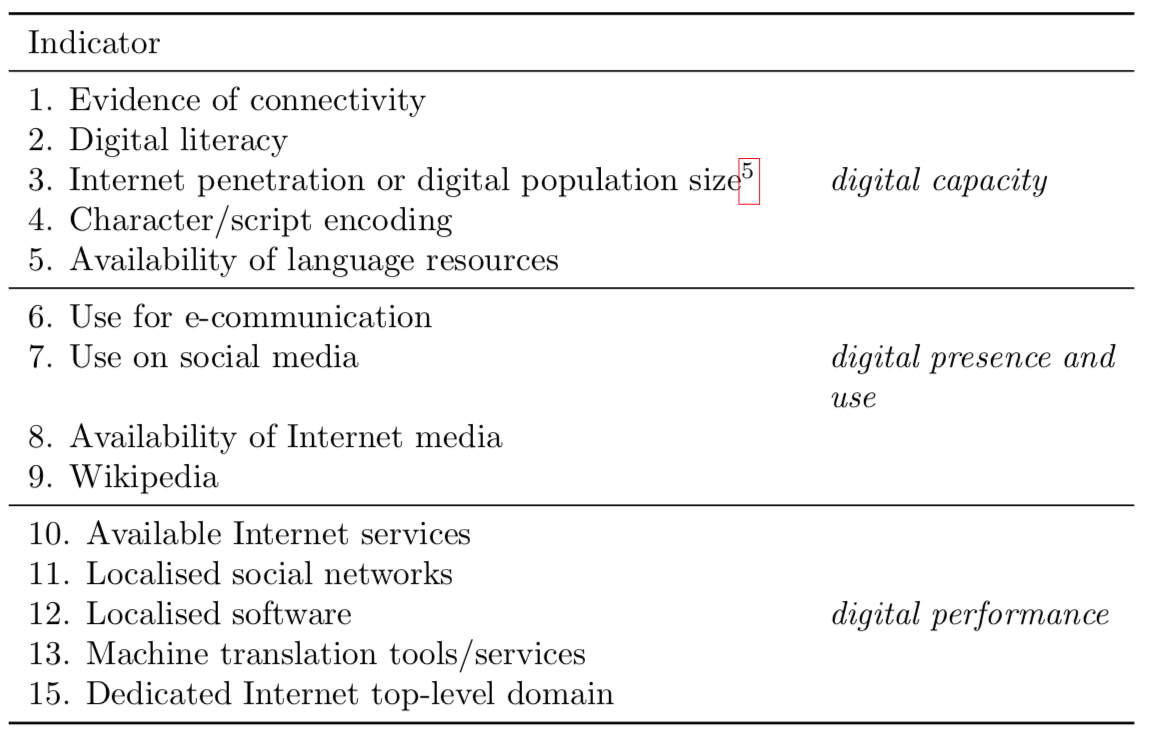
\includegraphics[width=.8\textwidth]{img/dldp.png}
 \caption{Indicators of digital vitality \citep[6]{soria2017digital}}
 \label{fig:dldp}
\end{figure}

\citet{soria2017digital} go into depth about each of these factors. As an example, for localised software, they propose the following scale in Table~\ref{table:dldp-software}. They explain, for each scale, how to find information - for instance, they suggest asking local researchers and community members about the usage of "Windows, Mac OS X, Linux, Android, iOS, Microsoft Office, LibreOffice, Firefox, Chrome, Internet Explorer, Thunderbird, Adobe Creative Suite, Gimp" for judging localised software. However, they do not show metrics on any languages judged according to this scale, and they don't make it clear whether or not the different metrics ought to be summed to come up with a single number (an issue which \citet{lee2016assessing} raised with the UNESCO rating). In conclusion, while this is an interesting and in-depth metric, its wider applicability is not clear.

\begin{table}
\begin{center}
\begin{tabular}{|p{2cm}|p{1cm}|p{10cm}|} \hline
Label & Grade & Localised software \\ \hline
none & 2 & Neither operating system nor general purpose soft- ware localised in the language\\
limited & 3 & At least one operating system (either desktop or mo- bile, either open or commercial) localised in the language \\
medium & 4 & At least one desktop and one mobile operating system (either open or commercial) + some general purpose software (a word processor and a browser) localised in the language\\
strong & 5 & Most used operating systems and general purpose software localised in the language; some specific purpose application software localised.\\
advanced & 6 & Main operating systems and application software localised in the language.  \\ \hline
\end{tabular}
\end{center}
\caption{Scale for Localised Software \citep[21]{soria2017digital}}
\label{table:dldp-software}
\end{table}

Each of these metrics suffers from growing pains. For instance, there is no metric as of yet which ranks English in its own category - something which was seen as a large enough issue to cause the EGIDS authors to add another null ranking for supranational languages. %(TODO: Write a paper on this)
As well, there hasn't been an integrated approach looking at quantitative and qualitative measurements together. The most substantial work on this has been Kornai's team, which has worked with funding from SIL International on a Digital Language Vitality database.\footnote{\href{https://hlt.bme.hu/en/projects/lingvit}{https://hlt.bme.hu/en/projects/lingvit}. \last{May~2}} However, the future for this work as, at this moment, unclear (Kornai in personal communications, 2018).

% There's no higher scale - what separates English from French?
% What about coding _in_ a language? How many languages have native computer languages?



% The State of endangered languages and computational linguistics
%\subsection{Defining Endangered Languages}
%\subsection{What are computational resources}
% !TEX root = thesis.tex
\section{Resources}
\label{sec:resources}

It makes sense at this point (if not earlier), to discuss what language resources are. There are two main types of resources: corpora and tools which act on corpora. They are inextricably linked, but the approaches towards building, archiving, and using either differ. This section seeks to answer one question: what resources are needed to take a language from no resources, to a thriving language with a large digital presence?

For digital vitalisation, \citet{kornai2015new} proposes working on a pyramid approach: first build a corpus with active and engaged speakers, then l10n and i18n support; then word-level tooling such as spell checkers and morphological analysers; phrase and sentence level tooling such as parsers; and finally speech and character recognition and machine translation. This, in general, follows how most language development progresses. However, a finder grained understanding of the tools would be illuminating. While an exposition of all possible natural language processing tools is beyond the scope of this thesis, it is worth going into some depth about some of them.

It is worth noting here that there are different groups which work on each of the stages of language development. Abstractly, these could be defined as language communities and linguists, and the fields of computational linguistics and natural language processing (NLP). The first group are those - often not computational linguists by training or NLP researchers - who want their own language or the language they are studying to exist digitally and in some form. The initial step is generally to adopt any language script, whether  pre\"{e}xisting or ready-made for the language by linguists (for examples of this, see the Endangered Alphabets Project\footnote{\href{http://endangeredalphabets.com/}{http://endangeredalphabets.com/}}) into Unicode, a standard for consistent character representation.\footnote{\href{https://unicode.org/}{https://unicode.org/}} There are linguistic research groups that focus on this problem; for instance, the Script Encoding Initiative at Berkeley.\footnote{\href{http://linguistics.berkeley.edu/sei/index.html}{http://linguistics.berkeley.edu/sei/index.html}}

Some of the people involved in this process may be computational linguists. \citet{bender2016linguistic} makes a distinction between the fields of computational linguistics and NLP: "computational linguistics is used to describe research interested in answering linguistic questions using computational methodology, while natural language processing describes research on automatic processing of human language for practical applications." It should be clear here that computational linguistics is a subfield of linguistics, and that the two are not always in sync, as for instance \citet{kay1997proper} points out when discussing improving machine translation (ML) by using informed linguists. \citet{bender2010grand, bender2016linguistic} goes further, suggesting that understanding language typology can drastically help with multilingual NLP. Many experts in NLP would not consider themselves computational linguists, but developers, just as many language developers would not consider themselves linguists. While navigating the field or looking at resources, it is important to keep these distinctions in mind, as they inform narratives concerning resource generation, scope, and efforts.

\subsection{Resource Aggregators}
\label{subsec:resource-aggregators}

I've already mentioned that Cr\'ubad\'an \citep{scannell2007crubadan} is a good location to find monolingual texts from the web; however, this is but one of an almost infinite amount of corpora that might be of use to linguists, language activists, and to NLP practitioners. To find other resources can be an overwhelming task. To help solve this issue, there are a non-trivial number of large organisations and databases where it is possible to find resources - dictionaries, academic references, and occasionally software - on low resource languages. \citet{unesco11directory} for instance itemises hundreds of such resources. To give more of an idea of what these resources are like, here are some major examples:

\begin{itemize}
\item The Unicode Common Local Data Repository (CLDR) "provides key building blocks for software to support the world's languages, with the largest and most extensive standard repository of locale data available."\footnote{\href{http://cldr.unicode.org/}{http://cldr.unicode.org/}} There are dozens of scripts available in Unicode.\footnote{\href{https://www.unicode.org/standard/supported.html}{https://www.unicode.org/standard/supported.html}}

\item The Endangered Languages Project (ELP), described above and in \citet{lee2016assessing} and online\footnote{\href{http://www.endangeredlanguages.com/}{http://www.endangeredlanguages.com/}} has information on many under resourced languages.

\item Ethnologue, which is both a book \citep{lewis2009ethnologue} and an online resource,\footnote{\href{https://www.ethnologue.com/}{https://www.ethnologue.com/}} is the most comprehensive resource describing the world's languages, such as population size and the general geographic locations of speakers. It is published by SIL International, an evangelical Christian non-profit organisation, and has proprietary paywalls for repeated access to content. Many SIL entries for specific languages include academic references.

\item Glottolog\footnote{\href{http://glottolog.org/}{http://glottolog.org/}} is an open source alternative to Ethnologue, developed at the Max Planck Institute for Evolutionary Anthropology. It has over 180,000 references, with information on over eight thousand languages. \citep{hammarstrom2015glottolog}

\item Omniglot, "the online encyclopaedia of writing systems and languages",\footnote{\href{http://omniglot.com}{http://omniglot.com}} contains around writing information for around a thousand languages. \citep{ager2008omniglot}

\item The Online Database of Interlinear Text (ODIN)\footnote{\href{http://odin.linguistlist.org}{http://odin.linguistlist.org}} is a multilingual repository of annotated language data for 1274 languages.\footnote{Noted as of January 13, 2010; Accessed April 17, 2018. \href{http://odin.linguistlist.org}{http://odin.linguistlist.org}} The database is formed by crawling scholarly articles on the web and looking for interlinear glossed text (IGT), an industry standard for displaying corpora in academic linguistics by displaying the original datum, a morphosyntactic gloss, and a translation. These data are not massive, but they are useful in particular for training algorithms on structured data. As well, "ODIN was developed as part of the greater effort within the GOLD Community of Practice \citep{farrar2007gold} and the Electronic Metastructure for Endangered Languages Data efforts (EMELD)\footnote{\href{http://emeld.org/}{http://emeld.org/} and \citet{farrar2002common}}, whose goals are to promote best practice standards and software, specifically those that facilitate interoperation over disparate sets of linguistic data." \citep{lewis2010developing}

\item The Open Language Archives Community (OLAC), a worldwide virtual library of language resources \citep{simons2003open}.\footnote{\href{http://www.language-archives.org/}{http://www.language-archives.org/}}

\item Wikipedia,\footnote{\href{https://www.wikipedia.org/}{https://www.wikipedia.org/}} "the largest and most popular general reference work on the Internet" \citep{wiki:Wikipedia} has a nontrivial amount of articles on low-resource languages, many of which have references themselves to Scholarly work. \citet{kornai2013digital}, among others, notes that Wikipedia is one of the first ports-of-call for new language communities, and while it is not a precondition for having corpora on the web, it is a {\it sine qua non} for digital vitalisation. Thus Wikipedia has two purposes; documenting the language and its community (for instance, in the Naskapi Language article\footnote{\href{https://en.wikipedia.org/wiki/Naskapi\_language}{https://en.wikipedia.org/wiki/Naskapi\_language}}), and providing a space for corpus development in the target language itself.

\item The World Atlas of Language Structures (WALS) is a directory typological features which also includes academic references for many of the over two thousand languages presented. WALS is a curated resource, largely made by a team of 55 experts, and hosted by the Max Planck Institute for Evolutionary Anthropology (the same as Glottlog, and as other resources such as PHOIBLE\footnote{\href{http://phoible.org/}{http://phoible.org/}} \citep{phoible} and DOBES\footnote{\href{http://dobes.mpi.nl/}{http://dobes.mpi.nl/}} \citep{wittenburg2003dobes} related to taking an inventory of language structures). \citep{wals}

% are the LREMap ([2], [17]), the CLARIN Virtual Lan- guage Observatory 16, the catalogues of Linguistic Data Consortium17, ELRA18 and META-SHARE19. From soria 2017

%  ELRA, LDC, NICT Universal Catalogue, ACL Data and Code Repository, OLAC, LT World.

\end{itemize}

There are other resources: the CLARIN Virtual Language Observatory\footnote{\href{https://vlo.clarin.eu}{https://vlo.clarin.eu}}, the Linguistic Data Consortium at UPenn,\footnote{\href{https://www.ldc.upenn.edu/}{https://www.ldc.upenn.edu/}} the ELRA,\footnote{\href{http://catalog.elra.info}{http://catalog.elra.info}} META-SHARE,\footnote{\href{http://www.meta-share.eu/}{http://www.meta-share.eu/}} the Association for Computational Linguistics' Wiki,\footnote{\href{https://aclweb.org/aclwiki}{https://aclweb.org/aclwiki}} the NICT Universal Catalogue,\footnote{\href{https://www.nict.go.jp/index.html}{https://www.nict.go.jp/index.html}} LT World\footnote{\href{http://www.lt-world.org/}{http://www.lt-world.org/}} and so on. Providing an exhausting list would be exhausting - more pertinently, now that it is clear that there are resources, what ones are relevant to low resource languages?

\subsection{BLARK and LRE maps}
\label{subsec:blark-and-lre-maps}

\citet{soria2017digital} briefly mention "digital language survival kits" as one of the motivations for their paper - these are explicated more fully on the Digital Language Diversity Project's site.\footnote{\href{http://www.dldp.eu/en/content/digital-language-survival-kit}{http://www.dldp.eu/en/content/digital-language-survival-kit}} This project is an EU initiative, through the Erasmus+ programme, and it aims to identify needs and provide "kits" for certain European low resource languages - specifically Basque, Breton, Karelian and Sardinian.

The use of the word "kit" is informative, as there is  pre\"{e}xisting literature on this topic in BLARK, or Basic Language Resource Kit. BLARK was developed by a joint initiative between the European Network of Excellence in Language and Speech (ELSNET), a European international umbrella for 145 different organisations in 29 countries, and the European Language Resources Association (ELRA), and first outlined in 1998 \citep{krauwer1998elsnet}. The BLARK is defined as the "minimal set of language reosources that is necessary to do any precompetitive research and education at all." \citep[4]{krauwer2003basic} In general, this comprises "written language corpora, spoken language corpora, mono- and bilingual dictionaries, terminology collections, grammars, modules (e.g. taggers, morphological analysers, parsers, speech recognisers, text-to-speech), annotation standards and tools, corpus exploration and exploitation tools, bilingual corpora, etc."

\citet{krauwer2003basic} has a comprehensive matrix in the appendix outlining technology that would be needed to provide a BLARK for Dutch, as outlined in a workshop documented in \citet{binnenpoorte2002towards}. In another paper, \citet{maegaard2006blark} under NEMLAR (Network  for  Euro-Mediterranean  LAnguage  Resources) outlined the specific needs that BLARK specified which could be applied to Arabic, and actions which researchers took in order to develop resources to best fill in the grid. Both of the BLARK grids for Arabic provided in that paper are included here, in Figures~\ref{fig:blark1} and \ref{fig:blark2}, as they very usefully show not only the state of human language technology (HLT) resources for Arabic at the time, but also the categories thought sufficient. These categories - "prosody prediction", "alignment", "shallow parsing", and so on - are all terms which refer to a suite of resources that each reflect hundreds of papers from within the computational linguistics community.

\begin{figure}
 \centering
 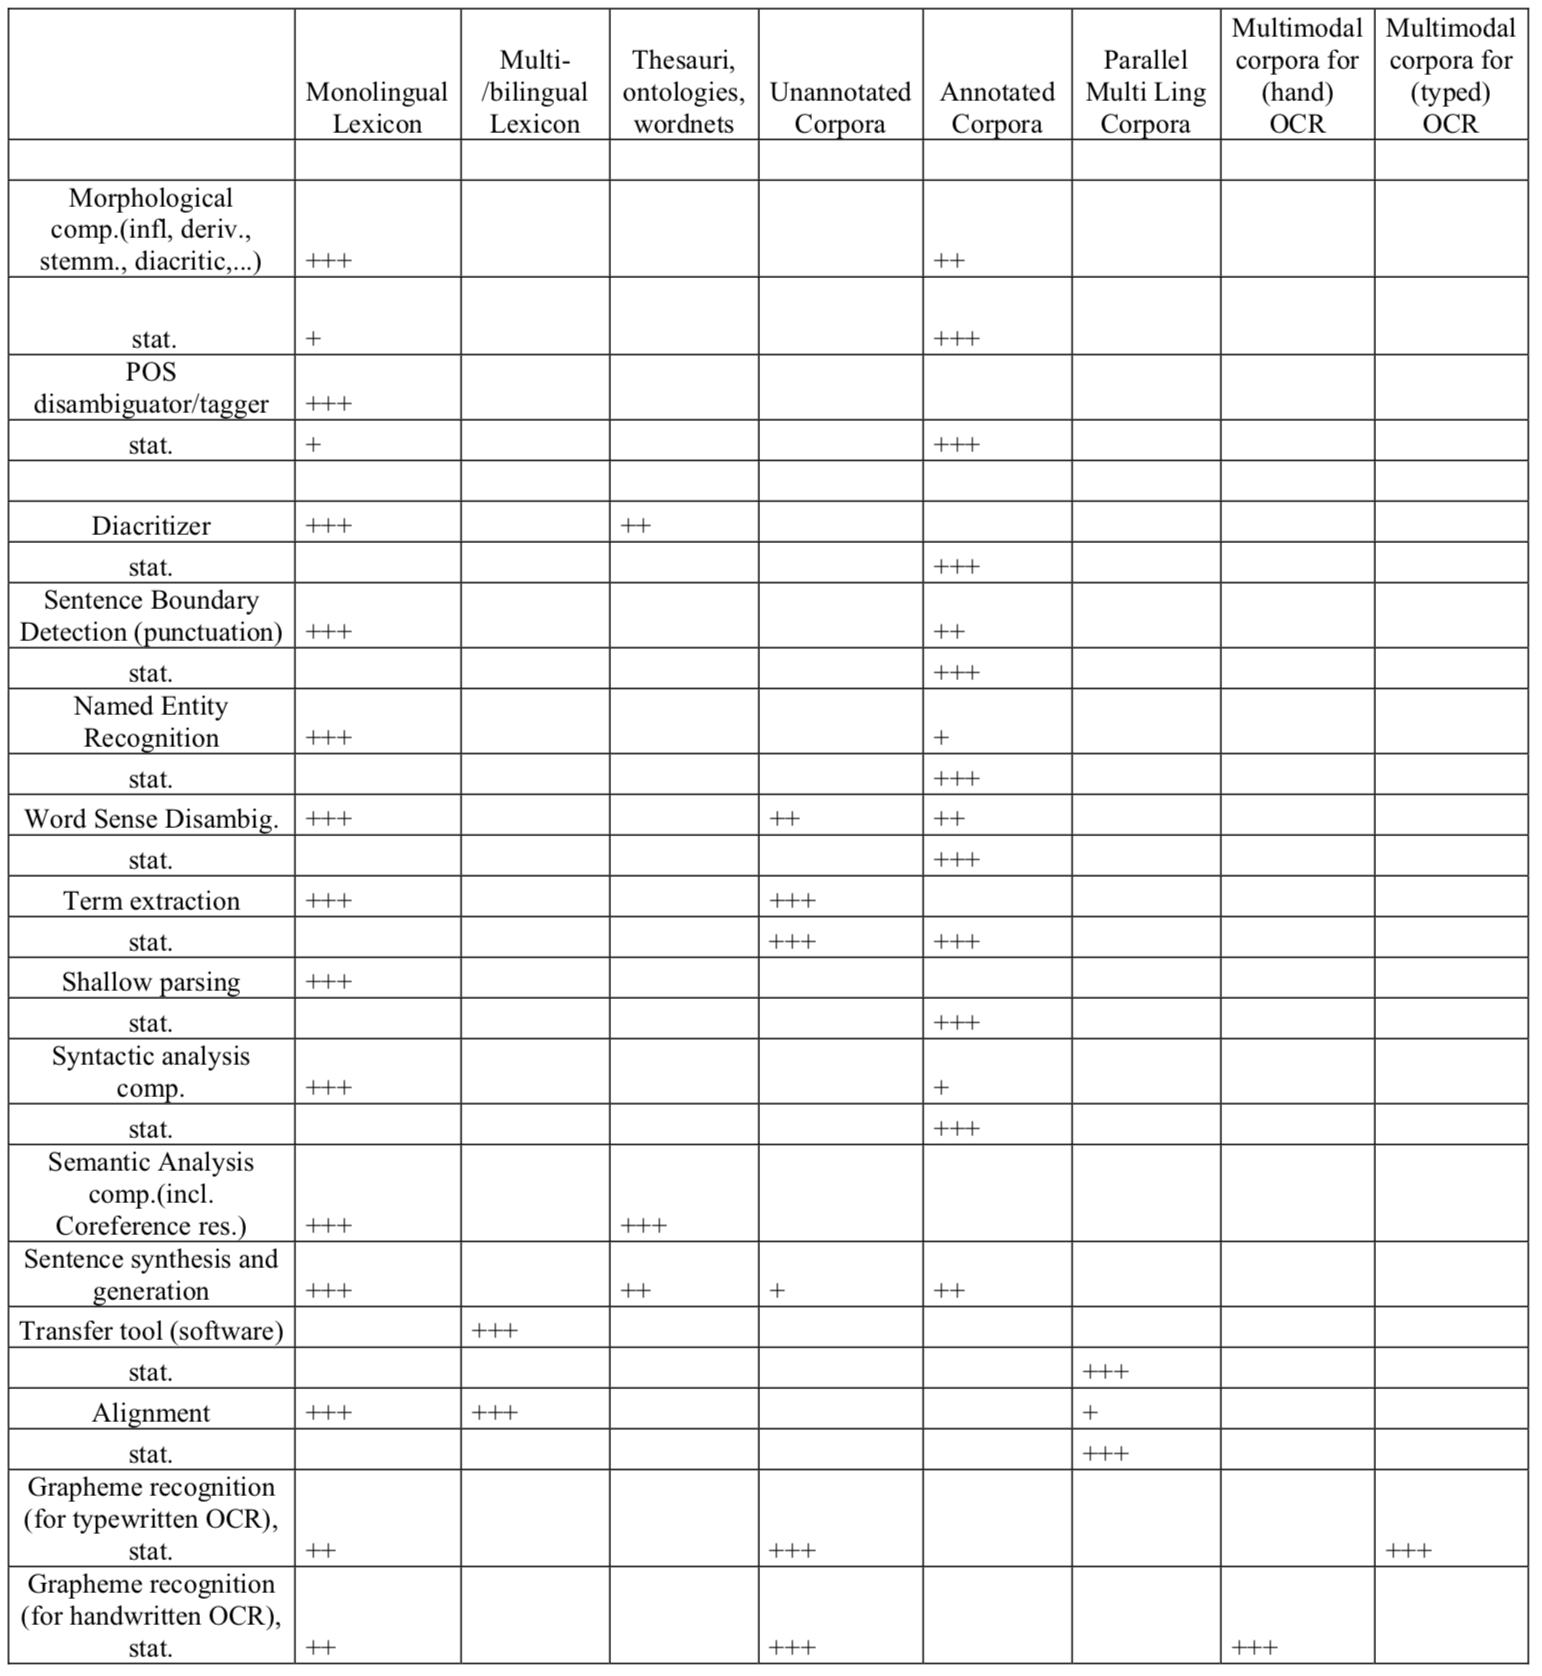
\includegraphics[width=1\textwidth]{img/blark1.png}
 \caption{A BLARK graph for Arabic, with written language applications and corresponding HLT modules, marked with importance \citep[775]{maegaard2006blark}}
 \label{fig:blark1}
\end{figure}

\begin{figure}
 \centering
 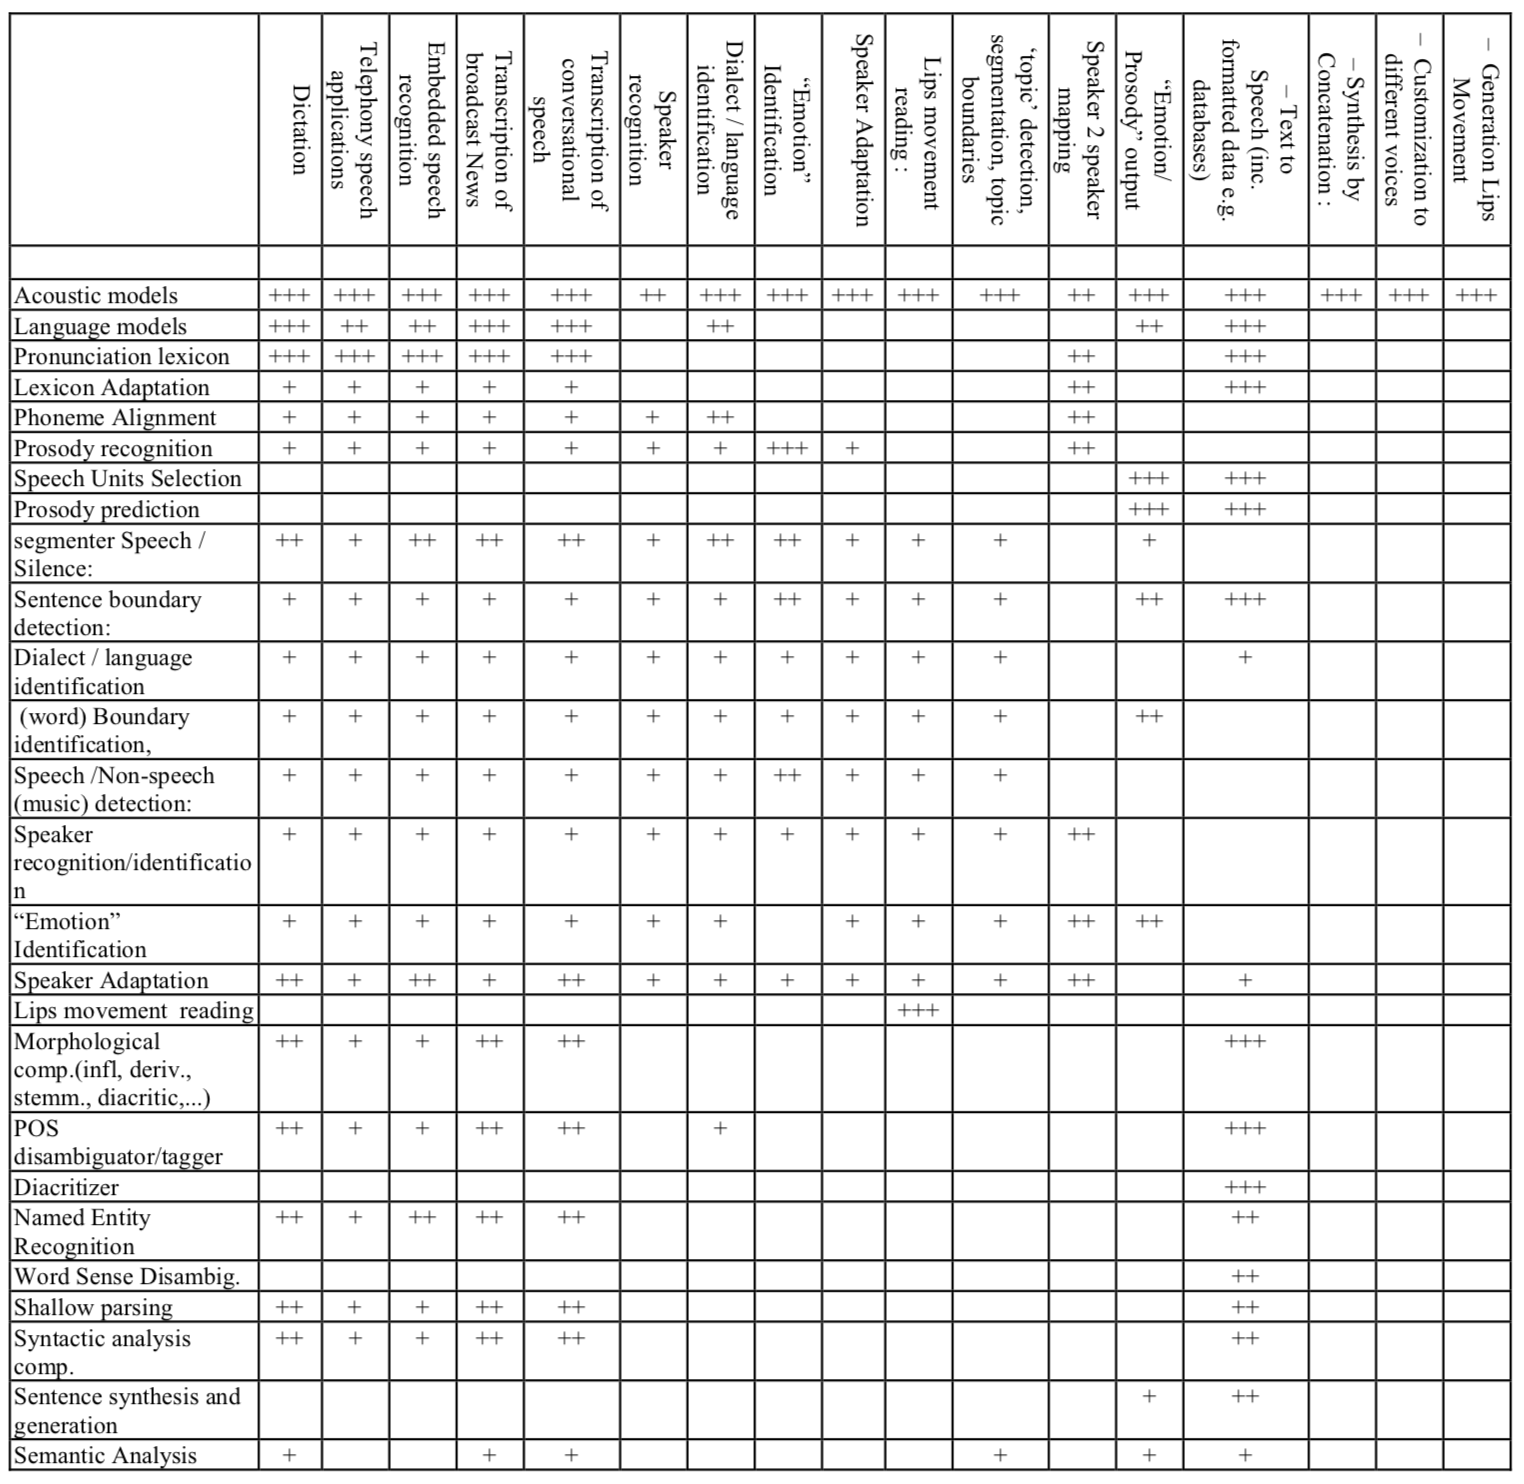
\includegraphics[width=1\textwidth]{img/blark2.png}
 \caption{A BLARK graph for Arabic, with speech language applications and corresponding HLT modules, marked with importance \citep[776]{maegaard2006blark}}
 \label{fig:blark2}
\end{figure}

The BLARK process - auditing a language, using a grid to identify what corpus and resource needs are necessary for language resources - has now been applied to Swedish \citep{elenius2008language} and Bulgarian \citep{simov2004language}, and numerous South African languages \citep{grover2011south}, among others.

Unfortunately, BLARK (or ELARK, purportedly a more sophisticated version of BLARK for industry described in \citet{mapelli2003report}, according to \citep{grover2011south}) is a large grid, and may not work for languages without extensive funding models or support. For this, there is a smaller BLARK version, the BLARKette, which should work for low resource languages (although how a smaller version of a minimal set could be provided usefully is not clear).

\begin{quote}
In order to accommodate this problem we have proposed the definition of a scaled down, entry-level version of the BLARK, targeting exclusively the research and (especially) the education community. It should be light and compact, not too demanding in terms of hard and software requirements, cheap, free from IPR issues, and ideally small enough to fit on a CD or DVD. We expect to release a first document, with tentative summary specifications, towards the end of 2006. Check the ELSNET site for news. \citep{krauwer2006strengthening}
\end{quote}

The model of transportation for this - a CD, instead of a downloadable resource - shows that the concept has not aged well. There is a also surfeit of references of BLARK or BLARKette in the past decade in the literature - \citet{krauwer1998elsnet} only has 31 references on Google Scholar (an imperfect but effective metric).\footnote{\href{https://scholar.google.ca/scholar?cites=5069727220703395724}{https://scholar.google.ca/scholar?cites=5069727220703395724}} What happened? It is most likely (in my opinion) that building a BLARK for a language is too complex for language groups to perform, and lacks proper incentives. It requires an authoritative and intimate knowledge of a language's space by many researchers, all of whom must come together to identify gaps, often from proprietary institutions. This is a difficult task.

But this effort, in some sense, has expanded into LRE (Language Resources and Evaluation) maps within Europe. As described in \citet{calzolari2010lrec, del2014lremap, mariani2015language, del2015visualising}, the Language Resources and Computation (LREC) conference organisers began asking conference participants who had submitted papers to fill out basic language resource grids when submitting papers. This effort was extended to ten different computational linguistics conferences, covering most large European languages and four regional Spanish languages. This data has been collected into matrices and a database that reflects language resources for a variety of languages. To date, this is the most comprehensive review of NLP per language that I'm aware of, with 4395 entries - however, it is worth noting that it is limited in scope. The 133 less-common languages represented in the LRE map represent only 414 entries. An example of the matrix for the high resource languages can be seen in Figure~\ref{fig:lre}, which is a map of resources for various languages, cut off with a lower bound of 50 citations per resource type.

\begin{figure}
 \centering
 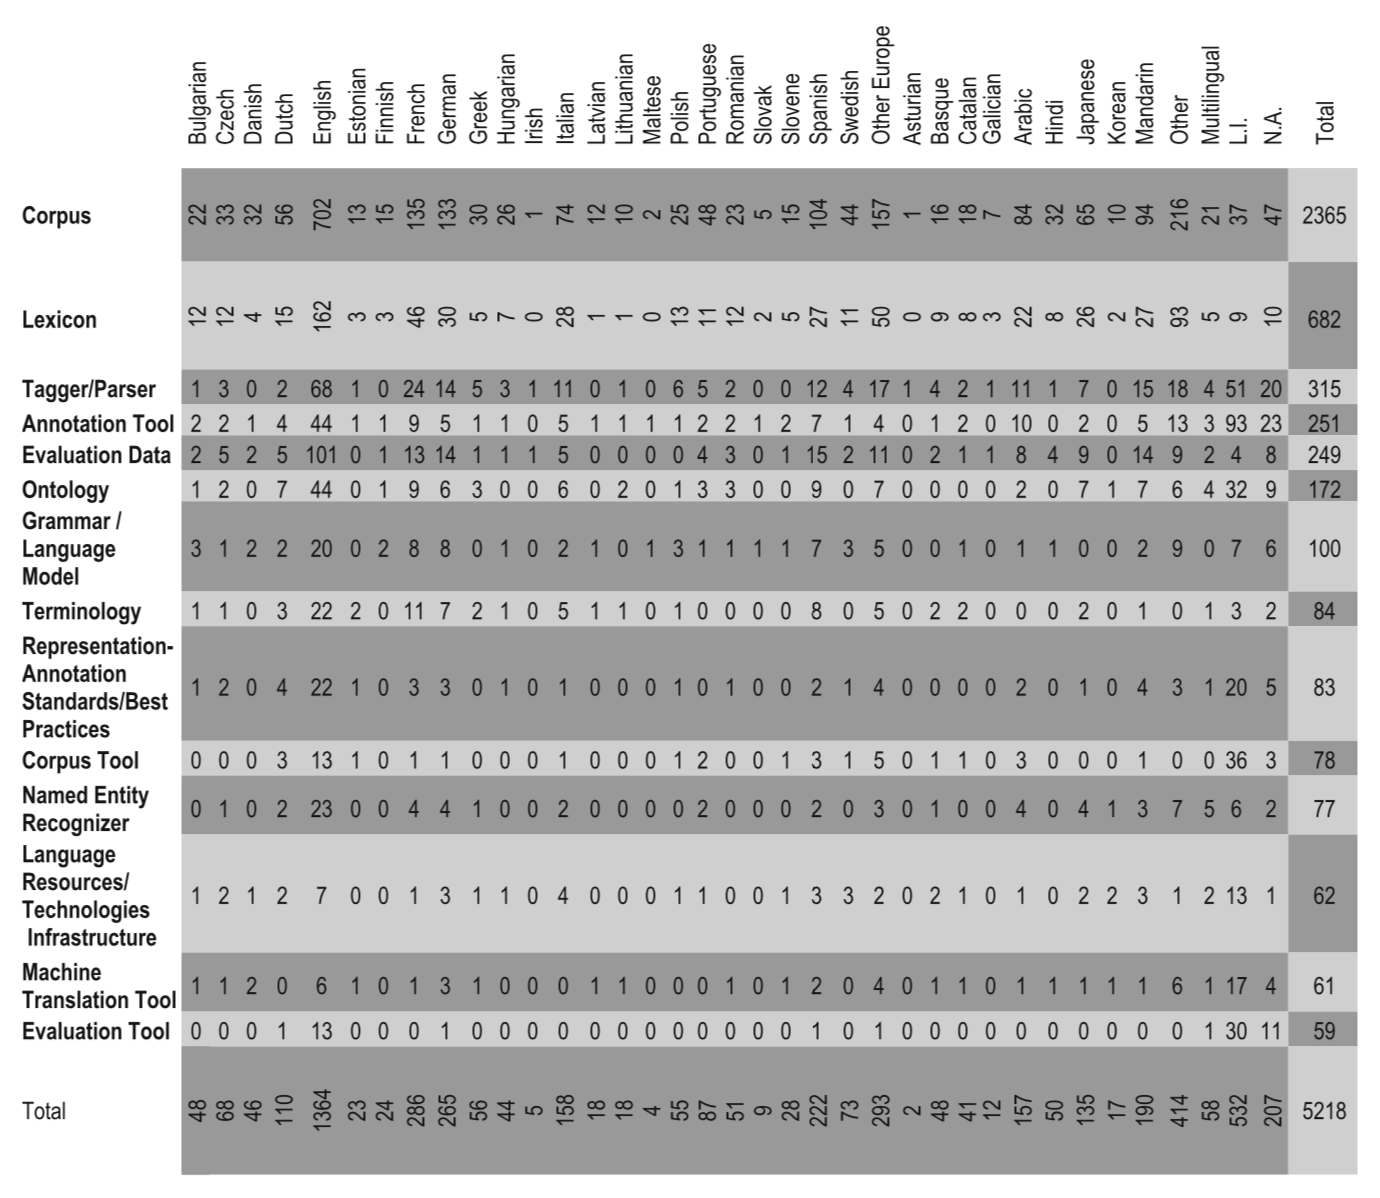
\includegraphics[width=1\textwidth]{img/lre.png}
 \caption{LRE maps for high resource languages \citep[460]{mariani2015language}}
 \label{fig:lre}
\end{figure}

Several authors working on LRE maps are also authors of the \citet{soria2017digital} paper; extending the LRE maps for low resource languages, and then intensifying efforts to develop low-hanging fruit for low resource languages is a logical next step for this research. The focus on European languages is expected; this may stem from the fact that LREC, the main conference series from which LRE data was drawn, is run by the European Language Research Association (ELRA). This fragmentation of the field is unsurprising, and happens in the reverse, as well: for example, \citet{paricio2010new} cites a framework for upgrading low resource languages which is explained in a research paper written in Spanish, and, anecdotally, around half of the papers presented at the Ryukyuan Heritage Language Society's conference in Tokyo in 2012 (which I attended) were presented in Japanese. This is not to say that fragmentation and diversity of linguistics in academia is something to be avoided, but rather that it is a hurdle to be noted and worked with to avoid repeated work and splintered efforts.

%\subsection{The current state of language diversity}
%
%In this section, I am going to briefly go into detail about what diversity means for linguistics. This will be useful later for explaining how related languages can be used to bootstrap work in similar languages. For instance, Irish spell-checkers and constitutional corpora from the EU can be used by Scottish Gaelic speakers with some tweaks in order to further improve their own systems.
%

\subsection{Who makes resources for languages?}
Another hurdle which was briefly alluded to earlier was the plethora of large organisations, databases, or projects dedicated to cataloguing low resource languages. Each of these has differences in scope, funding, and incentives. However, large organisations are not the only groups working on language development, digital ascent, language revitalisation, or any other shared focus that relates to low resource languages.

As \citet{hammarstrom2015unesco} points out, "language documentation and description is an extremely decentralized activity, carried out by missionaries, anthropologists, travellers, naturalists, amateurs, colonial officials, ethnographers and not least linguists over several hundred years." Language communities, amateur and professional linguists, educators, and language policy setters are most often involved in standardising a language and helping to document and revitalise low resource languages. Digitally, amateur computational linguists, and coders who are first language speakers of their own language are often the first to work on translating or migrating resources; this group is also often the first to set up Wikipedias in a local language (although this often leads to enthusiastic loners working outside of the main language communities) \citet{soria2017digital}. Beyond these groups, universities, local governments and businesses can also often develop language resources for low resource languages, as was the case with \citet{rognvaldsson2009icelandic}. After these groups, large grant-driven institutions such as CLARIN or the NSF fund a large portion of language development, along with industry giants such as Google or Xerox, and large military research arms such as DARPA.

Unfortunately, the lion's share of the overall funding for language development goes to languages which are already resourced.

\begin{quote}
Over the years the EU has invested massively in the development of language and speech technology, and many dedicated R\&D programmes have had a significant impact on its advancement, including applications oriented towards solving the multilinguality problem... Unfortunately the strong industrial bias of recent EU programmes has led to a situation where the major part of the funding for language and speech technology goes to the major languages. This is not surprising, as industrial players will prefer to invest in the development and deployment of technologies for larger markets. As a consequence there has been only marginal support for the development of language and speech technology for the language communities that do not constitute profitable markets. As the development cost of such technologies is independent of the number of speakers of a language ("all languages are equally difficult") this has created a very unbalanced situation. \citep{krauwer2006strengthening}
\end{quote}

Or:

\begin{quote}
Were it not for the special attention DARPA, one of the main sponsors of machine translation, devoted to Haitian Creole, it is dubious we would have any MT aimed at this language. There is no reason whatsoever to suppose the Haitian government would have, or even could have, sponsored a similar effort \citep{spice}. \citep[9]{kornai2013digital}
\end{quote}

Another good example of where funding and incentives for language development can be controversial would be Ethnologue, which rate limits and has a paywall guarding usage of their database, even though they are widely recognised as one of the best informed databases for language data. SIL International also gatekeeps the standard ISO 639-3, which is the most widely used language code. By having a paywall on their data, they exclude the general public from having control of codes for their own languages. SIL has also come under criticism for their Christian missionary work, as it can be viewed as complicit in culture change, and by extrapolation, ethnocide \citep{dobrin2009sil, dobrin2009practical, everett2009don}. This is just one example - and most likely one of the most extreme, not counting military work on languages used by insurgents in wars - of how organisations working on language resources may influence the work itself.

The funding of language resource development matters, because the way that the language community approaches language development affects the chance of survival for the language. This is one of the reasons that \citet{grenoble2016response} pointed out that "language vitality" is a more politically correct term to use than "language endangerment", as it takes the focus away from loss and focuses attention on language ascent. Another reason that language funding matters is because the major players with funding will generally be able to out manoeuvre smaller groups with different resources. This can enforce language shift, and can render resources created by individual developers moot. For instance, the secwepemc-facebook\footnote{\href{https://github.com/kscanne/secwepemc-facebook}{https://github.com/kscanne/secwepemc-facebook}} tool developed to automatically translate Facebook into low resource languages, created by the developer Neskie Manuel for his native Secwepemcts\'in, is no longer an active project and has not been updated, rendering it obsolete with Facebook UI changes, while automatic translation is provided for high resource languages natively by Facebook. Scannell, who helped port the secwepemc-facebook tool to Greasemonkey, was one of the authors of \citet{streiter2006implementing}, which suggested that developers for low resource languages use open source software pools in order to pool resources to enable them to overcome this - among other - issues facing low resource languages in particular.

% TODO Mention Bill and Melinda Gates foundation http://www.u.arizona.edu/~cashcash/aildi_2007/draftpt1_TELR2006.pdf
% TODO Mention Rosetta Stone https://www.rosettastone.com/endangered/projects
% TODO Mention FirstVoices and Canada https://fv.nuxeocloud.com/
% TODO Mention private companies: http://elalliance.org, living tongues, and http://terralingua.org, http://www.ogmios.org/index.php

As in Section~\ref{subsubsec:response}, covering all of the potential issues with funding and the politics of language development is well beyond the scope of this paper. However, focusing on how open source can help low resource languages is not. But first; what do I mean by "open source"?

% Here, I will explain briefly who makes language resources for these languages. I'll explain what I see as the main groups doing this work: professional translators, educators, missionaries (of multiple faiths, but mostly Christian), academics and native technologists. I'll explain each stakeholder and their canonical perspectives.

% Alexis: what do you mean by "their canonical perspectives"? will this section address creation of digital resources only, or all resources? for that matter, what counts as a digital resource? does a collection of pdf scans of old books count? how about a pdf version of a text collection? etc....
% I don't immediately see how this fits into the rest of the thesis. also look at relevant publications from Jeff Good - one in particular on the ecology of language documentation: http://www.acsu.buffalo.edu/~jcgood/publications.html


%\subsection{Language research funding}
%
%Here, I'll go into more depth about funding, as we've outlined who works on LRLs and who would fund research, and why. This will further inform the basis for the work of the previous section. I'll talk about DARPA MT funding in the 20th century, as well as other efforts such as CLARIN.



% IARPA and DARPA both are involved with low resource languages and both of them may have their own institutional values that are probably at ends with independent researchers, commercial consumers, and language communities. Does working on sparse data openly bring along with it ethical or moral concerns; if so, how can these be adequately explained, breached, and talked about? How can they be worked around or be part of the conversation? Note that DARPA and the like also use humanitarian reasons as their primary stated aim for work on sparse languages, which may be contrary to their military needs. There is already an extensive literature on moral uses of data -- I could summarize that, and apply it specifically to low resource languages, which is something I do not think has yet been published.

% Darpa: http://www.darpa.mil/program/low-resource-languages-for-emergent-incidents
% IARPA: http://www.iarpa.gov/index.php/research-programs/babel

% - Institutional bottleneck
% - Linguistic colonialism
% - Ethical and moral concerns for military usage
% - Ethical and moral concerns for big business usage



%% TODO include this, formerly in introduction

%Incidentally, there is something to be said for spoken language corpora, which may be more prevalent in some cases than written resources (especially in a region with a history of radio transmissions in the local language, for instance). However, the direct use of spoken language corpora for building language resources is limited and generally requires more processing and development time (not to mention storage), compared to cheap, written data.
% Alexis: also what about spoken language corpora? e.g. work by Oliver Adams & colleagues inducing linguistic information from spoken data, skipping the usual transcription set. I'm not saying you need to also deal with spoken language data, but it does need to be acknowledged

% TODO Where do we mention ILAT? http://www.u.arizona.edu/~cashcash/ILAT.html
% !TEX root = thesis.tex
\section{Open Source Code}
\label{sec:open-source}

{\it Open Source} is a complex concept which can refer to any code that is permissively licensed, not just code related to computational linguistics. Here, I will define what I mean by Open Source. This will largely inform the next section where I talk about its use for low resource languages.

\subsection{Defining {\it open source}}
\label{subsec:defining-open-source}

At its core, {\it open source} refers to code which has a license which allows it to be freely inspected, used, or modified by anyone, without restriction. The concept was introduced in 1998 by Linux programmers such as Eric Raymond, author of {\it The Cathedral and the Bazaar}\footnote{\href{http://www.catb.org/~esr/writings/cathedral-bazaar/}{http://www.catb.org/~esr/writings/cathedral-bazaar/}. \last{May~2}} \citep{raymond1999cathedral}; Linus Torvalds, author of the Linux kernel\footnote{\href{https://www.kernel.org/}{https://www.kernel.org/}. \last{May~2}} and Git\footnote{\href{https://git-scm.com/}{https://git-scm.com/}. \last{May~2}}; Richard Stallman, founder of the GNU project\footnote{\href{https://www.gnu.org/}{https://www.gnu.org/}. \last{May~2}} and the Free Software Foundation\footnote{\href{https://www.fsf.org/}{https://www.fsf.org/}. \last{May~2}}; and others in response to the Netscape browser's code being openly licensed and made available.

{\it Open source} is one of many terms which can be used to differentiate code which is either available or licensed permissively for re-use; other terms include {\it free} and {\it libre} software. There is no standard definition of open source that is universally accepted.

Nor will universal acceptance be forthcoming. The issue regarding reconciliation between open source, free software, and the rest of the terms stems largely from a difference of opinion between what constitutes open software, and what free and open means. An oft-used expression is "free as in beer" as opposed to "free as in speech", where the first is used for gratis software which has no monetary price set on it, and the second is used to refer to software which is written without restriction. The term {\it libre} is most often used for this second definition, to differentiate the two meanings in English. Occasionally, the acronym FLOSS is used in open source parlance to refer to Free Libre Open Source Software, which is both gratis and libre software.

For some adherents, software ought to be free (gratis), as it is a result of human labour and because opening it up without cost maximises the potential usefulness of that code, and minimises duplicated effort. This idea contains harks back to the idea of a digital commons: like the commons in philosophical and economic literature (cf. \citepos{hardin2009tragedy} seminal article on the subject), code can be viewed as a resource that belongs to humanity as a whole, and not the creators who initially fashioned it. In this sense, open source is a more of a philosophical theme than a technical term.

\begin{quote}
Open source is a development methodology; free software is a social movement. For the free software movement, free software is an ethical imperative, essential respect for the users' freedom. By contrast, the philosophy of open source considers issues in terms of how to make software  "better" - in a practical sense only. It says that nonfree software is an inferior solution to the practical problem at hand.\footnote{\href{https://www.gnu.org/philosophy/open-source-misses-the-point.html}{https://www.gnu.org/philosophy/open-source-misses-the-point.html}. \last{May~2}}
\signed Richard Stallman (Founder of GNU\/Linux)
\end{quote}

However, for the most part, open source is not disambiguated as a term, because authority for this task is delegated to the license put on a piece of software, which determines the legality and potential use. Licenses determine the legal rights to sharing code. A piece of code which is taken from a proprietary server and published on the internet is not necessarily open source. In this instance, the code may have been illegally copied and shared, but it is not licensed for free usage. Under no definitions is this considered open source. Indeed, this touches upon issues of digital copytheft and piracy, which is a standard term used frequently in the media and in legal proceedings to attach a sense that copying code is the same as larceny or theft on the high seas. Avoiding the question of the validity of this viewpoint, it is important to focus on the license as the differentiating factor between code which has been released legally under an open definition or not. The term open source under most definitions does not pertain to ethical concerns about the software's usage, but rather simply refers to whether or not it is permissively licensed and available for users.

There are many licenses which are considered to be open source, and there are several arbiters available which judge the validity of open source licensing. The Open Source Initiative (OSI) maintains a list of approved licenses on their website.\footnote{\href{https://opensource.org/licenses}{https://opensource.org/licenses}. \last{May~2}}

The OSI, whose founders were one of the original coiners of the term {\it open source}, has several parameters by which open source software can be judged as being `open' or `closed' (that is, proprietary, non-permissively licensed, non-reusable, limited in usage to a set amount of people, and so on). It may be useful to list these terms directly below, as they are instructive about how open source can be a nuanced term. These terms and their definitions are from the OSI's website,\footnote{\href{https://opensource.org/osd}{https://opensource.org/osd}. \last{May~2}} and are repeated below verbatim.

\begin{enumerate}
\item{Free Redistribution}. The license shall not restrict any party from selling or giving away the software as a component of an aggregate software distribution containing programs from several different sources. The license shall not require a royalty or other fee for such sale.
\item{Source Code}. The program must include source code, and must allow distribution in source code as well as compiled form. Where some form of a product is not distributed with source code, there must be a well-publicized means of obtaining the source code for no more than a reasonable reproduction cost, preferably downloading via the Internet without charge. The source code must be the preferred form in which a programmer would modify the program. Deliberately obfuscated source code is not allowed. Intermediate forms such as the output of a preprocessor or translator are not allowed.
\item{Derived Works}. The license must allow modifications and derived works, and must allow them to be distributed under the same terms as the license of the original software.
\item{Integrity of The Author's Source Code}.
  The license may restrict source-code from being distributed in modified form only if the license allows the distribution of "patch files" with the source code for the purpose of modifying the program at build time. The license must explicitly permit distribution of software built from modified source code. The license may require derived works to carry a different name or version number from the original software.
\item{No Discrimination Against Persons or Groups}.
  The license must not discriminate against any person or group of persons.
\item{No Discrimination Against Fields of Endeavor}.
  The license must not restrict anyone from making use of the program in a specific field of endeavor. For example, it may not restrict the program from being used in a business, or from being used for genetic research.
\item{Distribution of License}.
  The rights attached to the program must apply to all to whom the program is redistributed without the need for execution of an additional license by those parties.
\item{License Must Not Be Specific to a Product}.
  The rights attached to the program must not depend on the program's being part of a particular software distribution. If the program is extracted from that distribution and used or distributed within the terms of the program's license, all parties to whom the program is redistributed should have the same rights as those that are granted in conjunction with the original software distribution.
\item{License Must Not Restrict Other Software}.
  The license must not place restrictions on other software that is distributed along with the licensed software. For example, the license must not insist that all other programs distributed on the same medium must be open-source software.
\item{License Must Be Technology-Neutral}.
  No provision of the license may be predicated on any individual technology or style of interface.
\end{enumerate}

\subsection{Open source licenses}
\label{subsec:licenses}

The different terms and conditions listed above are often conflated, and a legally-valid license which satisfies all of them is difficult to write on an {\it ad hoc} basis. For this reason most open source programming relies on using existing licenses, and copying them for specific projects. There are tools today to help make licensing more clear to na\"ive users, such as \href{https://choosealicense.com}{choosealicense.com}, \href{https://tldrlegal.com}{tldrlegal.com}, and so on.

Some of the main licenses used in the wild are as follows:

\begin{itemize}
\item The X11 license, developed at MIT and more commonly called the MIT license,\footnote{\href{https://www.gnu.org/licenses/license-list.en.html}{https://www.gnu.org/licenses/license-list.en.html}. \last{May~3}} is the most popular license on Git\-Hub,\footnote{\href{https://github.com}{https://github.com}. \last{May~2}} the world's largest repository of code. It is used in over 40\% of the projects licensed there as of March 2015\footnote{\href{https://blog.github.com/2015-03-09-open-source-license-usage-on-github-com/}{https://blog.github.com/2015-03-09-open-source-license-usage-on-github-com/}. \last{May~2}}, and in almost a million projects indexed by the package indexer at \href{https://libraries.io}{\nolinkurl{libraries.io}}.\footnote{\href{https://libraries.io/licenses}{https://libraries.io/licenses}. \last{May~3}} It is a very permissive license, which allows commercial use, modification, distribution, sublicensing, and private use of any code so licensed. It also waives liability for the authors of the code, saving them from needing to worry about lawsuits in cases where their code would otherwise be liable - the code is granted as is, and what the user does with it is not the author's fault. The only restriction is that you need to include the license in any software which uses it.
\item The Apache License 2.0, developed by the Apache Software Foundation,\footnote{\href{https://www.apache.org/licenses/}{https://www.apache.org/licenses/}. \last{May~2}} is similar, but disallows users from trademarking code with the license, requires a few smaller modifications like stating code changes and adding a NOTICE file, if one exists, to derivational code, and also adds a patents clause for contributors.
\item The BSD licenses were developed for use with Berkeley Software Distribution, a Unix-like OS. There have been multiple iterations; the first, 4-clause license required every subsequent license to reference and acknowledge the original, ending with large lists of acknowledgements; a subsequent 3-clause license (often called the "New" BSD) removed this, but kept a clause which stated that usage does not imply endorsement by the original contributors; and this was removed in a 2-clause version, often called "Simplified" or the "FreeBSD" license.
\item The GNU General Public License (GPL)\footnote{\href{https://www.gnu.org/licenses/}{https://www.gnu.org/licenses/}. \last{May~2}} is the main example of copyleft licensing, where any derivative works that use GPL licensed code must also use a GPL license. This causes major issues when users want to combine code from multiple sources, some of whose licenses may conflict. For this reason, the GNU Library or "Lesser" General Public License (LGPL) was created, to allow only code under the LGPL to be accessible and modifiable openly, while all other code does not have to be. GPL also demands that users include installation instructions,
\item Creative Commons licenses,\footnote{\href{https://creativecommons.org/licenses/}{https://creativecommons.org/licenses/}. \last{May~2}} mostly used for sharing non-code material such as images and documents openly, was created by Lawrence Lessig, the founder of the Creative Commons organisation,\footnote{\href{https://creativecommons.org/}{https://creativecommons.org/}. \last{May~2}} and may also be used for code projects. There are many licenses they offer, and some variants are copyleft licenses - in particular, "share-alike" clauses are an example of copyleft.
\item The Unlicense,\footnote{\href{https://unlicense.org/}{https://unlicense.org/}. \last{May~2}} created in 2010, is another option, which explicitly states that code is unlicensed, with no restrictions, and also with no liability for the authors (unlike code which is not licensed, which has stricter protections under US copyright law than code which specifically excludes a license). There is a Creative Commons Zero,\footnote{\href{https://creativecommons.org/publicdomain/zero/1.0/}{https://creativecommons.org/publicdomain/zero/1.0/}. \last{May~2}} license which is similar, as well as the WTFPL license ("Do What The Fuck You Want Public License")\footnote{\href{http://www.wtfpl.net}{http://www.wtfpl.net}. \last{May~2}} which, although intentionally comically profane, is non-trivial in that it is used in 11,714 different software projects on GitHub as of this writing.\footnote{\href{https://github.com/search?q=license\%3AWTFPL}{https://github.com/search?q=license\%3AWTFPL}. \last{May~2}}
\end{itemize}

As is clear from these short descriptions, licenses are not easily interchangeable and they come with a range of suppositions about how the data ought to be used. Copyleft licenses (mostly GPL) require any derivative works to also be open source, which means that they cannot be used in proprietary codebases, leading to fragmentation of the code space and to legality issues in the long run. However, the effects of copyleft may be more perfidious, in that funders or developers may avoid projects altogether if they find a project has (or does not have) a copyleft license. The same could be said for liability waivers, or more especially the lack thereof. This is backed up in studies: for instance, two thirds of respondents for GitHub's open source survey in 2017 said that they value licensing as a major factor when contributing to a project.\footnote{\href{http://opensourcesurvey.org/2017/}{http://opensourcesurvey.org/2017/}. \last{May~2}} Ultimately, licenses are complicated legal documents with various repercussions for how code is accessible.

\subsection{Where is open source code?}
\label{subsec:where-is-open-source-code}

For closed source or proprietary software, the code itself often is not stored in the open or accessible to third parties. However, for open source software to be defined as open source according to OSI's definitions, it needs to be publicly accessible and well-publicised. This means that storing code on a server where it could technically be accessed via some protocol, or less ideally through a mail-order CD as \citet{krauwer2006strengthening} suggested, is not enough; instead, it ought to be linked to elsewhere and available for everyone to access. This raises the question: where is most open source code stored?

Unequivocally, GitHub\footnote{\href{https://github.com}{https://github.com}. \last{May~2}} is the largest source of shared, open code on the internet, with 27 million users and 80 million repositories\footnote{Not all of the projects  included in these numbers are public.} as of March 2018.\footnote{\href{https://github.com/about}{https://github.com/about}. \last{May~2}} There have been several large-scale studies of its codebase by researchers \citep{gousios2012ghtorrent, allamanis2013mining, gousios2014lean, kalliamvakou2014promises, beller2016analyzing} which confirm this. Other large repositories for code of a similar nature, include Sourceforge, with 430k projects and 3.7m users,\footnote{\href{https://sourceforge.net/}{https://sourceforge.net}. \last{April~18}} Bitbucket\footnote{\href{https://bitbucket.org/}{https://bitbucket.org/}. \last{May~2}} with 5m users,\footnote{\href{https://blog.bitbucket.org/2016/09/07/bitbucket-cloud-5-million-developers-900000-teams/}{https://blog.bitbucket.org/2016/09/07/bitbucket-cloud-5-million-developers-900000-teams/}. \last{May~2}} Launchpad\footnote{\href{https://launchpad.net/}{https://launchpad.net/}. \last{May~2}} with 4.2m users,\footnote{\href{https://launchpad.net/people}{https://launchpad.net/people}. \last{May~2}} and Gitlab,\footnote{\href{https://about.gitlab.com/}{https://about.gitlab.com/}. \last{May~2}} which holds the majority share of self-hosted Git platforms.\footnote{\href{https://about.gitlab.com/is-it-any-good/}{https://about.gitlab.com/is-it-any-good/}. \last{May~2}} All of these platforms are based around Git, the versioning software developed by Linus Torvalds, used to store different versions of code for developers and teams, which lends itself particularly to shared code that can be updated easily by outside and community developers. (`Repository' is a term for a single Git instance, equatable with a single project.)

Self-hosted Git instances are a common way of storing proprietary code; one sets up a versioning system within a company, using the tools and set of social standards that developers are used to from working on open source code, but limit access to employees. This is what is meant by GitLab's statement that they host most self-hosted Git platforms. Git is not the only possible versioning software for this; Google has their own versioning tool, Piper, which hosts the over two billion lines of code used by the majority of the company in a single repository.\footnote{\href{https://www.wired.com/2015/09/google-2-billion-lines-codeand-one-place/}{https://www.wired.com/2015/09/google-2-billion-lines-codeand-one-place/}. \last{May~2}} Self-hosted Git instances are generally not open source. Generally, if someone wants to use a shared Git repository, they are limited to paying a fee for a hosting service, or using sites that have a freemium model where public repositories are free, but private or enterprises instances are not.

There are alternatives to cloud storage (the `cloud' here being a common metaphor for hosting on someone else's servers) with a hosting provider; one would be storing the code on your own website, and running your own server or building the user interface yourself. This is largely uncommon due to setup costs, but occasionally happens with academics and smaller teams who are not used to larger hosts or who are worried about the longevity of providers. This latter worry is founded; for instance, Google Code\footnote{\href{https://code.google.com/archive/}{https://code.google.com/archive/}. \last{May~3}} was closed after ten years of running in 2016, causing many projects to need to port to another service such as GitHub. For academics, a common solution to offset setup and hosting costs is to use university websites and archives as a suitable place to store open source code. For instance, Giellatekno, a language-technology research group, and Divvun, a linked product development group, both work primarily on S\'ami languages, and both use the same Subversion (another versioning system) database for storing their code \citep{moshagenopen}, which is hosted by UiT The Arctic University of Norway.\footnote{\href{http://giellatekno.uit.no/}{http://giellatekno.uit.no/}. \last{May~2}}

In a large part, the question of where to store information - especially academic information regarding languages - is one which the large archival sites mentioned in Section~\ref{subsec:finding-resources} were created to solve. In particular, this is true for non-code resources, such as audio and video corpora, which historically have been prioritised for storage over code due to the size and relative importance of the corpora, and due to the older industry standards of keeping all code related to research private, especially when that code was funding by enterprise. Many of these sites are repositories of metadata which pointed to individually hosted content, which made the links susceptible to link rot and offloaded the issue of storage altogether.

Today, however, there is a sea change towards putting computational work in the open. Occasionally, this means that academics point to the open source code for their papers on GitHub or elsewhere, or publish their software itself as a research object. For example, \citet{makela2016integrated} and \citet{kleinberg2017web} were published with the Journal of Open Source Software (JOSS)\footnote{\href{http://joss.theoj.org/}{http://joss.theoj.org/}. \last{May~2}} \citep{smith2018journal}, which peer-reviews, publishes, and assigns digital object identifiers (DOIs) to software as a way of recognising important academic work. The code for these papers is publicly available on GitHub. Incentivising academics to publish their code openly is difficult, as software is not weighted in job reviews the same way as research papers; however, there are other benefits such as reproducibility and transparency. There are efforts to align these incentives; for instance, The Austin Principles of Data Citation in Linguistics \citep{AustinPrinciples2017} was created to emphasise the importance of citing, using, and storing linguistic data properly. Standardising open source paradigms in academia is an ongoing work.

\subsection{Digital permanence and storage}
\label{subsec:digital-permanence}

Focusing a bit closer on the academic use case, we can easily imagine a case where a professor puts code related to research on a university server, only to see that server change hands, go offline, or become defunct if the professor leaves the university for a position elsewhere or if their focus changes. This is more true of graduate students, who do not have the same locational longevity as staff. As mentioned briefly above, this can lead to link rot; links which formerly pointed to workable software may then point nowhere or to the wrong resource. Links can also be improperly shared; for instance, some websites may have improper subdomain settings leading to an inability for the website to resolve if not typed specifically.\footnote{For example, {\tt resourcebook.eu/searchll.php} does not resolve, but {\tt http://www.resourcebook.eu/searchll.php} does. This lead me to mistakenly believe that \citepos{calzolari2012lre} website was down for several weeks.}

These are artefacts of systemic defects; in a location-based protocol (such as the Hypertext Transfer Protocol (http) protocol used by most websites today), consistency of location is prioritised over consistency of content. If the content was pointed to using some more permanent reference, such as a DOI, than the object could be moved without issues, and the problem of link rot is largely solved.

Digital permanence is a larger issue than code placed in locations by individual actors, however. Large organisations may lose their funding, come to the end of their expected lifecycle, or decide to shutter or obfuscate projects upon which research or language communities may depend. A good example would be Google Code, mentioned above in Section~\ref{subsec:where-is-open-source-code}. Another example might be listserv.heanet.ie,\footnote{\href{https://listserv.heanet.ie}{https://listserv.heanet.ie}. \last{May~2}} which probably held the largest corpus of Irish data at one point, but which was unavailable to crawlers and depends upon the hosting of heanet.ie for continued service \citep{scannell2007crubadan}. A final example might be the linguistic vitality database by Kornai's group mentioned earlier,\footnote{\href{https://hlt.bme.hu/en/projects/lingvit}{https://hlt.bme.hu/en/projects/lingvit}. \last{May~2}} which is is currently in stasis pending funding (Kornai personal communications, 2018).

Aside from the problem of code actively being stored, there is another issue with code rot. Over time, the ecosystem around which code is built changes, and it becomes harder to reproduce the original environment where code was installed and executed, leading to the code itself becoming less useful \citep{eide2010toward}. Some solutions to this problem involve using containers like Docker to emulate the original environment \citep{boettiger2015introduction}. While this research has largely been driven by a need to replicate scientific results \citep{schwab2000making, barnes2010publish, ince2012case}, it is also relevant outside of academic research to enterprise and community solutions to difficult coding problems, such as natural language processing.

As computational languages naturally evolve, it is important to take into account that the code must also be maintained if it is going to find consistent usage. Maintenance is a difficult task that has few immediate incentives, and which generally involves long timelines. It involves not only solving bugs as they appear with general usage, but also ensuring that the code stays relevant in a changing ecosystem. No package exists or application exists by itself; each depends upon other code to run. This is especially true for software built using the Unix methodology of piecing together many small pieces of software that do one function well.\footnote{\href{http://www.catb.org/esr/writings/taoup/html/ch01s06.html}{http://www.catb.org/esr/writings/taoup/html/ch01s06.html}. \last{May~3}} Applications also depend upon code, though; as operating systems (OS) update, legacy maintenance is needed to ensure forward compatibility, or the code will become defunct as no one will be able to run it on current OSs. However, providing funding for maintenance at the OS timescale is exceedingly difficult.

% Note: I moved Data and Privacy to section 4, because I want to talk about LRLs specifically there, and this is more of an issue for LRLs. I deleted the old Licensing and Liability section, as I already mentioned it.

% Covered briefly below
% \subsection{Military and enterprise solutions}
% \label{subsec:military-and-enterprise}
% In this section, I will talk about how open source meshes with military and enterprise development.

\subsection{Funding}
\label{subsec:oss-funding}

Open source code cannot by definition be sold directly for a profit; open source code must be freely available to all users. This raises an issue where funding for open source development is not direct in the sense of immediate fiscal returns. In this business environment, other funding models need to be pursued. The obvious, most common solution is to sell services on top of open source code, and give away the code itself for free. There are benefits to doing this. Giving away code can be seen as a marketing tactic, drawing other developers, or it may serve to develop a community of active developers who are interested in giving back to the original project without being employed by the core developer's company, or it may serve as a retention device keeping in-house developers who prefer to work in the open happy, or it may serve as a way of verifying a level of security for the code itself, by allowing other participants to point out flaws in the system and fix them without needing to rely upon expensive and possibly ineffectual internal security audits.

For researchers, open sourcing code can be seen as a major time investment \citep{fitzjohn2014reproducible, lowndes2017our}, and although it can help reproducibility, it is not normally the primary source of sharing research (which would be the scientific article). For researchers, funding needs to come from either salaries, from the researcher's free time, or from grants from larger institutions (not counting enterprise and interdisciplinary cross-overs). This is a serious barrier to open source work in the sciences.

For militaries and governments, there is little incentive to open source unless there is a direct mandate from their political constituents or legal process. Even when there are open challenges run by military branches - for example, the DARPA-sponsored LORELEI challenge\footnote{\href{https://www.nist.gov/itl/iad/mig/lorehlt-evaluations}{https://www.nist.gov/itl/iad/mig/lorehlt-evaluations}. \last{May~2}} - there are often no demands that any resulting work be open sourced (although the initial challenge is open sourced as a way of inviting participation). Often, this is because the code itself has security concerns; for example, open sourcing speech recognition software for languages spoken by military targets in lossy situations (such as over cell networks) would only illuminate that such software exists. This example of security through closed source methodologies extends to enterprise; for Google to open all of their MT data would cause them to lose a competitive edge in the translation market.

For software developers outside of academia, militaries, governments, and large enterprises that have business advantages, however, open sourcing code can be a significant way to gain prestige, to improve and market developer relations, to market themselves to prospective clients and companies, and to contribute to their coding communities. There are a variety of ways of funding work within the open source model.

One direct way is to add payment schemes directly to source code or to a website, asking for donations. Another would be to use a collective community to allocate donations and funds; Open Collective\footnote{\href{https://opencollective.com/}{https://opencollective.com/}. \last{May~2}} is an example of a company that helps do this for developers, some of whom are paid entirely through funds on the site.\footnote{\href{https://medium.com/open-collective/a-new-way-to-fund-open-source-projects-91a51b1b7aac}{https://medium.com/open-collective/a-new-way-to-fund-open-source-projects-91a51b1b7aac}. \last{May~2}} Crowdfunding sites can also be useful for some developers. Patreon is a good example where makers can earn money directly through fan donations, while Kickstarter has been used many times to fund projects. For example, Dave Gandy, the developer for Font Awesome, an open source font resource, raised over a million dollars in a month from 35,550 backers for the next version of his product.\footnote{\href{https://www.kickstarter.com/projects/232193852/font-awesome-5}{https://www.kickstarter.com/projects/232193852/font-awesome-5}. \last{May~2}} Code bounties, funds set by community members hoping to have other developers solve bugs, is another limited way of making money.\footnote{\href{https://www.bountysource.com/}{https://www.bountysource.com/}. \last{May~2}} Cryptocurrencies may eventually present other ways of funding open source, either directly,\footnote{\href{https://utopian.io/}{https://utopian.io/}. \last{May~2}}\footnote{\href{https://gitcoin.co/}{https://gitcoin.co/}. \last{May~2}} or through other avenues like initial coin offerings. Already, some companies are using initial coin offerings (similar to IPOs in the business world, but instead marking the launch of a new cryptocurrency) to fund development on open source, such as with Filecoin, which raised over 200 million for their coin development, of which many of the funds will go directly to open source projects run by the company Protocol Labs, such as IPFS \citep{benet2014ipfs} on GitHub.\footnote{\href{https://coinlist.co/filecoin}{https://coinlist.co/filecoin}. \last{May~2}}

There are several guides online that outline other ways of funding open source.\footnote{\href{https://github.com/nayafia/lemonade-stand}{https://github.com/nayafia/lemonade-stand}. \last{May~2}}\footnote{\href{https://medium.com/open-source-life/money-and-open-source-d44a1953749c}{https://medium.com/open-source-life/money-and-open-source-d44a1953749c}. \last{May~2}}\footnote{\href{https://opensource.guide/getting-paid/}{https://opensource.guide/getting-paid/}. \last{May~2}} In the end, the majority of open source developers are not remunerated for their work directly. Most open source work is unpaid, and maintenance of open source software can be demanding and costly for developers who do not set expectations around levels of support for users. This is especially difficult for developers who do not have total control of their projects, such as is often the case with developers doing open source within a company.

More specifically, the problem of funds being directed to low resource languages is unlikely to be solved by any of the proposed solutions above. However, by banding together and sharing tools openly \citep{streiter2006implementing}, computational linguists working on low resource languages can expedite their work. This methodology will be explored in Chapter~\ref{sec:lrl-code}.

\subsection{Non-English programming languages}

\setcode{utf8}

So far, there has been no mention of coding itself happening in languages besides English. The vast majority of the open source world uses English in documentation of code resources and in the code language itself. The first is self-explanatory; for the second, take for example the common tokens `if` and `else`, used in conditionals. These could be written in another language, as they are English words, or in another script, such as Arabic. However, this is rare. There are some cases of programming languages themselves being written in other languages, such as \< قلب > (Qalb), which is written in Arabic.\footnote{\href{http://qlb-repl.herokuapp.com/}{http://qlb-repl.herokuapp.com/}. \last{May~3}} For Qalb, the popular `hello world' command would be written:

\begin{arabtext}
(قول "مرحبا يا عالم"‏)
\end{arabtext}

More commonly, coding in another language means using translations of very popular libraries documentation. For instance, the Node.js\footnote{\href{https://nodejs.org/}{https://nodejs.org/}. \last{May~3}} i18n committee\footnote{\href{https://github.com/nodejs/i18n/}{https://github.com/nodejs/i18n/}. \last{May~3}} is currently working on tools to translate the most popular JavaScript framework's documentation into a few popular languages, like Spanish and Portuguese. Often, these efforts depend upon bilingual volunteers, willing to translate documentation into another language.

The Online Historical Encyclopaedia of Programming Languages's website\footnote{\href{http://www.hopl.info/}{http://www.hopl.info/}. \last{May~3}} notes that the vast majority of languages were created in English speaking countries.\footnote{\href{http://www.hopl.info/countriesreportgr.prx}{http://www.hopl.info/countriesreportgr.prx}. \last{May~3}} For the most part, languages which are written in other languages do not have the same amount of reach or ecosystem size as languages developed in English. All of the top 15 languages on GitHub in 2017 were based on English.\footnote{\href{https://octoverse.github.com/}{https://octoverse.github.com/}. \last{May~3}}

That English is needed to code means that any coder wishing to developer resources in their native language will most likely need to use English or other major languages for the vast majority of the work. While solving this problem is out of scope here, it is worth mentioning this aspect of language resource development. There is active work in this field, both for high and for low resource languages; for instance, Lassi\footnote{\href{https://github.com/julienmalard/Lassi}{https://github.com/julienmalard/Lassi}. \last{May~3}} is a tool in development which allows Kaqchikel speakers to code entirely in their own language, by automatically translating code from one language to another.

% Note: I moved the entire section on ethics in open source to the Discussions chapter

% \subsection{Defining "open source"}
% \subsection{Where is open source code?}
% \subsection{Data rights and privacy}
% \subsection{Liability}
% \subsection{Funding}
% \subsection{Military and enterprise solutions}
% \subsection{Ethical reasons for using open source}
% !TEX root = thesis.tex
\section{Open Source Code for Low Resource Languages}
\label{sec:endlangcode}

Now that low resource languages (LRLs) have been described, and now that there has been a brief overview of open source as a software methodology, the reader will doubtless wonder - what is the state of open source code that can be used today by language communities?

Unfortunately, due to the decentralised nature of open source, this is an inherently difficult question to answer. In the ecosystem, there are a few strategies that can be used to inform an answer: use a specific task as a case study for what tools would be used, look at what resources are available from any of the main large data aggregators mentioned in Section~\ref{subsec:resource-aggregators}, take a screenshot of the ecosystem based on some of the more-cited open source tool used for LRL NLP, examine linked open data, and sample relevant work on GitHub through a manually collected list of resources. Each of these strategies is employed in a subsection, below.

\subsection{Case study: Mapping linguistic co\"ordinates}

The breadth of HLT is wide; choosing a specific task within it and then trying to perform that task as adequate as possible would be one way to figure out how much open source code exists, and what that looks like. For example, suppose we were interested in making dialect maps using language co\"ordinates. This is an old research area in linguistics \citep{trudgill1983on,labov2005atlas}, and computational methods for mapping languages have been described in some research, including in the recently started {\it Journal of Linguistic Geography} \citep{labov2012journal}.

For NLP, this is a nontrivial task. Language maps using geolocational data could be used in several ways. For instance, \citep{mccrae2015reconciling} mentions an email sent to the {\it Corpora List} asking for "freely available geotagged tweets collection for research purpose."\footnote{\href{https://mailman.uib.no/public/corpora/2015-February/022044.html}{https://mailman.uib.no/public/corpora/2015-February/022044.html}. \last{April~26}} Geolocation can also be used to plot language relatedness \citep{littauer2012visualizing}.

Another example where geolocation might be useful would be in l10n in the browser. For instance, if the client's browser does not send a {\tt Accept-Language} header\footnote{\href{https://tools.ietf.org/html/rfc7231\#section-5.3.5}{https://tools.ietf.org/html/rfc7231\#section-5.3.5}. \last{April~27}} in their requests to view a website, specifying languages the client understands by using ISO 639 tags\footnote{\href{https://www.ietf.org/rfc/bcp/bcp47.txt}{https://www.ietf.org/rfc/bcp/bcp47.txt}. \last{April~27}}, then the server may use the {\tt Navigator\-Language} object in JavaScript\footnote{\href{https://www.w3.org/TR/html51/webappapis.html\#language-preferences}{https://www.w3.org/TR/html51/webappapis.html\#language-preferences}. \last{April~27}} to query for the language of the browser UI (normally set by the users depending on where they downloaded it), or they could ask the browser directly through the geolocation API (for instance, on Firefox\footnote{\href{https://www.mozilla.org/en-US/firefox/}{https://www.mozilla.org/en-US/firefox/}. \last{April~27}}\footnote{\href{https://developer.mozilla.org/en-US/docs/Web/API/Geolocation/Using_geolocation}{https://developer.mozilla.org/en-US/docs/Web/API/Geolocation/Using\_geolocation}. \last{April~27}}) to supply the geolocation of users and extrapolate plausible languages from this data. Knowing where the user is likely to be, and what languages the user is likely to prefer using, could help with providing their native language automatically in the browser.

\citet{gawne2016mapmaking} give a general overview of the mapping field currently, pointing out that the main resource for finding language geographical co\"ordinates comes from the World Language Mapping System\footnote{\href{http://www.worldgeodatasets.com/language/.}{http://www.worldgeodatasets.com/language/}. \last{April~25}}, a website owned and run by SIL, which are used for ISO 639-3 labelling, and by Glottolog and OLAC. The maps are under a closed license and must be purchased. \citet{gawne2016mapmaking} also mention WALS, which uses its own geographical co\"ordinates, and the ELP, which understandably uses Google Maps as its mapping program, and draws from multiple sources. They also mention Language Landscape,\footnote{\href{http://www.languagelandscape.org/}{http://www.languagelandscape.org}. \last{April~25}} a project which maps instances of language use on a map.

To use these geographic information systems (GIS), one needs to download licensed map data, which could be open or closed. Then, one has to have a mapping software to display that data. This software must also be appropriately licensed. Google Maps is not open source, although it is {\it open access}, in that it is free to use. An open source equivalent of Google Maps is Open Street Maps,\footnote{\href{https://www.openstreetmap.org/}{https://www.openstreetmap.org/}. \last{April~27}} a community built tool that is permissively licensed as CC-BY-SA.\footnote{\href{https://www.openstreetmap.org/copyright}{https://www.openstreetmap.org/copyright}. \last{April~27}} One could use data from Glottolog or the ELP and then map provide a map using Open Street Map while using entirely open source applications, but the end result could be reproduced on Google Maps with the same lack of restrictions - the only difference is that the engine making Google Maps would be a black box.

It is this mixed use case that is most common - researchers or NLP practitioners use a mix of open and closed resources, as needed. \citet{gawne2016mapmaking} mention many programs: Google Earth\footnote{\href{https://www.google.com/earth/}{https://www.google.com/earth/}. \last{April~27}} (closed source, free) for base maps; Geotag\footnote{\href{http://geotag.sourceforge.net/}{http://geotag.sourceforge.net/}. \last{April~27}} (free, open source) and Photo KML\footnote{\href{http://www.visualtravelguide.com/Photo-kml.html}{http://www.visualtravelguide.com/Photo-kml.html}. This URL was provided in \citet{gawne2016mapmaking}, but may be down permanently.} (free) for accessing GIS embedded in pictures taken on iPhones (closed); the KML and KMZ formats,\footnote{\href{http://www.opengeospatial.org/standards/kml/}{http://www.opengeospatial.org/standards/kml/}. \last{April~27}} originally developed by Google for Google Earth but now standards implemented by the Open Geospatial Consortium\footnote{\href{http://www.opengeospatial.org}{http://www.opengeospatial.org}. \last{April~27}} and licensed openly and freely; Koredoko\footnote{\href{https://itunes.apple.com/us/app/koredoko-exif-and-gps-viewer/id286765236}{https://itunes.apple.com/us/app/koredoko-exif-and-gps-viewer/id286765236}. \last{April~27}} for viewing GIS data in photos (closed, free); CartoDB\footnote{\href{https://carto.com/}{https://carto.com/}. \last{April~27}} (proprietary) and CartoCSS\footnote{\href{https://github.com/mapbox/carto}{https://github.com/mapbox/carto}. \last{April~27}} (free, open); TileMill\footnote{\href{https://www.mapbox.com/tilemill/}{https://www.mapbox.com/tilemill/}. \last{April~27}} (free, open, but no longer maintained or updated) and MapBox\footnote{\href{https://www.mapbox.com/mapbox-studio/}{https://www.mapbox.com/mapbox-studio/}. \last{April~27}} (open, freemium) ; QGIS\footnote{\href{https://www.qgis.org/}{https://www.qgis.org/}. \last{April~27}} (free, open); the SQL\footnote{\href{https://www.iso.org/committee/45342/x/catalogue/p/1/u/0/w/0/d/0}{https://www.iso.org/committee/45342/x/catalogue/p/1/u/0/w/0/d/0}. \last{April~27}} language (free, open - languages and formats also have licensing laws and can be copyrighted\footnote{Interestingly, constructed natural languages can also be licensed and copyrighted, leading to legal complications involving corporations suing fan communities for publishing documentation in a given language. Further discussion is out of scope here.}); JPEG\footnote{\href{https://www.iso.org/standard/54989.html}{https://www.iso.org/standard/54989.html}. \last{April~27}} and PNG\footnote{\href{https://www.iso.org/standard/29581.html}{https://www.iso.org/standard/29581.html}. \last{April~27}} image formats (free, open); Adobe PhotoShop\footnote{\href{https://www.adobe.com/products/photoshop.html}{https://www.adobe.com/products/photoshop.html}. \last{April~27}} (closed source, paid); and CartoHexa\footnote{\href{https://www.colorhexa.com/}{https://www.colorhexa.com/}. \last{April~27}} (free, closed).

An example of a mixed workflow would be using a closed source application or website to shim open source data. For example:

\begin{quote}
To give some more general locational context we downloaded some Open Access geopolitical boundaries for Nepal from the Global Administrative Areas website.\footnote{\href{https://gadm.org/download}{https://gadm.org/download}. \last{April~27}} This data was downloaded as KMZ, which TileMill cannot read, so we opened the files in Google Earth (remember ... that KMZ is a compressed KML) and resaved them as KML, which TileMill can read. \citep[228]{gawne2016mapmaking}
\end{quote}

This particular use-case may have benefited from a specific tool which could convert KMZ to KML. A cursory look on GitHub shows 54 repositories that could be relevant\footnote{\href{https://github.com/search?p=1&q=kmz+kml&type=Repositories}{https://github.com/search?p=1\&q=kmz+kml\&type=Repositories}. \last{April~27}}, including one which does solely this task (albeit with Spanish documentation).\footnote{\href{https://github.com/fadamiao/kmz2kml}{https://github.com/fadamiao/kmz2kml}. \last{April~27}} Using an entirely open source pipeline for working with language (or GIS data, as here) is rare, although it is hypothetically possible; however, one quickly runs into problems where open source is concerned, as each subsequent layer of computational processing must then depend upon open source - including the operating system (for instance, GNU/Linux as an open source alternative to the closed Mac OS), processor, silicon chips, and so on. (This is one of the reasons that copyleft remains an issue in licensing.) Idiomatically put: there are turtles all the way down.

As \citet{hu2012multimedia, hu2018web} notes, the general trend in mapping software has been away from native (meaning on the OS level) applications and towards web applications, which may have a steeper learning curve, but which afford remote storage and access, and users over the Internet. WALS uses LeafletJS\footnote{\href{http://leafletjs.com/}{http://leafletjs.com/}. \last{April~26}}, an open source mapping software that uses Open Street Maps as an alternative to using an embedded Google Maps map using their API. \citet{hu2018web} suggests a workflow that uses Leaflet along with jQuery\footnote{\href{https://jquery.com/}{https://jquery.com/}. \last{April~26}}, an open source JavaScript utility library, to display GIS linguistic maps. Web applications can also be used to display geographical data for research; \citet{littauer2013linguistic}, for instance, explored using a SPARQL endpoint to mine RDF data, including geographic location from WALS, to map Dogon languages using Open Street Maps. Further study around using only FLOSS software for displaying GIS data for linguistics is necessary.

\citet{cenerini2017mapping} cite several open source software applications and libraries they used in their study mapping the Cree-Innu-Naskapi continu\"{u}m using data from the Algonquian Linguistic Atlas \citep{junker2011linguistic},\footnote{\href{http://www.atlas-ling.ca/}{http://www.atlas-ling.ca/}. \last{April~26}} but don't open source their own code. This would have been useful, specifically as replicating their study using R \citep{ihaka1996r} would require researchers to write all of their own queries again. More on data privacy will be discussed in Section~\ref{subsec:data-and-privacy}.

This was a small example, looking at only a couple of papers and showing how following open source methodology can be difficult, and how using mixed source applications is often necessary for research and linguistic information. This was a single use case, and every application involving NLP requires navigating software and licensing laws. My purpose in providing this study was to point out how describing the state of open source code that could be used for LRLs is not clear cut. One could argue that this case is reflective of linguistic software, as opposed to NLP or computational linguists. This arbitrary division is not useful, as all actors using language data that has been digitally encoded fall under the wider umbrella of users of human language technology. Languages do not exist within a vacu\"{u}m, and computational linguists using NLP to run deep learning artificial intelligence algorithms on spoken language corpora at scale depend upon previous work done by linguists, language communities, and researchers who spent time on the ground formalising orthographies, compiling dictionaries, and debating the finer points of linguistic minutiae.

That having been said, there are cases where using open source software is decidedly clear cut. For instance, if the goal is to build a part of speech tagger using two hours of annotation, you could use the low-resource-post-tagging-2014 package developed as part of \citet{garrette2013real,garrette2013learning}, and available on GitHub\footnote{\href{https://github.com/dhgarrette/low-resource-pos-tagging-2014}{https://github.com/dhgarrette/low-resource-pos-tagging-2014}. \last{April~27}} without any other considerations than downloading Java and learning a bit of Scala, both free and open source languages. But this is a very limited use case, as this package was built as part of two scientific papers studying this narrowly scoped area.

\subsection{LRL NLP available through data providers}
\label{subsec:lrl-nlp-through-providers}

Rather than exhaustively study each possible use case involving NLP, another strategy is to look at the databases where NLP practitioners, researchers, and language activists find code for their respective languages directly. Using the list of aggregators from Section~\ref{subsec:resource-aggregators}, it is possible to give a general overview of what is available.

The first resource aggregator listed starts on the lower end of the language resource pyramid: Unicode's CLDR resources. Unicode is often the first port-of-call for a language team working on developing scripts for their language, unless the script is already using some  pre\"{e}xisting format (such as the Roman alphabet). CLDR has instructions on checking out their open source subversion repository online.\footnote{\href{http://cldr.unicode.org/index/downloads}{http://cldr.unicode.org/index/downloads}. \last{April~24}} They also have a GitHub repository\footnote{\href{https://github.com/unicode-cldr/cldr-json}{https://github.com/unicode-cldr/cldr-json}. \last{April~24}} and organisation with code for digesting the normally XML representation in JSON, the notation format used most often by JavaScript developers. However, CLDR isn't an aggregator - it is more of a suite of tools under one umbrella, as the scope is limited to working with the Unicode format.

Finding resources isn't easy. The Endangered Languages Project, for instance, contains information on over 3000 languages, and catalogues 6830.\footnote{\href{http://www.endangeredlanguages.com/resources/}{http://www.endangeredlanguages.com/resources/}. \last{April~24}} None of these resources are code: the searchable formats are: Format, Image, Video, Document, Audio, Link, Guide. Glottolog only has academic references, and ODIN only has interlinear glossed text (IGT) corpora. Omniglot describes alphabets but doesn't index tooling for them. CLARIN has thousands of resources - but none of them are code, and you need to be an accredited researcher from a European institution to access them. The ELRA site provides hundreds of corpora resources - for purchase. The LRE Map\footnote{\href{http://www.resourcebook.eu/searchll.php}{http://www.resourcebook.eu/searchll.php}. \last{April~27}} is incredibly useful, in that it has around two thousand resources which are searchable; however, there are no links provided to any resource, and the accessibility or licensing of these resources is not listed. The language search functionality is currently not functioning, and the data is not machine accessible.\footnote{As of April~27, 2018.}

The Linguistic Data Consortium has a tool page,\footnote{\href{https://www.ldc.upenn.edu/language-resources/tools}{https://www.ldc.upenn.edu/language-resources/tools}. \last{April~26}} where it notes five tools that may be useful for researchers using its data. These tools are Annotation Graph Kit (AGTK), The Champollion Toolkit, the LDC Word Aligner, Sphere Conversion tools, and XTrans, of which only Sphere has a non-standard license that allows use but may have more restrictions. This suite of tools is particularly useful for dealing with LDC data. This sort of tool and corpus bundling is common; when building a resource, the tools to manage that resource are included directly in a tools page. DoBes has the same type of page\footnote{\href{http://dobes.mpi.nl/archive_info/tools/}{http://dobes.mpi.nl/archive\_info/tools/}. \last{April~26}}, where they mention tools developed at The Language Archive: ELAN,\footnote{\href{https://tla.mpi.nl/tools/tla-tools/elan/}{https://tla.mpi.nl/tools/tla-tools/elan/}. \last{April~26}} a powerful tool for time aligned annotation of video or audio data; ARBIL, a metadata catalogue creation tool; LAMUS, a tool for uploading data and metadata into the DoBes archive and for managing existing collections; and LEXUS, a web-based lexicon tool. This scale is common, but there are some archives that have more tools listed. For instance, the Resource Network for Linguistic Diversity (RNLD), a largely Australian network, lists dozens of tools and applications that could be useful.\footnote{\href{http://www.rnld.org/software}{http://www.rnld.org/software}. \last{April~26}} The list doesn't differentiate between bundled code that works as an application on the OS, and code which must be downloaded and run through a terminal. EMELD, the Electronic Metastructure for Endangered Languages Data (a short-term project run through LDC, the ELF, and the Universities of Arizona, Eastern Michigan, and Wayne State) has a similar list with hundreds of items.\footnote{\href{http://emeld.org/school/toolroom/software/software-display.cfm}{http://emeld.org/school/toolroom/software/software-display.cfm}. \last{April~26}}

For field linguistics, this mixture of apps and small tooling is common, as is combining corpora with tools in some fashion. For instance, \citet{caballero2017choguita} presents a fieldwork paper on Choguita Rar�muri (Tarahumara), an Uto-Aztecan language. In the paper, they mention using Microsoft Word\footnote{\href{https://products.office.com/en-CA/word}{https://products.office.com/en-CA/word}. \last{April~26}} and Excel\footnote{\href{https://products.office.com/en-CA/excel}{https://products.office.com/en-CA/excel}. \last{April~26}}, SIL
s Fieldwork Language Explorer (FLEx),\footnote{\href{http://software.sil.org/fieldworks/download/.}{http://software.sil.org/fieldworks/download/}. \last{April~26}} and show screenshots of Quicktime.\footnote{\href{https://support.apple.com/quicktime}{https://support.apple.com/quicktime}. \last{April~26}} The corpus they present is stored on the Endangered Language Archive at SOAS, University of London\footnote{\href{elar.soas.ac.uk/deposit/0056}{elar.soas.ac.uk/deposit/0056}. \last{April~26}} \citep{caballero2009data}. The majority of these tools are closed source, except for FLEx. However, they also mention using ELAN. \citet{caballero2017choguita} made their own tools to work with ELAN, and they made this code available on GitHub.\footnote{\href{https://github.com/ucsd-field-lab/kwaras}{https://github.com/ucsd-field-lab/kwaras}. \last{April~26}} In order to access the data, the reader is likely to have read the paper; thus the document, the code, and the corpus together form a unit of research, which are all used together.

OLAC, with hundreds of thousands of resources, has a tooling page,\footnote{\href{http://www.language-archives.org/tools.html}{http://www.language-archives.org/tools.html}. \last{April~26}} which mainly helps with working with OLAC as opposed to pointing to resources which can be used with language data. Unfortunately, searching for software resources comes up short. A short look at a specific language, Nask\-api, shows 23 resources\footnote{\href{http://www.language-archives.org/language/nsk}{http://www.language-archives.org/language/nsk}. \last{April~26}}, most of which are published papers - except for the Cr\'ubad\'an archive, the Glottolog reference, typological references on WALS and on the Rosetta Project, and a pointer to resources noted on the LINGUIST List, which lists no resources when accessed.\footnote{\href{https://linguistlist.org/olac/search-olac.cfm?LANG=nsk}{https://linguistlist.org/olac/search-olac.cfm?LANG=nsk}. \last{April~26}} Scottish Gaelic isn't much different (26 resources),\footnote{\href{http://www.language-archives.org/language/gla}{http://www.language-archives.org/language/gla}. \last{April~26}} although it does point to some corpora.

META-SHARE, which aggressively pursues open access and open licensing for resources in its database, has 344 tools available, and allows easy searching for these tools,\footnote{\href{http://www.meta-share.org/}{http://www.meta-share.org}. \last{April~26}} although signing up as a user is necessary. The ACL Wiki has resources for 84 languages,\footnote{\href{https://aclweb.org/aclwiki/List_of_resources_by_language}{https://aclweb.org/aclwiki/List\_of\_resources\_by\_language}. \last{April~26}}. From a random selection of these resources (including corpora), one could get an idea of how many resources are totally aggregated: Arabic (16), Navajo (1), Catalan (8), Faroese (4), Galician (20), Maltese (4), Irish (10). LT-World lists 523 separate tools (this number was reached by adding up all resource amounts listed on their language tools page\footnote{\href{http://www.lt-world.org/kb/resources-and-tools/language-tools/}{http://www.lt-world.org/kb/resources-and-tools/language-tools}. \last{April~26}} and assuming that there is no duplication of tools, which may be inaccurate). These tools are for all languages, and only a subset could be understood to apply to LRLs.

These collected resources are, to my knowledge, the main place to look for aggregated data around software resources on particular languages. This overview was brief; more fine-tuned exploration of the numbers of packages would likely not improve our understanding of the ecosystem. From this, it is clear that there are global open source software resources in the order of hundreds, not thousands. Considering that thousands of languages have not ascended digitally, this is neither unexpected nor ideal.

\subsection{Linked open data}
\label{subsec:lod}

The aggregators mentioned in Section~\ref{subsec:lrl-nlp-through-providers} are largely massive databases which store corpora on their own servers, or were HTML pages that linked directly to other resources using hardcoded links. OLAC is an exception; it uses an XML representation of the Dublin Core metadata set \citep{dublin1998dublin}, and uses infrastructure based on the Open Archives Initiative\footnote{\href{http://www.openarchives.org}{http://www.openarchives.org}. \last{April~26}}. OLAC uses a protocol on top of this to pool resources from many sources; resources which wish to be entered need to have metadata which conforms to a certain standard, and then they can be aggregated \citep{simons2001olac}. The CLARIN VLO \citep{mccrae2015one} also use the OAI-PMH protocol \citep{sompel2004resource, mccrae2015reconciling}. These two providers - among others - don't pull from each other naturally.

Linghub and the Linguistics Linked Data cloud were both created to resolve these issues. The latter is a linked data ontology created by the Open Linguistics Working Group (OWLG) \citep{chiarcos2011working, chiarcos2012open, chiarcos2013building, mccrae2016open}, largely by manually selecting linguistic data sources from Datahub.io for aggregation. The Linguistic Linked Open Data (LLOD) cloud \citep{chiarcos2012linking} can be previewed at http://linguistic-lod.org\footnote{\href{http://linguistic-lod.org/}{http://linguistic-lod.org}. \last{April~26}}, and in Figure~\ref{fig:llod}.

\begin{figure}
 \centering
 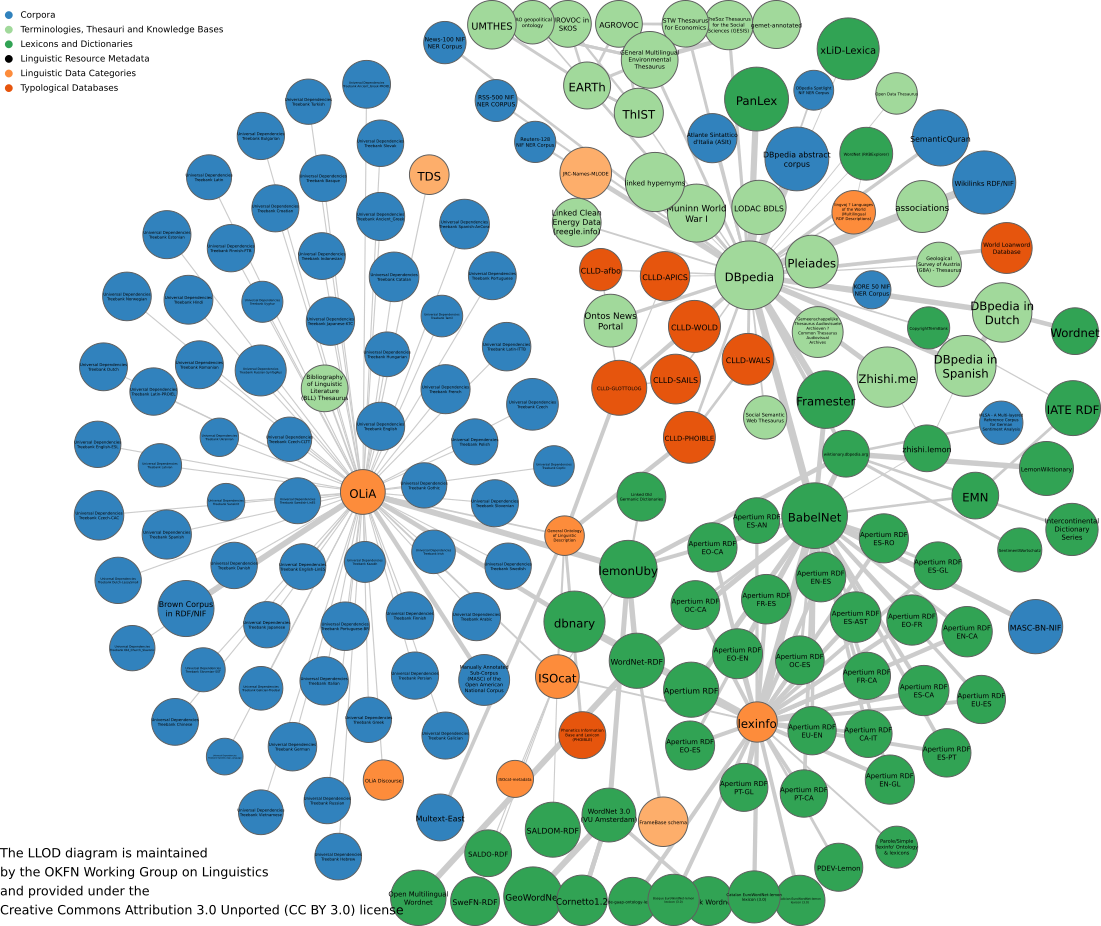
\includegraphics[width=1\textwidth]{img/llod.png}
 \caption{The Linguists Linked Open Data cloud \citep{chiarcos2012linking}}
 \label{fig:llod}
\end{figure}

Linghub \citep{mccrae2015linghub, mccrae2015reconciling} was created to allow for mining of all available databases - including META-SHARE, LRE Map, Datahub, and CLARIN's VLO - using SPARQL, a query language that works for Semantic Web ontologies encoded in RDF. Since publishing \citet{mccrae2015linghub}, OLAC has allowed its resources to also be mined.\footnote{\href{http://www.language-archives.org/news.html\#llod}{http://www.language-archives.org/news.html\#llod}. \last{April~26}} At this point, there are few large repositories of language resource data which are unable to be queried. However, linked data has the existential failing of only including metadata which has been included in the available data sources. It is a fantastic resource for finding corpora, and \citet{mccrae2015linghub} gives several examples of finding data through the cloud;  it is also an exceptional way to mine the LRE map database, which provides names of language resources for NLP tooling. But there is a barrier to entry of learning SPARQL and using an available portal, and any work outside of the curated, largely academic resources may not be available.

The linked open data cloud and Linghub also do not explicitly cater to LRLs, although there has been some work in this area \citep{huang2017linking}.

\subsection{Multilingual NLP libraries}
\label{subsec:popular-open-source-libraries}

While searching for code that has been tagged with metadata noting the language it serves has some merits, there are also possibilities for using generic code on many languages. For instance, \citet{bender2016linguistic} explores the field of multilingual NLP (now decades old; for instance, \citet{kay1997proper} called for this in the 90s), pointing out that there is a growing body of research that uses language typology to abstract and identify language features which allow for applying NLP systems from one language to another.

\begin{quote}
Businesses developing commercial products with NLP are interested in the markets represented by {\tt low resource languages} (LRLs; i.e., those languages for which there are not many digitized data sets or basic NLP systems such as part-of-speech taggers or morphological or syntactic parsers), some of which represent very large populations in emerging economies. Finally, researchers looking to apply NLP techniques to assist in endangered language documentation are naturally interested in developing NLP systems that work across very diverse languages.\citep[646]{bender2016linguistic}
\end{quote}

\citet{bender2016linguistic} goes on to mention the LinGo Matrix system \citep{bender2002grammar, drellishak2005coordination} that can be used to create rule-based grammars for natural languages using linguistic typographical data. The LinGo Matrix, and all work within the DELPH-IN system (a collaboration looking mainly at the Head-Driven Phrase Structure Grammar and Minimal Recursion Semantics) is open source.\footnote{\href{http://www.delph-in.net/wiki/index.php/Software}{http://www.delph-in.net/wiki/index.php/Software}. \last{April~26}}

They also mention projecting resources across languages, such as \citet{yarowsky2001inducing}, who projected linguistic annotations like POS tags and noun phrase parsing from English to French and Chinese, by using bilingual texts that had been word-aligned. This was extended in the previously mentioned \citet{agic2015if}, who similar POS tagger projection for one hundred LRLs. Their code is open source on Bitbucket.\footnote{\href{https://bitbucket.org/lowlands/}{https://bitbucket.org/lowlands/}. \last{April~26}}

This avenue of research is fascinating and broad, because it allows for small tools to be applied to other LRLs at a minimal cost. A study involving looking at all of the available research, with an in-depth look in each scientific article that includes links to source code, would be warranted and welcomed. It is unfortunately largely out of scope for this thesis; it is enough, here, to know that open source code for LRLs is dependent upon academics working in this field sharing their code on large repositories, and that this code must also be adapted to each particular LRL, which, while an extensive task, is made easier through multilingual NLP and cross-linguistic projection.

At a lower level, there are NLP toolkits which are useful for working with LRL datasets, which are language agnostic. The most well known is arguably the Natural Language Toolkit (NTLK)\footnote{\href{http://www.nltk.org/}{http://www.nltk.org/}. \last{April~26}} \citep{bird2006nltk}, a free and open source Python library that enables users to interface with over fifty different corpora and lexical resources, and which provides a suite of tools such as tokenizers and parsers which can be used in sparse data contexts. A primer written by the main creators \citep{bird2009natural}\footnote{Available online at \href{http://nltk.org/book}{http://nltk.org/book}. \last{April~26}}, is used frequently in natural language processing classes written by the creators. It is licensed under the Apache 2.0 license, an open source license \footnote{\href{https://github.com/nltk/nltk/blob/develop/LICENSE.txt}{https://github.com/nltk/nltk/blob/develop/LICENSE.txt}. \last{April~26}}. On GitHub, there are currently 204 contributors listed\footnote{\href{https://github.com/nltk/nltk/graphs/contributors}{https://github.com/nltk/nltk/graphs/contributors}. \last{April~10}}, and the contribution history in Git shows 234 (found by using the command {\tt git authors}). Some of the resources within NLTK work especially well with LRLs. For instance, in 2015, NLTK added machine translation libraries, including popular ones such as IBM Models 1-3 and BLEU.

By open sourcing their code, the NLTK authors have allowed it to be adapted and re-used. Currently, there are several ports, or reimplementations in another programming language which allows use in different coding language ecosystems. One of these is the JavaScript language implementation.\footnote{\href{https://github.com/NaturalNode/natural}{https://github.com/NaturalNode/natural}. \last{April~26}} This has 6700 stars on GitHub, which, since they reflect favouritism from individual users, is a good indicator of community vitality and use, and 88 contributors. The port is also open source, under an MIT license.\footnote{\href{https://github.com/NaturalNode/natural\#license}{https://github.com/NaturalNode/natural\#license}. \last{April~26}}

It is difficult to track usage of these open source software packages by LRL communities or researchers, as, once downloaded, there are no convenient metrics which lead back to the original source. Code, when run, generally leaves no trace. Again, the fundamental problem of tracking LRL open source software inhibits understanding the ecosystem, but it is clear from individual anecdotes and through scientific citations that work is being done in this area.

\subsection{A GitHub database for open source code}
\label{sec:solutions}

\begin{quote}
Currently, two approaches to metadata collection for language resources can be distinguished. Firstly, we distinguish a curatorial approach to metadata collection in which a repository of language resource metadata is maintained by a cross-institution organization ... This approach is characterized though high-quality metadata that are entered by experts, at the expense of coverage. A collaborative approach, on the other hand, allows anyone to publish language resource metadata. ... A process for controlling the quality of metadata entered is typically lacking for such collaborative repositories, leading to less qualitative metadata and inhomogeneous metadata resulting from free-text fields, user-provided tags and the lack of controlled vocabularies.
\end{quote}

\citet{mccrae2015linghub}, above, note that there are multiple ways of collecting metadata around resources, which provide their motivation to combine the two in Linghub. Here, I present a database built using a combination of the two; a curatorial, crowd-sourced database of language resources. This database has a mild advantage over Linghub and other large databases in that it is also decentralised, easily accessible and readable without learning a new language, and has a lower barrier to data entry.

Presented first in \citet{CCURL}, {\tt low-resource-languages} is a list of code resources for LRLs available on GitHub, available (under my namespace) at \href{https://github.com/RichardLitt/low-resource-languages}{https://github.com/RichardLitt/low-resource-languages}.\footnote{This was formerly called {\tt endangered-languages}. It was renamed to reflect attitudes mentioned in Section~\ref{subsubsec:response}.} The list is structured in Markdown\footnote{\href{https://daringfireball.net/projects/markdown/syntax}{https://daringfireball.net/projects/markdown/syntax}. \last{April~26}}, a lightweight format for text that is rendered natively on GitHub and is an industry standard in open source for structuring text documents.

Instead of using an XML or RDF representation that needs to be shown through a portal, this list natively works as a text list, as well, although the metadata is not as well structured and does not lend itself to aggregation in the same fashion. Making a scraper that would automatically translate the data into XML would be trivial. However, the benefit of using Markdown is that anyone on GitHub can easily parse and analyse the data directly, and that anyone can access and submit patches to add to the list. On GitHub, social coding conventions surrounding patches - called {\it pull requests} - allows for easy quality assurance of the data, as anyone suggesting an addition or deletion has to wait for a code maintainer to verify that their contribution is up to standard. This allows for a curated, collaborative approach to documentation and metadata aggregation. Curation occurs largely through my acceptance of related pull requests, along with other maintainers of the list - currently, Hugh Patterson of SIL\footnote{\href{https://github.com/HughP}{https://github.com/HughP}. \last{April~26}}, @cesine\footnote{\href{https://github.com/cesine}{https://github.com/cesine}. \last{April~26}} and @AnnaLuisaD of the Living Tongues Institute.\footnote{\href{https://github.com/AnnaLuisaD}{https://github.com/AnnaLuisaD}. \last{April~26}}

To date, there are 19 authors as recorded through {\tt git authors}, and 17 contributors recorded through GitHub's contributor view.\footnote{\href{https://github.com/RichardLitt/low-resource-languages/graphs/contributors}{https://github.com/RichardLitt/low-resource-languages/graphs/contributors}. \last{April~26}} Most pull requests came from @cesine, followed by @HughP. Six users contributed more than two pull requests. This data\footnote{\href{https://gist.github.com/RichardLitt/e60bcf9f399939b16181bf25ad6da8ba}{Available at https://gist.github.com/RichardLitt/e60bcf9f399939b16181bf25ad6da8ba}. \last{April~26}} came from an analysis of contributions using the GitHub API by using the {\tt name-your-contributors}\footnote{\href{https://github.com/mntnr/name-your-contributors/}{https://github.com/mntnr/name-your-contributors/}. \last{April~27}} tool, by running {\tt name-your-contributors -u RichardLitt -r low-resource-languages}.

A large majority of these files were last touched by me,\footnote{This figure was calculated by running {\tt git blame README.md | grep "Richard" | wc -l}.} as I have frequently reorganised and edited the list. In the past two weeks, GitHub's traffic shows 217 views by 37 unique visitors.\footnote{\href{https://github.com/RichardLitt/low-resource-languages/graphs/traffic}{https://github.com/RichardLitt/low-resource-languages/graphs/traffic}. \last{April~26}} There are a total of 39 forks, which reflects users who have copied the code to their own namespace (necessary for suggesting changes back to the main {\tt master} branch in GitHub). There are 166 stars and 24 watchers as of this writing.

There are 441 links available in the list,\footnote{This figure was calculated by running \texttt{grep "\textbackslash* \textbackslash[" README.md | wc -l}.} with hundreds of general resources and 32 different subsections available for specific low resource languages. Instead of tagging resources directly, they are placed in single sections that best describe the resource. The language specific sections are for: Albanian, Alutiiq, Amharic, Arabic, Bengali, Chichewa, Galician, Georgian, Guarani, Hausa, Hindi, H\o gnorsk, Inuktitut, Irish, Kinyarwanda, Lingala, Lushootseed, Malay, Malagasy, Manx, Migmaq, Minderico, Nishnaabe, Oromo, Quechua, Sami, Scottish Gaelic, Secwepemcts\'in, Somali, Tigrinya, Yiddish, and Zulu. Other sections cover: Single language lexicography projects and utilities, Utilities, Software, Keyboard Layout Configuration Helpers, Annotation, Format Specifications, i18n-related Repositories, Audio automation, Text-to-Speech
Text automation, Experimentation, Flashcards, Natural language generation, Computing systems, Android Applications, Chrome Extensions, FieldDB, FieldDB Webservices / Components / Plugins, Academic Research Paper Specific Repositories, Example Repositories, Language \& Code Interfaces, Fonts, Corpora, Organizations On GitHub, Other OSS Organizations, and Tutorials.

An example entry is provided below, for {\tt fast\_align} \citep{dyer2013simple}. The syntax of the example is as follows: A bullet point to place the item in a list; A link within brackets pointing to the GitHub repository where the open source code is stored, or to the resource elsewhere; and a basic description taken from the repository.

\begin{quote}
{\tt * [fast\_align](https://github.com/clab/fast\_align) - Simple, fast unsupervised word aligner.}
\end{quote}

In \citet{CCURL}, we described how the list is aimed at project managers, community developers doing language development, linguists, and software developers, mentioning some cases where developers reached out to say thank you for the list. To summarise our description: the list is for everyone, and the ease of accessibility of GitHub and rendered Markdown make it suitable for any audience. We did not then highlight how being on GitHub is of paramount importance. It is GitHub's social platform, and their extensive community, which makes this list most relevant. Since most open source code is on GitHub, then it follows that facilitating discovery by putting metadata directly on the site is useful step to undertake. As well, since the code is in an open source, Git repository, it is entirely possible for someone to easily copy the list and continue development and curation if for any reason my own copy goes down for any reason.

At LREC 2016 in Portoro\v{z}, where \citet{CCURL} was presented during the poster session\footnote{In reality, I presented it from my laptop as a way of facilitating input and discussion, as I felt that the analog quality of a poster would not properly convey the usefulness of the list, and as it was difficult to physically source a poster while hitchhiking from Italy.}, I collected responses on a Google Form from attendees (similar to data sourcing for LRE Maps, in some ways). There were 18 respondents. All but one of them said they have code related to endangered languages; only six of them had GitHub accounts (although one more had a Bitbucket account). Some of them have since contributed to the list.

There were at least two complaints; one of list quality, and another that the pages and subpages are often dead. The second concern has been fixed by implementing {\tt awesome\_bot}\footnote{\href{https://github.com/dkhamsing/awesome_bot}{https://github.com/dkhamsing/awesome\_bot}. \last{April~26}}, a tool which automatically checks all of the links and ensures that they resolve, and continuous integration tests with it through TravisCI.\footnote{\href{https://travis-ci.org/RichardLitt/low-resource-languages}{https://travis-ci.org/RichardLitt/low-resource-languages}. \last{April~26}} I have also cloned all of the Sourceforge repositories into GitHub repositories, to ensure that the open source licensed code is available in the GitHub ecosystem.

There is ongoing work to do curating the list, gathering sources, and improving the sections where data is stored. And, in the end, the magnitude of software resources is similar to what is found on any of the larger aggregators. It is unfortunately impossible to judge click-throughs and downloads of the list beyond what is provided above, given the nature of GitHub repositories and software. However, many tools mentioned in this list are not available on other providers - some novelty as an aggregator can be assumed. As \citet{CCURL} has no citations on Google Scholar as of yet, I assume that marketing work for the list is another future need to be met.

\subsection{Data and privacy}
\label{subsec:data-and-privacy}

Above, I have endeavoured to show that the state of open source work for LRLs is difficult to determine. Neither curated resources, linked aggregators of all resources, or mining the scientific literature are able to sufficiently answer the questions of how much code is out there, of what quality is that code, and where can language resource consumers best find their tools. However, it is probable that researchers working on a given language could easily find references to code which is relevant to their language, if it exists, using one of these three methodologies.

Unfortunately, a large amount of both data and tooling over that data is still not permissively licensed or available. Historically, linguists have not permissively licensed or provided open access to their corpora; it is specifically to combat this that large frameworks like the LDC or META-SHARE were created. However, these organisations do not solve some of the underlying issues regarding sharing data.

One issue which is unresolved is that of aligning incentives for researchers to open their research. Researching takes time and funding; opening up research to others can be seen as an act of na\"{i}ve altruism, especially in cases where the work could be easily used by competitive labs or businesses. For corpora to be open, providers may need to feel that they will be properly remunerated for the work. For some, this is less of a worry than citations and prestige. Citing linguistic data is not the same as citing research papers in journals or conferences, and only recently have there been movements towards citing data in itself. For instance, the Austin Principles for Data \citep{AustinPrinciples2017} were recently created to set guidelines for citing linguistic data. It emphasises that data is important and legitimate in the research cycle, that credit and attribution are needed where due, that it should be provided as evidence whenever there is a claim, that it should be referred to with DOIs that are persistent and unique, that it should be openly accessible, that it should be verifiable and specific to claims made, as well as interoperable and flexible in format. Each of these points could be expanded; for instance, evidentiality implies that in certain situations, producers should open confidential information if they wish to make a claim academically; for instance, Google researchers publishing results from their MT systems must also make their corpora available.

These principles can be extended to software, which historically is not cited academically (as in this paper, where a footnote to a website has for the most part sufficed). There is ongoing work in the sciences (if not in linguistics directly) on enforcing software citations \citep{DBLP:journals/corr/KatzCWHVHSJCCVL15, katz2016report}. The previously mentioned {\it Journal of Open Source Software} \citep{smith2018journal} is a good example of an effort to make code a citable object. To my knowledge, there has been no major effort linking linguistics corpora and the related tools under the same citable object. More research and collaboration here would be welcome.

Another facet regarding sharing data revolves around the sensitive nature of linguistic data itself, and ethical issues surrounding researchers or corpus architects. Participants who initially provide linguistic data may require permanent access to that data, and may wish to restrict access to others - for instance, in the case where stories or data are viewed as part of their cultural heritage, and which they view as private to their culture. Linguists taking data need to then document the wishes of the participants; and convey this on to data providers, to ensure that archivists respect the participants and the linguists wishes. Data which is gathered electronically {\it en masse} can  also lead to difficulties, as not all participants wishes can be easily taken into account (for instance, with large databases made by web crawlers). This milieu of needs and obligations can lead to licensing and access complications, especially with regard to LRLs. For instance, Chiarcos raised a question on the Open Linguistics mailing list\footnote{\href{https://lists.okfn.org/mailman/listinfo/open-linguistics}{https://lists.okfn.org/mailman/listinfo/open-linguistics}. \last{April~27}} regarding the legality of sharing Bible translations under EU and US law, and whether or not reuse of this data would constitute copyright violations for researchers who use the data.\footnote{\href{https://lists.okfn.org/pipermail/open-linguistics/2017-April/001359.html}{https://lists.okfn.org/pipermail/open-linguistics/2017-April/001359.html}. \last{April~27}} (There was no clear resolution in this case). There is a host of active research and discussion around this topic; \citet{liberman2000legal, newman2007copyright, rice2006ethical, austin2010communities, o2010ethical, cushman2013wampum} are recommended for further reading.

Sometimes, privacy revolves less around the users or the language communities, and more around researchers not wishing to open source their code until they are done developing their project, or until a grant ends, or until they are safe that they won't be scooped by other researchers. Other factors include the brevity of some academic funding cycles, concerns about scope, or lack of education regarding how open source works. However, the landscape is changing slowly. For instance, in a paper describing a tool for sharing interlinearised and lexical data in different formats, \citet[132]{kaufman2018kratylos} note that "Kratylos will be made open-source and accessible to the public through a GitHub repository at the end of the current grant period. Kratylos is built entirely from open- source software itself and transcodes proprietary media formats into the open-source codecs Ogg Vorbis (for audio) and Ogg Theora (for video)."\footnote{To date, this has not been open sourced. \href{http://elalliance.org/programs/documentation/kratylos/}{\nolinkurl{http://elalliance.org/programs/documentation/kratylos/}}. \last{April~27}} This is particularly insightful, as it shows that open source archives can arise out of initial closed-source development. Open source is not always a static state for code; and it is becoming more common to see open source code for LRL NLP as researchers become more familiar with current trends in software development.

% Removed as we cover this, basically, in Open Source
%\subsection{Data permanence and interoperability}

%\subsubsection{i18n documentation for larger open source tools}
%In some cases, tools themselves may canonically be used for NLP, but may also be translated into LRLs, thus allowing LRL developers to use the code themselves for bootstrapping their tools. For example, Node has an i18n and l10n committee that works to translate tools - and there is some interested in working with LRLs. % This may be a stretch.
%Another instance would be code which has been ported into rare languages % cite uspanteko work in java

% Open Source code for endangered languages
% \subsection{BLARK}
% \subsection{NLTK and other larger libraries}
% \subsection{Other resources}
% \subsection{solutions}
% A database for open source code
% Describe github.com/RichardLitt/endangered-languages
% !TEX root = thesis.tex
\section{Case Studies}
\label{sec:case-studies}

After having done a broad review of open source code for low resource languages above, here I dive deeper by looking for resources for two languages in particular: Scottish Gaelic and Naskapi. Both of these are living languages with speaking communities, although their size, coverage by academic research, and political situations are slightly different. Searching for resources for a specific language is most likely the most common use-case for users interested in LRLs, especially as the majority of LRL researchers work with a single language or a suite of languages that they use themselves, as opposed to researchers working on quantitative studies of languages in general. A deep dive should illuminate how open source methodologies can drive language development.

\subsection{Scottish Gaelic}
\label{sec:gaelic}

Scottish Gaelic (G\`aidhlig is the autonym) is a Celtic language spoken by roughly 60,000 people mainly in the United Kingdom and to a lesser extent in Canada. Gaelic - sometimes called Scots Gaelic, simply Gaelic, or the Gaelic - is a Goidelic or Q-Celtic language, along with Manx and Irish (also sometimes called Irish Gaelic, but here always referred to as Irish). This means that, while related to the Brythonic languages of Welsh, Cornish and Breton, it is different enough to not be able to benefit from the many resources available in Welsh, which, while endangered, has a much stronger academic interest and presence in the United Kingdom, with roughly half a million speakers. Gaelic has traditionally been heavily repressed, both politically and culturally, which has lead to its usage in largely restricted or rural areas, and in the domains of the house, church, and family \citep{mackinnon1991past}.

The 2011 Scottish Census indicates that out of the total amount of Gaelic speakers, only around half - 32,191 person to be exact - read and write in Gaelic.\footnote{\href{http://www.scotlandscensus.gov.uk/}{http://www.scotlandscensus.gov.uk/}. \last{April~27}} 6,218 speak and read the language, but do not write it, while 4,646 can read it, but do not speak or write it. Gaelic officially is not a national language, although it is afforded certain protections under the European Charter for Regional or Minority Languages\footnote{\href{https://www.coe.int/en/web/conventions/full-list/-/conventions/treaty/148}{https://www.coe.int/en/web/conventions/full-list/-/conventions/treaty/148}. \last{April~27}} (although, as this is an EU charter, it is unclear whether Britain will continue to ratify it following their impending exit from the European Union). The Gaelic Language (Scotland) Act of 2005 (GLS) gave Gaelic official status as an official language of Scotland,\footnote{\href{http://www.legislation.gov.uk/asp/2005/7}{http://www.legislation.gov.uk/asp/2005/7}. \last{April~27}} and set up the B\`ord na G\`aidhlig\footnote{\href{http://www.gaidhlig.scot/}{http://www.gaidhlig.scot/}. \last{April~27}} as a language developmental body tasked with protecting and vitalising the Gaelic language.

The B\`ord officially is tasked with promoting and facilitating educational materials, but the initial charter makes no mention of language technology. The National Gaelic Language Plan 2018-2023\footnote{\href{http://www.gaidhlig.scot/launch-of-the-new-national-gaelic-language-plan/}{http://www.gaidhlig.scot/launch-of-the-new-national-gaelic-language-plan/}. \last{April~27}} \citep{bord2018national} mention the Digital Archive of Scottish Gaelic (DASG),\footnote{\href{http://dasg.ac.uk/en}{http://dasg.ac.uk/en}. \last{April~27}} the largest corpus project for Gaelic, but do not specify other language technology being developed (excepting a brief mention of working with Ireland and Nova Scotia developing shared technology and resources). There are some primary and secondary schools, as well as various Gaelic Language and Studies degrees at English-speaking universities, as well as one Gaelic-speaking university Sabhal M\`or Ostaig\footnote{\href{http://www.smo.uhi.ac.uk/en/}{http://www.smo.uhi.ac.uk/en/}. \last{April~27}} on Skye; educational material from the B\`ord is mainly focused in these areas.

\subsubsection{Language vitality status}
\label{sec:gaelic-vitality-status}

Gaelic has an EGIDS rating of 2, as it is a provincial language given the 2005 GLS Act.\footnote{\href{https://www.ethnologue.com/language/gla}{https://www.ethnologue.com/language/gla}. \last{April~27}}  \citet{lewis2009ethnologue} note regarding language use that "Resurgence of interest in Scottish Gaelic in 1990s. A number of children learn the language but there are serious problems in language maintenance even in the core areas \citep{salminen2007endangered}. Home, church, community." UNESCO judges it to be {\it definitely endangered}.\footnote{\href{http://www.unesco.org/languages-atlas/en/atlasmap/language-iso-gla.html}{http://www.unesco.org/languages-atlas/en/atlasmap/language-iso-gla.html}. \last{April~27}} The Endangered Languages Project describes it as Threatened or Vulnerable, depending on the source,\footnote{\href{http://endangeredlanguages.com/lang/3049}{http://endangeredlanguages.com/lang/3049}. \last{April~27}} as \citet{salminen2007europe} gives a much smaller population number of 20k for speakers than the other census-based data. \citepos{kornai2013digital} rating declares it as {\it Living}.\footnote{\href{https://hlt.bme.hu/en/dld/language/4656}{https://hlt.bme.hu/en/dld/language/4656}. \last{April~27}} These ratings are summarized in Table~\ref{table:gaelic}.

\begin{table}
\centering
\begin{tabular}{|p{5cm}|p{5cm}|} \hline
{\bf Scale} & {\bf Grade} \\ \hline
UNESCO & Definitely endangered\\ \hline
Ethnologue (EGIDS) & 2 (Provincial) \\ \hline
LEI & Threatened or Vulnerable \\ \hline
Kornai & Living \\ \hline
\end{tabular}
\caption{Scale for Gaelic}
\label{table:gaelic}
\end{table}

\subsubsection{Language resources}
\label{subsec:gaelic-resources}

Gaelic has a long, written history. Today, there are a plethora of written, audio, and video resources. Some of these have been bundled into linguistic corpora. The DASG is the largest corpus for Gaelic available on the web; however, it is not permissively licensed for modification, distribution, or reproduction, and so cannot be considered open source (although it is open access).\footnote{\href{http://dasg.ac.uk/about/terms/en}{http://dasg.ac.uk/about/terms/en}. \last{April~27}} OLAC has 26 resources for Gaelic, including large multilingual corpora, as well.\footnote{\href{http://www.language-archives.org/language/gla}{http://www.language-archives.org/language/gla}. \last{April~27}} A large corpus compiled by An Crub\'ad\'an is available online \footnote{\href{http://crubadan.org/languages/gd}{http://crubadan.org/languages/gd}. \last{April~27}} \citep{scannell2007crubadan}. WALS has 61 typological features listed for Gaelic,\footnote{\href{http://wals.info/languoid/lect/wals_code_gae}{http://wals.info/languoid/lect/wals\_code\_gae}. \last{April~27}} and Glottolog 35 references.\footnote{\href{http://glottolog.org/resource/languoid/id/scot1245}{http://glottolog.org/resource/languoid/id/scot1245}. \last{April~27}} ODIN has 59 IGT entries for Scottish Gaelic.\footnote{\href{http://odin.linguistlist.org/}{http://odin.linguistlist.org/}. \last{April~27}}

Some of these corpora are annotated - for instance, the Annotated Reference Corpus of Scottish Gaelic (ARCOSG)\footnote{\href{https://datashare.is.ed.ac.uk/handle/10283/2011}{https://datashare.is.ed.ac.uk/handle/10283/2011}. \last{April~27}} \citep{ARCOSG2016, lamb2014scottish}, which used an Irish POS tagger \citep{ui2006part} to project annotations, and which was funded by the B\`ord na G\`aighlig. This resource was used to automatically derive categorial grammars \citep{batchelor2016automatic}, and to develop POS taggers directly for Gaelic \citep{lamb2014developing}. A dependency-structure corpus is being developed \citep{batchelor2014gdbank}, as are word-embedding models \citep{lamb2016developing}. The source code for \citet{batchelor2014gdbank, batchelor2016automatic} is available on GitHub.\footnote{\href{https://github.com/colinbatchelor/gdbank/}{https://github.com/colinbatchelor/gdbank/}. \last{April~27}} Some of these papers were presented at the first Celtic Language Technology Workshop in Dublin in 2014. The amount of resources show clearly that Gaelic is not entirely on the fringe of academic research, although it is generally considered a low resource language.

\citet{scannell2007crubadan} and contributors\footnote{\href{http://crubadan.org/acknowldegments}{http://crubadan.org/acknowldegments}. \last{May~2}} used the Cr\'ubad\'an corpus to create an open source Hunspell spellchecker,\footnote{\href{https://github.com/kscanne/hunspell-gd}{https://github.com/kscanne/hunspell-gd}. \last{April~27}} which is the spellchecker for "LibreOffice, OpenOffice.org, Mozilla Firefox 3 and Thunderbird, Google Chrome, and it is also used by proprietary software packages, like macOS, InDesign, memoQ, Opera and SDL Trados."\footnote{\href{https://hunspell.github.io/}{https://hunspell.github.io/}. \last{April~27}} This spellchecker was built with the help of Michael Bauer, an independent Gaelic technologist who runs a small Gaelic technology consultancy called Am Faclair Beag,\footnote{\href{http://www.faclair.com/}{http://www.faclair.com/}. \last{April~27}} and also has ports for OpenOffice directly\footnote{\href{https://addons.mozilla.org/ga-IE/firefox/addon/scottish-gaelic-spell-checker/}{https://addons.mozilla.org/ga-IE/firefox/addon/scottish-gaelic-spell-checker/}. \last{April~27}} and a Firefox extension.\footnote{\href{https://extensions.openoffice.org/en/project/faclair-afb}{https://extensions.openoffice.org/en/project/faclair-afb}. \last{April~27}} An Faclair Beag also offers an online dictionary with over 85k words\footnote{\href{http://www.faclair.com/GaelicDictionaryAbout.html\#About}{http://www.faclair.com/GaelicDictionaryAbout.html\#About}. \last{April~27}}
 (and almost a million forms\footnote{\href{http://www.faclair.com/News.html}{http://www.faclair.com/News.html}. \last{April~27}}) and in inbuilt lemmatizer.\footnote{\href{http://www.faclair.com/News.html}{http://www.faclair.com/News.html}. \last{April~27}} Another spellchecker also exists on GitHub,\footnote{\href{https://github.com/gooselinux/hunspell-gd}{https://github.com/gooselinux/hunspell-gd}. \last{April~27}} but it is probably derivative, and it has not been worked on recently.

 More complicated, higher level technology also exists. Previous academic work on Gaelic text-to-speech systems (TTS) stretches back at least 20 years; a diphone text-to-speech system for Gaelic was developed, for instance, in 1997, by \citet{wolters1997diphone}, although that is not open source. Today, there is a proprietary synthetic TTS system called Ceitidh\footnote{\href{https://www.cereproc.com/en/CereProc_Gaelic_Synthetic_Voice_Ceitidh}{https://www.cereproc.com/en/CereProc\_Gaelic\_Synthetic\_Voice\_Ceitidh}. \last{April~27}} (pronounced `Katie'), created by a private Gaelic company together with funding from the Scottish Government and the B\`ord na G\`aidghlig. Although Ceitidh is available to developers and students at a reduced or free fee, it is not entirely open source. There are almost no open source sound resources. The main reason is that there is no overall quality assurance for Gaelic sound uploaded online. For large languages, this is not a problem; however, for smaller languages, the size of the corpus means that much of the content may come from only a few sources, none of which may be ideal. This issue may involve general lack of relevance of sound files, or poor quality recordings, or any dialect or non-mainstream features slipping in. Ceitidh was based on original audio files from Kirsteen MacDonald (in Gaelic, Kirsteen NicDh\`{o}mhnaill), some of whose content (while not vetted by an independent linguist) are available on LearnGaelic.scot,\footnote{\href{https://learngaelic.scot/}{https://learngaelic.scot/}. \last{April~27}} which could be hypothetically used to build an open source TTS system. However, quality assurance would be an arduous step.

Navigating resources to identify what is open source and what is not is difficult. As mentioned in Section~\ref{subsec:where-is-open-source-code}, one of the OSI's definitions for open source was that it be well publicised. This cannot be said to be the case for coding resources for Gaelic; there is no central location for viewing tools. The LRE Map has no Gaelic resources, although a POS Tagger, two corpora, a tokenizer, and Babouk corpus tool resource are mentioned for Irish.\footnote{\href{http://www.resourcebook.eu/searchll.php}{http://www.resourcebook.eu/searchll.php}. \last{April~27}} Linghub returns 30 entries - not many, considering it is an aggregator.\footnote{\href{http://linghub.org/search/?query=Gaelic}{http://linghub.org/search/?query=Gaelic}. \last{April~27}} GitHub returns 62 repositories that mention Gaelic,\footnote{\href{https://github.com/search?q=gaelic}{https://github.com/search?q=gaelic}. \last{April~27}} although it is unclear if these are for Irish.

The best resource is arguably Kornai's lab page\footnote{\href{https://hlt.bme.hu/en/dld/language/4656}{https://hlt.bme.hu/en/dld/language/4656}. \last{April~27}} (again, in development). While not linking directly, it does give some information. It notes that there are: several language packs at the OS level for Ubuntu and Windows input, but not one for Mac, probably because Gaelic uses the Roman alphabet and a UK keyboard suffices for most needs;\footnote{I use the US International Keyboard with OSX to type Gaelic accents, myself, and have never needed another keyboard layout for this} a large Wikipedia; a Hunspell checker; OLAC texts (with marginally out of date numbers); a large Cr\'ubad\'an corpus (1,541,302 words and 17,308 documents), as well as a large Indigenous Tweets corpus with half a million words; and general coverage in Omniglot,\footnote{\href{http://omniglot.com/writing/gaelic.htm}{http://omniglot.com/writing/gaelic.htm}. \last{April~27}} bible.org,\footnote{\href{https://bible.org/}{https://bible.org/}. \last{April~27}} Panlex,\footnote{\href{https://panlex.org/}{https://panlex.org/}. \last{April~27}} and the Leipzig corpora \citep{goldhahn2012building}.\footnote{\href{http://wortschatz.uni-leipzig.de/en/download/}{http://wortschatz.uni-leipzig.de/en/download/}. \last{April~27}} Some of the stats are dubious. For instance, 15k wikipedia users seems odd for a language where there a total population of 30k literate speakers; and it is in WALS, quite clearly. However, in general, this gives a better overview than any other source.

As far as I am aware, the highest amount of code resources for Gaelic which are directly linked and open source is the corpus described in Section~\ref{sec:solutions}. There are six resources mentioned in the list,\footnote{\href{https://github.com/RichardLitt/low-resource-languages\#scottish-gaelic}{https://github.com/RichardLitt/low-resource-languages\#scottish-gaelic}. \last{April~27}} which was largely sourced by manually inspecting each of the GitHub repositories mentioning "Gaelic", and also through personal curation during general research for this paper.

Ideally, researchers would start to open source more of their code involving Gaelic. However, there are so few researchers and language communities currently working on Gaelic HLT that this may be a na\"{i}ve wish. Indeed, the main researcher over the past decade for Gaelic releases most of his code publicly - that is, Kevin Scannell of \citet{scannell2007crubadan}. And his focus is mainly on Irish. One solution would be to implement a Scottish Gaelic computational linguistics course at one of the major Scottish universities, such as the University of Edinburgh, Glasgow, St. Andrews, or potentially at Sabhal M\`or Ostaig. This option would reward further lines of inquiry.

% TODO Mention Scannell's pooling paper
% TODO Mention Salt on a shoestring

\subsection{Naskapi}
\label{sec:naskapi}

In October 2017 I travelled to Kawawachikamach and informally interviewed linguists working on a Naskapi Bible, visited the school and talked to teachers at length about language efforts there, and talked to individual Naskapi speakers about their thoughts on the language and how it is used. Below, I give a brief overview of Naskapi, note how it would be rated according the metrics covered in Section~\ref{subsec:metrics}, and discuss language resource development. \citet{jancewicz2002applied} is the main source of published information on Naskapi computational developments; I give an update, 15 years on, given my experience in Kawawachikamach. %I was unfortunately unable to meet Bill Jancewicz, the SIL missionary there, at that time.

\subsubsection{Language background}
\label{sec:naskapi-language-background}

Naskapi (autonymically \sylla{naskapi} naskapi or \sylla{iyuw iyimuun} iyuw iyimuun) is a Cree language in the Algonquin family spoken in central Quebec \citep{MacKenzie-and-Jancewicz-1994}. Virtually the entire population of around 900 Naskapi live within the reservation Kawawachikamach, around 10 miles from Schefferville, QC. There is another Naskapi community on the Labrador coast, who speak another dialect known as Mushuau Innu, which is out of scope of this paper. Schefferville is only accessible by train or plane, and contains another local tribe called the Innu (which has more than 17,000 members, scattered among Quebec and Labrador\footnote{\href{https://en.wikipedia.org/wiki/Innu}{https://en.wikipedia.org/wiki/Innu}. \last{April~27}}), who live on their own reservation and who speak Montagnais or Innu-aimun, a related language. The two languages are similar, and the Naskapi youth are often diglossic in Montagnais (but the Innu are often not) \citep{macKenzie1980towards}.

The Naskapi speak English as a first or second language, while the Innu speak French (and some speak three or all four languages). They moved to Kawawachikamach in the 1960s, after initially being resettled in Schefferville in the early 1950s. Some of the elders still remember being a nomadic people who followed caribou and were raised in the bush. However, half of the population is under the age of 16, and nationally the First Nations population is the largest growing population in Canada.\footnote{\href{http://www12.statcan.gc.ca/census-recensement/2016/dp-pd/index-eng.cfm}{http://www12.statcan.gc.ca/census-recensement/2016/dp-pd/index-eng.cfm}. \last{May~2}}

All of the Naskapi speak their own language regularly, in all contexts - excepting, perhaps, digitally. In the schools, there are Naskapi-only classes held until Grade 8 \citep{llewellyn2017oral}. While there are a few social workers, teachers, and nurses who speak solely English, most jobs in Kawawachikamach are held by Naskapi. There has been a long tradition of missionaries, and almost all of the Naskapi are Protestant. At church, they use Montagnais hymnals and a Montagnais bible.

\subsubsection{Language vitality status}
\label{sec:naskapi-vitality-status}

\citet{lewis2009ethnologue} classifies Naskapi as Level 4 (educational), and notes that "Literacy rate in L1: Western Naskapi: 50\%. Literacy rate in L2: 50\%. Ongoing community language program in Western Naskapi. All children through [sic] in kindergarten through grade 6 can read and write in the language (2017 N. Jancewicz).\footnote{This was gathered through personal communication with Norma Jean Jancewicz, one of the SIL missionary married couples together with Bill Jancewicz (SIL personal communication, 2018).} Taught in primary schools in Western Naskapi. Dictionary. Grammar. NT: 2007. "\footnote{\href{https://www.ethnologue.com/language/nsk}{https://www.ethnologue.com/language/nsk}. \last{April~27}} UNESCO defines it as {\it vulnerable}.\footnote{\href{http://www.unesco.org/languages-atlas/en/atlasmap/language-id-2354.html}{http://www.unesco.org/languages-atlas/en/atlasmap/language-id-2354.html}. \last{April~27}} \citepos{kornai2013digital} digital vitality index awkwardly declares it to be {\it dead}.\footnote{\href{https://hlt.bme.hu/en/dld/language/5651}{https://hlt.bme.hu/en/dld/language/5651}. \last{April~27}} Naskapi does not appear at all on the Endangered Languages Project. These ratings are displayed in Table~\ref{table:naskapi}.

\begin{table}
\centering
\begin{tabular}{|p{5cm}|p{5cm}|} \hline
{\bf Scale} & {\bf Grade} \\ \hline
UNESCO & Vulnerable \\ \hline
Ethnologue (EGIDS) & 4 (Educational) \\ \hline
LEI & -- \\ \hline
Kornai & Dead \\ \hline
\end{tabular}
\caption{Scale for Naskapi}
\label{table:naskapi}
\end{table}

The {\it dead} terminology used to describe Naskapi by \citepos{kornai2013digital} metric reflects the metric being only applied to online corpora (which is minimal), and, regardless of the insensitivity of the nomenclature, it does have some merit here. When looking at the resources listed, there are no language packs for software, no Wikipedia articles, no Hunspell, no primary texts listed in OLAC, only 2415 words listed in the Cr\'ubad\'an corpus, no Indigenous tweets, no Swadesh lists, and only a brief mention in Panlex translations (90 words), and in Omniglot. Once again the data may not be perfect - this source lists the EGIDS rating at Level 5 (which I would disagree with, placing it in back in Level 4, as "The language is in vigorous use, with standardisation and literature being sustained through a widespread system of institutionally supported education.")

ODIN has exactly one IGT entry for Naskapi, from \citet{richards2004syntax}. This means that noting the translation in Example~\ref{igt1} may may double the size of ODIN's entries, although it is not the first entry in the literature (this lexeme is mentioned in \citet{macKenzie1980towards}).\footnote{This might also be transliterated as `wabush`, although it would not match the Naskapi phonological inventory. Wabush is the name of a town in Labrador, which I was told meant `hare' or `rabbit', and my pronunciation was not corrected.}

\begin{exe}
\ex
\gll wa:pus\\
hare\\
\trans `hare'
\label{igt1}
\end{exe}

Regardless of this paucity of data, there are certainly literary resources in Naskapi (see the next section) - if not many digitally. In the case of Naskapi, the Emergent level proposed by \citet{gibson2016assessing} may be more fitting than either Dead or Vital.

\subsubsection{Orthography}
Naskapi has two scripts; Latin and the Unified Canadian Aboriginal Syllabics \citep{wals-141}, which were added to Unicode in 1999.\footnote{\href{https://www.unicode.org/standard/supported.html}{https://www.unicode.org/standard/supported.html}. \last{April~27}} The Syllabics were introduced by missionaries in the 19th century, and quickly adopted by all Cree language communities, who approached near universal literacy \citep{bennett1991cree}. In Kawawachikamach and Schefferville (and on the train there), there are many examples of writing in syllabics. As well, Naskapi has its own standard orthographical conventions for Roman characters. For instance, a macron, such as \^u is used in place of a double \emph{uu} to indicate vowel length.

\citet{jancewicz2002applied} gives an insightful overview of computational technology in Naskapi. They note that Naskapi often were not involved in typesetting literature in syllabics, and that few became typists when the first syllabic typewriters were introduced. Jancewicz is particularly well placed as the author of this paper, as he and his wife were the first two missionaries sent from SIL to the Naskapi community (MacKenzie is also, as she has worked for decades with Cree communities as well as with the Naskapi). They worked with the Band Office (the local council) installing the first word processing system for syllabics, trained Naskapi speakers, and created the first Naskapi TrueType font.

Jancewicz also helped to install Keyman,\footnote{\href{https://keyman.com/}{https://keyman.com/}. \last{April~27}} "a keyboarding utility ... that allowed the programming of custom keyboard input for various languages and character sets." \citep[85]{jancewicz2002applied} Keyman is now free, open source software available on GitHub.\footnote{\href{https://github.com/keymanapp}{https://github.com/keymanapp}. \last{April~27}} It allows a user to type Roman letters which are converted to the right phrase in Syllabics, and is forgiving for phonemic variants. For instance, "ju", "chu", "tchu" and so on might all be interpreted and replaced by the appropriate syllabic \sylla{co}. % TODO Ask if this is the right syllabic
Keyman must be installed manually on each computer to use it, which reflects a considerable amount of upfront time for Jancewicz. Indeed, the importance of their support to Naskapi digital ascendancy cannot be understated (except, perhaps, by Jancewicz himself):

\begin{quote}
"Since 1988, the resident linguist has maintained all of his own language learning materials and language data on computer. He has also provided the local technical support that is needed in a small, isolated community, especially with regard to the esoteric development of computer programs that allow syllabic word processing. While it is not impossible to use computers in Native language work without a full-time, on-site computer resource person, it has been an obvious asset to have such a person available to provide training and technical support." \citep[86]{jancewicz2002applied}
\end{quote}

Currently, the school has a computer lab with over a dozen computers, but no in-house computer technician. One of the Wycliffe translators needed to visit the school to check on Keyman updates, and the students are not regularly trained in how to set up Keyman on their own, or how to set it up on their phones or other portable devices, although there have been efforts to train key teachers in how to teach computational use of Naskapi \citep{jancewicz1998developing}. While Facebook and other online platforms are increasingly popular, the majority of talking takes place in Naskapi written in local characters, or in English.

However, it is crucial that development and education regarding computational literacy continue to be mandated and improved. "Using a computer for mother-tongue language work raises speakers' assessment of the worth of their own language, as well as provides an avenue for sharing their work and ideas through reproduction and publication." \citet{jancewicz2002applied}

\citet{jancewicz2002applied} was written before wide adoption of the Unicode standard by browsers, and before the now omnipresent ubiquity of the internet and smartphones. \citet{jancewicz2012cree} gives an update on fonts available for Cree languages, including Naskapi. It also mentions Languagegeek,\footnote{\href{http://www.languagegeek.com/algon/naskapi/naskapi.html}{http://www.languagegeek.com/algon/naskapi/naskapi.html}. \last{May~3}} a website that has useful information on downloading fonts for Naskapi.

\begin{quote}
One of the most important sources for Cree Unicode fonts is the LanguageGeek website by Chris Harvey. Chris Harvey developed "Aboriginal Serif Unicode", which has gone through some changes and improvements. His current strategy is to serve logical regions of syllabic users with fonts that contain subsets of the UCAS block, rather than one font that contains them all. His work is very impressive and professional but some readers may find it difficult to read because of somewhat close letter- and especially word-spacing. \citep[17]{jancewicz2012cree}
\end{quote}

\subsubsection{Corpora creation}

In recent years, the Naskapi Development Council (NDC), which works with translators provided by the Band, has produced a Naskapi to English bilingual dictionary in three volumes \citep{MacKenzie-and-Jancewicz-1994}. The NDC is largely staffed by linguists from the Summer Institute of Linguistics, funded by Wycliffe Bible Translators and private fundraising from Christian communities.\footnote{\href{https://www.wycliffe.org/}{https://www.wycliffe.org/}. \last{April~27}} Today, the SIL linguists are a team of six: two long term linguists, and two pairs of husband and wife pairs who are training how to work as Bible translators in this community before moving on to working with other Cree communities in Canada. 

Naskapi does not have a complete Bible. A new testament, started in the 1970's, was recently published \citep{naskapi-new-testament}. Genesis, Exodus, and Psalms, have also been translated, and several children stories and books of oral legends from an elder have been produced - as well, \citet{jancewicz2002applied} note the creation of a monthly newsletter, a history, and translations of official business of the administrations (which may provide excellent multilingual corpora). The full-time translators are two people: a young woman in her mid-twenties, and an older man of around fifty years of age. At times, elders also contribute to the Bible translation effort by marking up pre-publication drafts, which they then go over with the translators.

When there is a need to come up with a new term, the elders are consulted, and they agree on an appropriate translation. For instance, {\it grill} is translated as `metal-net'. `grill' is not a  pre\"{e}xisting word in Naskapi, but `net' is, and it is easy to imagine the metaphor of a grill on which you braise meat as being a metal net. However, these decisions are not often used outside of the Bible. Likewise, when there is a term which needs to be invented at the school, the teachers there decide on an appropriate term - for instance, for situations like Halloween, where `Frankenstein' may need to be translated into a local alternative. These decisions are largely one-off, although they may be used year to year, and informally recorded in their respective domains.

The linguists use the Fieldworks Language Explorer (FLEx) \footnote{\href{https://software.sil.org/fieldworks/}{https://software.sil.org/fieldworks/}. \last{April~27}} to document new linguistic terms. FLEx was developed by SIL International, and provides linguists with an out-of-the-box solution for recording linguistics terms using interlinear glossed text. It is also open source, and available on GitHub.\footnote{\href{https://github.com/sillsdev/FieldWorks}{https://github.com/sillsdev/FieldWorks}. \last{April~27}} Users can export as a PDF (among other file formats), or export words to an online interface known as Webonary.\footnote{\href{https://www.webonary.org/configuring-the-dictionary-in-flex/}{https://www.webonary.org/configuring-the-dictionary-in-flex/}. \last{April~27}} This allows language workers to automatically create a useable, free dictionary for members of the community.

% TODO Ask if I can access the Webonary

\subsubsection{Computational tools}

There are no spell checkers, word lists, or large corpora available digitally except for the dictionary. As well as the SIL-sponsored Webonary, there is also work done by \href{http://atlas-ling.ca/}{\nolinkurl{http://atlas-ling.ca}}, which is a Canadian government-backed venture, originally cofounded by MacKenzie, who also worked on the Naskapi dictionary.\footnote{\href{http://atlas-ling.ca/}{http://atlas-ling.ca/}. \last{April~27}} This website has some options for looking at languages, but does not seem to be updated by local translators from the community. It is sourced from the previously published dictionary, which the SIL linguists have indicated is not up to date and has insufficient English to Naskapi translations. These are insufficient because of the nature of Naskapi; a root word is used with a slot system, and any word which mentions water is included under the English heading. This makes translating something as simple as "the mug is red" difficult, as one needs to know to look for `red' as a root word, and then to find the appropriate example from which you can extrapolate the correct form for translation.

There is a potentially large corpus of spoken language in Naskapi from the local radio station, but this has not been collected into a corpus. There does not appear to be any adult-level secular written corpora which could be utilised to jump-start a written corpus; \citet{jancewicz2002applied} points out that "While in some language communities it may be supposed that such an emphasis on the production of religious texts may limit the use of Native language literacy in secular community institutions, the Cree and Naskapi cultures treated in these case studies traditionally do not draw a sharp distinction between the secular and spiritual in their day-to-day life." It is also worth noting that the Band Office employs translators (who generally have other jobs - one this author talked to was a band Councilman, one of four elected officials underneath the Chief) who may be able to provide bilingual texts in English, French, or Innu.

All told, computational work that is easily accessible on the web is exceedingly limited. There are some websites in Naskapi, which could be used to make a small corpus, but there are no currently active projects working on collecting corpora for the purpose of linguistic study, and neither is there an active academic community working on Naskapi outside of the SIL translators, who may occasionally publish a paper (or, of course, a dictionary or physical book).

While FLEx is open source, none of the linguists edit the code for it or use the codebase, depending on SIL International to keep the product up to date. Keyman is likewise not edited, although it is installed on local computers. The Naskapi community website, run by the Naskapi Nation of Kawawachikamach, does have a webpage on installing syllabics,\footnote{\href{http://www.naskapi.ca/en/Install-syllabics}{http://www.naskapi.ca/en/Install-syllabics}. \last{April~27}} which may be useful for some speakers.

\subsubsection{Naskapi language resource status today}

Today, a small group of external linguists still provide much of the language resources for the community, although collaboration with the Band continues.

\begin{quote}
"The authors hope that the dichotomy between "resource people" and "aboriginal people" reflected in the section headings above would become less and less distinct. ... As a growing number of local people gain experience and expertise to become their own resource persons, such a dichotomy will dissolve, and all the vital resources for language development will exist at a community level. However, until this ideal is realised, small language communities such as these must continue to identify and avail themselves of professional and academic resources found outside their communities." \citep[89]{jancewicz2002applied}
\end{quote}

This remains just as true, fifteen years on. There is work which could be done; for instance, moving the silo'ed dictionary efforts into the public web, and using bilingual texts from the Band Office to bootstrap corpora, POS taggers, spellcheckers (there is not a Hunspell yet), and perhaps MT systems. However, this work would need to be matched by on-the-ground work by local community members - and, as \citet[90]{jancewicz2002applied} finally notes: "The initial learning curve is sometimes steep, but there is no substitute for hands-on experience."

Open source is less of a concern for Naskapi as is general software; the community is so small that any code is liable to made by community members and open sourced, anyway. However, the tools which the linguists use to develop languages benefit from open source. Any SIL missionary can contribute to FLEx, which means that incremental changes in different communities can be folded back into work in Naskapi. Likewise, any work done on Cree or any related languages can be applied or projected onto Naskapi more easily if it is open source. Open source is not a {\it sine qua non} for Naskapi technological development, then; but it could be a benefit.

% TODO Ask Bill for a copy of his MA thesis "Grammar enhanced biliteracy: Naskapi language structures for facilitating reading in Naskapi"

% \subsection{Gaelic}
% \subsection{Naskapi}
% \subsection{Kilangi} Another possible usecase?
% !TEX root = thesis.tex
\section{Methods}
\label{sec:methods}

It is customary when doing a quantitative review to give advice around best practices, to make not just the next researcher's job easier, but also to help life the quality of the state of the field, in general. In my research, I have often done the same: \citet{DBLP:journals/corr/KatzCWHVHSJCCVL15}, which came out of a workshop on sustainable software in the sciences, does a reasonable job of doing this for software citation; \citet{LittIDCC} for scientific workflows; \citet{LittEdulearn} for crowdsourcing learning materials by students in the classroom; and \citet{wiggins2013data} for public participation in science. Here, in the same vein, are some recommendations for utilising open source for LRL NLP.

\subsection{Choosing a license}
\label{choosing-a-license}

Legal advice on the internet is often preceded by the initialism IANAL, stating "I am not a lawyer", or sometimes "I am not your lawyer." The following is not meant to constitute legal advice, and I am not liable for any advice given here.

That having been said, licensing software in the open domain is definitely to been encouraged. Section~\ref{subsec:licenses} lists many licenses which are considered open source; any of them should work for most purposes (although I would recommend against the Unlicense in favour of a CC0 license, following the Free Software Foundation's advice that it is "more thorough and mature".\footnote{\href{https://www.gnu.org/licenses/license-list.html\#Unlicense}{https://www.gnu.org/licenses/license-list.html\#Unlicense}. \last{May~3}})

\citet{streiter2006implementing} recommends using the GPL license for any software contributed into a software pool, their terminology for community-curated open source software. They also recommend the lesser GPL, as needed; however, GPL is preferred because it enforces that all modifications to software be brought back to the original moderator for acknowledgement, which allows for the source code to be updated. A specific example they give is of Scannell's Irish spell checker.

\begin{quote}
The case of Irish language spell checking is illustrative in this regard. Kevin Scannell developed an Irish spell checker and morphology engine in 2000, integrated it into the Ispell pool, and released everything under the GPL. Independent work at Microsoft Ireland and Trinity College Dublin led to a Microsoft-licensed Irish spell checker in 2002, but with no source code or word lists made freely available. Now, roughly five years later, the GPL tool has been updated a dozen times thanks to contributions from the community, and the data have been used directly in several advanced NLP tools, including a grammar checker and an MT system. The closed-source word list has not, to our knowledge, been updated at all since its initial release. Indeed, a version of the free word list, repackaged for use with Microsoft Word, has all but supplanted use of the Microsoft-licensed tool in the Irish-speaking community. \citep[282-283]{streiter2006implementing}
\end{quote}

I would recommend against GPL for another reason; code is often maintained by a single author, and GPL puts undo pressure on the author to maintain the code in the long term. Maintenance of code is difficult, as it involves work time that is often not paid, and as it requires that the author of the code sets expectations around levels of maintenance.

For this reason, I have always licensed my own code under the MIT license, which waives all liability and insists that the code therein is provided as-is. This makes long term maintenance easier on the maintainers, as it removes undue pressure to keep code updated. On the other hand, this leads to abandonware - code which is released into the commons and then not updated, such as TileMill which \citet{gawne2016mapmaking} used in their paper, which is no longer updated. I think that this is a reasonable price to pay for stopping burnout for the maintainers, a major factor influencing coders leaving open source. % TOOD Cite?

It is worth noting that work published without a license on a public site is not technically open source. When software is not licensed, it by default reverts (in the US legal jurisdiction, anyway) to copyright where {\it all rights are reserved}, which is by definition not FLOSS. For this reason, it is important to add a license to code if it is in your purview to do so, and if you wish to follow the open source methodology.

\subsection{Choosing repositories}
\label{choosing-repositories}

Choosing repositories is another question which needs to be answered if code is to be open sourced. All of the options mentioned so far - hosting it yourself, hosting it on an academic website, using a third-party hosting company - have their costs and benefits. If you have the resources to host the code yourself, I would suggest doing so. Unfortunately, this means that your site becomes the bottleneck for entry and discovery. Academic sites, on the other hand, may be more easily accessed by researchers in the field. However, public sites - like GitHub - are where most open source code lives, as was established in Section~\ref{subsec:where-is-open-source-code}.

For this reason, I explicitly recommend using GitHub as a storage space for open source code. Unfortunately, GitHub is a private company, and its long term goals may not align with scientists interested in century-long timelines. The Rosetta Project,\footnote{\href{https://rosettaproject.org/}{https://rosettaproject.org/}. \last{April~27}} run by the Long Now Foundation, aims to store human languages for millennia - and forward thinking on this length, while not normally used by academic researchers, raises the question of how long code ought to be stored and whether or not short term solutions are adequate.

I mentioned briefly in Section~\ref{sec:solutions} that I mirrored all of the Sourceforge repositories I found onto GitHub. Mirroring involves copying an entire code base - importantly, along with the license, so that there is no mistaking authorship - to another ecosystem or service, to maintain it in the long run. It is for this purpose that I set up the GitHub organisation @LowResourceLanguages\footnote{\href{https://github.com/lowresourcelanguages}{https://github.com/lowresourcelanguages}. \last{April~27}} (tangentially connected with the similarly named low-resource-languages repository). This organisation works as a shell to mirror code archives which might otherwise be lost.

I highly recommend mirroring all of the code that you open source, not only on GitHub, but on your personal server if you have one, and, if possible, within @LowResourceLanguages. This affords maximal accessibility, longevity, and indexing within the vibrant GitHub ecosystem.

\subsection{Sharing code without a platform}
\label{subsec:sharing-code-without-a-platform}

Of course, each of these three servers depends upon single points of failure: either your server, your provider, or your academic host. Ideally, the code would exist within large organisations to serve, as well, but there currently is no centralised codebase for linguistic code resources. OLAC, META-SHARE, LRE Maps, LingHub, LinguistList, and the LLOD all are aggregators, not hosts of code. As far as I am aware, @LowResourceLanguages on GitHub is the only code base which explicitly hosts the code. But it also relies upon GitHub's presence; which may change in ten, twenty, or a hundred years.

Peer-to-peer (p2p) technology may provide a solution to this. These work by using protocols to communicate between nodes in a network. Each node holds a copy of the file and any node which wants a copy can get it from any other node which has it. The more nodes hold a file, the easier and faster this transfer process becomes; and, if one node goes down, the other nodes can still transmit files. This allows for data permanence on a level which is unknown on on the HTTP and TCP based web.

IPFS, the InterPlanetary File System,\footnote{\href{https://ipfs.io/}{https://ipfs.io/}. \last{April~27}} is one such system which could be used to host data in the long term. The Dat project is another similar project,\footnote{\href{https://datproject.org/}{https://datproject.org/}. \last{April~27}} which has been used to save data which was deleted during by the Trump administration from US governmental websites.\footnote{\href{https://medium.com/@maxogden/project-svalbard-a-metadata-vault-for-research-data-7088239177ab}{https://medium.com/@maxogden/project-svalbard-a-metadata-vault-for-research-data-7088239177ab}. \last{April~27}} Both of these systems use hashes - deterministic DOIs based on data, which are part of the system that underly the Git tool used by GitHub and other researchers - to point to content, as opposed to locations. This allows for faster connections, offline usage with connected nodes that are not connected to the web itself, less link rot, greater specificity of content, and decentralisation.

Without going into too much detail, storing data on IPFS and then sharing it between nodes is trivial. For instance, the JSON data\footnote{\href{https://gist.github.com/RichardLitt/e60bcf9f399939b16181bf25ad6da8ba}{Available at https://gist.github.com/RichardLitt/e60bcf9f399939b16181bf25ad6da8ba}. \last{April~26}} used to analyse the low-resource-languages repository in Section~\ref{sec:solutions} could be uploaded to IPFS by installing the program and then running: {\tt ipfs add data.json}. This returns a hash (DOI) which points to the data: {\tt QmPztYpkC3aSs\-MYKDcod\-3wJtvoivbp\-NDfxNKQ6dwxnzA52}. This hash can be shared by anyone who runs IPFS, meaning that they are now storing the code on their own device, as well. It can also be accessed through a gateway to IPFS: for instance, by going to \href{http://ipfs.io/ipfs/QmPztYpkC3aSsMYKDcod3wJtvoivbpNDfxNKQ6dwxnzA52}{\nolinkurl{http://ipfs.io/ipfs/QmPztYpkC3aSsMYKDcod3wJtvoivbpNDfxNKQ6dwxnzA52}}. Uptime may depend upon the \href{https://ipfs.io}{https://ipfs.io} gateway. The code will always be available within the IPFS network for anyone who accesses it at that hash, regardless of whether the gateway is up or not. This is similar to RDF and a SPARQL gateway, except that the underpinning logic does not depend upon XML specifications, but the data itself.

There are more applications than just storing data, however. Some similar projects are already being used by non-central language communities. For instance, Guyanese communities are using p2p systems combined with GIS to map illegal logging on their land, all while being offline and not being connected to the main internet.\footnote{\href{https://www.digital-democracy.org/}{https://www.digital-democracy.org/}. \last{April~27}} \citet[90]{jancewicz2002applied} talked at length about how Naskapi development benefited from a linguist working hand-in-hand with local communities, versus long-distance arrangements as with Cree, which resulted in slower uptake of tooling and in adverse standardisation of syllabics and keymapping. A p2p network could help in these environments. It could also be used to share linguistic data within a language community, without depending upon an institutional archive in another country, a significant barrier to access and licensing control for language communities.

% \subsection{Choosing a license}
% \subsection{Choosing repositories}
% \subsection{Sharing code without a platform}
% !TEX root = thesis.tex
\section{Discussion}
\label{sec:discussion}

So: how can the open source methodology for software development low resource languages?

The most blatant advantage of open source is that any code developed is in the public domain; anyone can access and use it. This frees up communities to work on their own code, and leads to language developers being able to improve their languages' tech without searching for large amounts of funding, or depending on collaboration with universities or enterprises which may have different incentives and timelines. By contributing to the digital commons, it is possible to raise the quality of code for everyone, and a rising tide lifts all boats.

As \citet{streiter2006implementing} recommends, open source can also generate a shared community of researchers interested in maintaining a pool of resources. Open source can also enforce changes to be in the open, thus allowing community members to contribute to similar code. The social aspect of shared code should not be overlooked, as it allows newcomers to learn how to work with technology, and helps offload continued work from a few hardcore NLP practitioners. The more coders are available within an ecosystem, the more code in that system can be developed and ultimately used - if it is open sourced.

As was clear from looking at Gaelic, open source code widely leads to accessibility and for language resource generation. The difficulty of finding resources doesn't mean that there aren't any at the governmental, military, or enterprise level. However, what resources have been found have generally been open source; it is because Scannell and Bauer work largely with open source licensing that their work has been able to complement each other's and to build tooling around Gaelic resources. Hopefully, this trend will continue.

On a more broad level, open source can certainly help language development for other LRLs through educational materials. Currently, software developers in the tens of thousands are learning how to code using open source tooling on GitHub. NLTK is one of the most popular projects on GitHub, and with almost a thousand citations on Google Scholar,\footnote{\href{https://scholar.google.ca/scholar?q=NLTK}{https://scholar.google.ca/scholar?q=NLTK}. \last{April~27}}, it is popular with academics, too. Open source has allowed it to thrive. Students using it may go on to use its tooling for their own languages; and, as more digital natives learn to code and as more languages find their own language communities online, it is hoped that more languages will digitally ascend.

% I covered this enough. I would just be repeating myself.
% \subsection{Why isn't more code open?}
% Finally, I'll go into a little detail on the question of why more hasn't been open sourced, and how to find open source resources.
% - Longevity of linguistic scholarship and work

% No need for a subsection; that's the entire point of this chapter.
% \subsection{How does open source demonstrably help?}

% \subsection{Why isn't more code open?}
% \subsection{How does open source demonstrably help?}
% !TEX root = thesis.tex
\section{Future Work}
\label{sec:future-work}

Here, I'll talk about where to go next.

\subsection{Beyond Wikipedia and Ethnologue}

I'll talk about the shortcomings of both Wikipedia as a service, and Ethnologue as a provider of language data. Specifically, I want to draw attention to how Wikipedia treats its long-term contributors, and how Ethnologue charges exorbitant fees for using its data, and what we can do to improve this.

% \subsection{An Open Data Repository}

% I'll spec out the plans for an open data repository that could be used to share data.

% - Peer-to-peer solution for sharing code
%   - Stub out example
%   - Build a web searcher for automatically getting and sharing code
%     Further Work:
%   - Open source data repositories (touch on)
%   - Working with Ethnologue


% \subsection{Storage on a p2p network}
%
% Build a web-application tool for serving a decentralized data store for endangered language tools and data
%
% Example:
%
% I have already put a subset of repositories listed on endangered-languages into IPFS, a p2p resource for storing and disseminating data in a decentralized and persistent fashion.
%
% Process:
%
% 1. `cat` the endangered-languages README.md, then `grep` for `/.*(//github\.com/.*?/[a-zA-Z0-9-]*).*/` (all github.com repos).
% 2. Output list into separate file.
% 3. `awk` the first few repos, until a random divider, and clone the git repos: `awk '1;/kuromoji-server/{exit}' ../githublist.md | xargs -n1 git clone`
% 4. `ipfs add -r repos`
% 5. `ipfs pin add repos`

% \subsection{Beyond Wikipedia and Ethnologue}
% \subsection{An Open Data Repository}
% \subsection{Storage on a p2p network}
% !TEX root = thesis.tex
\section{Conclusion}
\label{sec:conclusion}

Here I will conclude with some closing remarks.

\newpage

\bibliographystyle{apalike-refs}
\bibliography{references}

\end{document}
